%%%% Time-stamp: <2018-03-24 14:05:09 vk>
%% ========================================================================
%%%% Disclaimer
%% ========================================================================
%%
%% created by
%%
%%      Karl Voit
%%

%% ========================================================================
%%%% Basic settings
%% ========================================================================
%% (idea of using newcommands for basic documentclass settings from: Thomas Schlager)

\newcommand{\mypapersize}{A4}
%% e.g., "A4", "letter", "legal", "executive", ...
%% The size of the paper of the resulting PDF file.

\newcommand{\mylaterality}{twoside}
%% "oneside" or "twoside"
%% Either you are creating a document which is printed on both, left pages
%% and right pages (twoside) or you create a document which is printed
%% on right pages only (oneside).

\newcommand{\mydraft}{false}
%% "true" or "false"
%% Use draft mode? If true, included graphics are replaced by empty
%% rectangles (of same size) and overfull boxes (in margin space) are
%% marked with black box (-> easy to spot!)

\newcommand{\myparskip}{half}
%% e.g., "no", "full", "half", ...
%% How to separate paragraphs: indention ("no") or spacing ("half",
%% "full", ...).

\newcommand{\myBCOR}{0mm}
%% Inner binding correction. This value depends on the method which is
%% being used to bind your printed result. Some techniques do not
%% require a binding correction at all ("0mm"), other require for
%% example "5mm". Refer to KOMA script documentation for a detailed
%% explanation what a binding correction is and how to measure it.

\newcommand{\myfontsize}{12pt}
%% e.g., 10pt, 11pt, 12pt
%% The font size of the main text in pt (points).

\newcommand{\mylinespread}{1.0}
%% e.g., 1.0, 1.5, 2.0
%% Line spacing in %/100. For example 1.5 means 150% of the usual line
%% spacing. Please use with caution: 100% ("1.0") is fine because the
%% font was designed for it.

\newcommand{\mylanguage}{ngerman,american}
%% "english,ngerman", "ngerman,english", ...
%% NOTE: The *last* language is the active one!
%% See babel documentation for further details.

%% BibLaTeX-settings: (see biblatex reference for further description)
\newcommand{\mybiblatexstyle}{authoryear}
%% e.g., "alphabetic", "authoryear", ...
%% The biblatex style which is being used for referencing. See
%% biblatex documentation for further details and more values.
%%
%% CAUTION: if you change the style, please check for (in)compatible
%%          "biblatex" package options in the file
%%          "template/preamble.tex"! For example: "alphabetic" does
%%          not have an option "dashed=..." and causes an error if it
%%          does not get removed from the list of options.

\newcommand{\mybiblatexdashed}{false}  %% "true" or "false"
%% If true: replace recurring reference authors with a dash.

\newcommand{\mybiblatexbackref}{true}  %% "true" or "false"
%% If true: create backward links from reference to citations.

\newcommand{\mybiblatexfile}{references-biblatex.bib}
%% Name of the biblatex file that holds the references.

\newcommand{\mydispositioncolor}{0, 0, 0}
%% e.g., "30,103,182" (blue/turquois), "0,0,0" (black), ...
%% Color of the headings and so forth in RGB (red,green,blue) values.
%% NOTE: if you are using "0,0,0" for black, printers might still
%%       recognize pages as color pages. In case this is a problem
%%       (paying for color print-outs vs. paying for b/w-printouts)
%%       please edit file "template/preamble.tex" and change
%%       "\definecolor{DispositionColor}{RGB}{\mydispositioncolor}"
%%       to "\definecolor{DispositionColor}{gray}{0}" and thus
%%       overwriting the value of \mydispositioncolor above.

\newcommand{\mycolorlinks}{true}  %% "true" or "false"
%% Enables or disables colored links (hyperref package).

\newcommand{\mytitlepage}{template/title_Thesis_TU_Graz}
%% Your own or one of following pre-defined title pages:
%% "template/title_plain_maketitle": simple maketitle page
%% "template/title_Diplomarbeit_KF_Uni_Graz.tex": fancy (german) title page for KF Uni Graz
%% "template/title_Thesis_TU_Graz":
%%             titlepage for Graz University of Technology (correct
%%             (old?) Corporate Design) by Karl Voit (2012)
%% "template/title_Thesis_TU_Graz_-_kazemakase":
%%             titlepage for Graz University of Technology
%%             (correct new Corporate Design) by kazemakase (2013):
%%             see https://github.com/novoid/LaTeX-KOMA-template/issues/5
%% "template/title_VWA": titlepage for Vorwissenschaftliche Arbeit

\newcommand{\mytodonotesoptions}{}
%% e.g., "" (empty), "disable", ...
%% Options for the todonotes-package. If "disable", all todonotes will
%% be hidden (including listoftodos).

%% Load main settings for document preamble:
%% Time-stamp: <2018-03-11 14:25:47 vk>
%%%% === Disclaimer: =======================================================
%% created by
%%
%%      Karl Voit
%%
%% using GNU/Linux, GNU Emacs & LaTeX 2e
%%

%doc% %% overriding preamble/preamble.tex %%
%doc% \newcommand{\mylinespread}{1.0}  \newcommand{\mycolorlinks}{true}
%doc% \documentclass[12pt,paper=a4,parskip=half,DIV=calc,oneside,%%
%doc% headinclude,footinclude=false,open=right,bibliography=totoc]{scrartcl}
%doc% \usepackage[T1]{fontenc}\usepackage{lmodern}
%doc% \usepackage[utf8]{inputenc}\usepackage[ngerman,american]{babel}\usepackage{scrlayer-scrpage}
%doc% \usepackage{ifthen}\usepackage{eurosym}\usepackage{xspace}\usepackage[usenames,dvipsnames]{xcolor}
%doc% \usepackage[protrusion=true,factor=900]{microtype}
%doc% \usepackage{enumitem}
%doc% \usepackage[pdftex]{graphicx}
%doc% \usepackage{todonotes}
%doc% \usepackage{dingbat,bbding} %% special characters
%doc% \definecolor{DispositionColor}{RGB}{30,103,182}
%doc%
%doc% \usepackage[backend=biber,style=authoryear,dashed=false,natbib=true,hyperref=true%%
%doc% ]{biblatex}
%doc%
%doc% \addbibresource{references-biblatex.bib} %% remove, if using BibTeX instead of biblatex
%doc%
%doc% %% overriding userdata %%
%doc% \newcommand{\myauthor}{Karl Voit}\newcommand{\mytitle}{LaTeX Template Documentation}
%doc% \newcommand{\mysubject}{A Comprehensive Guide to Use the
%doc% Template from https://github.com/novoid/LaTeX-KOMA-template}
%doc% \newcommand{\mykeywords}{LaTeX, pdflatex, template, documentation, biber, biblatex}
%doc%
%doc% \newcommand{\myLaT}{\LaTeX{}@TUG\xspace}
%doc%
%doc% %% for future use?
%doc% % \usepackage{filecontents}
%doc% % \begin{filecontents}{filename.example}
%doc% %
%doc% % \end{filecontents}
%doc%
%doc%
%doc% %% using existing TeX files %%
%doc% \input{template/mycommands}
%doc% \input{template/typographic_settings}
%doc% \input{template/pdf_settings}
%doc%
%doc% \begin{document}
%doc% %% title page %%
%doc% \title{\mytitle}\subtitle{\mysubject}
%doc% \author{\myauthor}
%doc% \date{\today}
%doc%
%doc% \maketitle\newpage
%doc%
%doc% \tableofcontents\newpage
%doc% %%---------------------------------------%%

%doc%
%doc% \section{How to use this \LaTeX{} document template}
%doc%
%doc% This \LaTeX{} document template from
%doc% \myLaT\footnote{\url{http://LaTeX.TUGraz.at}} is based on \myacro{KOMA}
%doc% script\footnote{\url{http://komascript.de/}}. You don't need any
%doc% special \myacro{KOMA} knowledge (but it woun't hurt either). It provides an easy to use and
%doc% easy to modify template. All settings are documented and many references to
%doc% additional information sources are given.
%doc%

%doc% In general, there should not be any reason to modify a file in
%doc% the \texttt{template} folder. \emph{All important settings are
%doc% accessible in the main folder, mostly in the \texttt{main.tex}
%doc% file.} This way, it is easy to get what you need and you can update
%doc% the template independent of the content of the document.
%doc%
%doc% \newcommand{\myimportant}{%% mark important chapters
%doc%   \marginpar{\vspace{-1em}\rightpointleft}
%doc% }
%doc% \newcommand{\myinteresting}{\marginpar{\vspace{-2em}\PencilLeftDown}}

%doc%
%doc% The \emph{absolute minimum you should read} is listed below and
%doc% marked with the hand symbol:\myimportant
%doc% \begin{itemize}
%doc% \item Section~\ref{sec:modifytemplate}: basic configuration of this template.
%doc% \item Section~\ref{sec:howtocompile}: how to generate the \myacro{PDF} file
%doc% \item Section~\ref{sec:references}: using biblatex (instead of bibtex)
%doc% \end{itemize}
%doc%
%doc% In order to get a perfect resulting document and to get an
%doc% exciting experience with this template, you should definitely consider reading
%doc% following sections which are also marked with the pencil symbol:\myinteresting
%doc% \begin{itemize}
%doc% \item Section~\ref{sec:extending-template}: extend the template with
%doc%   your own usepackages, newcommands, and so forth
%doc% \item Section~\ref{sec:mycommands}: pre-defined commands to make your life easier (e.g., including graphics)
%doc% \item Section~\ref{sec:myacro}: how to do acronyms (like \myacro{ACME}) beautifully
%doc% \item Section~\ref{sub:csquotes}: how to \enquote{quote} text and use parentheses correctly
%doc% \end{itemize}
%doc%
%doc% The other sections describe all other settings for the sake of completeness. This is
%doc% interesting for learning more about \LaTeX{} and modifying this template to a higher level of detail.

%doc%
%doc% \newpage
%doc% \subsection{Six Steps to Customize Your Document}\myimportant
%doc% \label{sec:modifytemplate}
%doc%
%doc% This template is optimized to get to the first draft of your thesis
%doc% very quickly. Follow these instructions and you get most of your
%doc% customizing done in a few minutes:
%doc%
%doc% \newcommand{\myfile}[1]{\texttt{\href{file:#1}{#1}}}
%doc%
%doc% \begin{enumerate}
%doc% \item Modify settings in \texttt{main.tex} to meet your requirements:
%doc%   \begin{itemize}
%doc%   \item Basic settings
%doc%     \begin{itemize}
%doc%     \item Paper size, languages, font size, citation style,
%doc%           title page, and so forth
%doc%     \end{itemize}
%doc%   \item Document metadata
%doc%     \begin{itemize}
%doc%     \item Preferences like \verb+myauthor+, \verb+mytitle+, and so forth
%doc%     \end{itemize}
%doc%   \end{itemize}
%doc% \item Replace \myfile{figures/institution.pdf} with the logo of
%doc% your institution in either \myacro{PDF} or \myacro{PNG}
%doc% format.\footnote{Avoid \myacro{JPEG} format for
%doc% computer-generated (pixcel-oriented) graphics like logos or
%doc% screenshots in general. The \myacro{JEPG} format is for
%doc% photographs \emph{only}.}
%doc% \item Further down in \myfile{main.tex}:
%doc%   \begin{itemize}
%doc%   \item Create your desired structure for the chapters
%doc%         (\verb+\include{introduction}+, \verb+\include{evaluation}+, \ldots)
%doc%   \end{itemize}
%doc% \item Create the \TeX{} files and fill your content into these files you defined in the previous step.
%doc% \item Optionally: Modify \myfile{colophon.tex} to meet your situation.
%doc%   \begin{itemize}
%doc%   \item Please spend a couple of minutes and think about putting your work
%doc%         under an open license\footnote{\url{https://creativecommons.org/licenses/}}
%doc%         in order to follow the spirit of Open Science\footnote{\url{https://en.wikipedia.org/wiki/Open_science}}.
%doc%   \end{itemize}
%doc% \item In case you are using \myacro{GNU} make\footnote{If you
%doc%       don't know, what \myacro{GNU} make is, you are not using it (yet).}:
%doc%       Put your desired \myacro{PDF} file name in the second line of file
%doc%    \myfile{Makefile}
%doc%    \begin{itemize}
%doc%    \item replace \enquote{Projectname} with your filename
%doc%    \item do not use any file extension like \texttt{.tex} or \texttt{.pdf}
%doc%    \end{itemize}
%doc% \end{enumerate}
%doc%
%doc%

%doc%
%doc% \subsection{License}\myimportant
%doc% \label{sec:license}
%doc%
%doc% This template is licensed under a Creative Commons Attribution-ShareAlike 3.0 Unported (CC BY-SA 3.0)
%doc%         license\footnote{\url{https://creativecommons.org/licenses/by-sa/3.0/}}:
%doc%     \begin{itemize}
%doc%     \item You can share (to copy, distribute and transmit) this template.
%doc%     \item You can remix (adapt) this template.
%doc%     \item You can make commercial use of the template.
%doc%     \item In case you modify this template and share the derived
%doc%           template: You must attribute the template such that you do not
%doc%           remove (co-)authorship of Karl Voit and you must not remove
%doc%           the URL to the original repository on
%doc%           github\footnote{\url{https://github.com/novoid/LaTeX-KOMA-template}}.
%doc%     \item If you alter, transform, or build a new template upon
%doc%           this template, you may distribute the resulting
%doc%           template only under the same or similar license to this one.
%doc%     \item There are \emph{no restrictions} of any kind, however, related to the
%doc%           resulting (PDF) document!
%doc%     \item You may remove the colophon (but it's not recommended).
%doc%     \end{itemize}


%doc%
%doc%
%doc% \subsection{How to compile this document}\myimportant
%doc% \label{sec:howtocompile}
%doc%
%doc% I assume that compiling \LaTeX{} documents within your software
%doc% environment is something you have already learned. This template is
%doc% almost like any other \LaTeX{} document except it uses
%doc% state-of-the-art tools for generating things like the list of
%doc% references using biblatex/biber (see
%doc% Section~\ref{sec:references} for details). Unfortunately, some \LaTeX{} editors
%doc% do not support this much better way of working with bibliography
%doc% references yet. This section describes how to compile this template.
%doc%
%doc% \subsubsection{Compiling Using a \LaTeX{} Editor}
%doc%
%doc% Please do select \myfile{main.tex} as the \enquote{main project file} or make
%doc% sure to compile/run only \myfile{main.tex} (and not \myfile{introduction.tex}
%doc% or other \TeX{} files of this template).
%doc%
%doc% Choose \texttt{biber} for generating the references. Modern LaTeX{}
%doc% environments offer this option. Older tools might not be that up to
%doc% date yet.
%doc%

%doc% \subsubsection{Activating \texttt{biber} in the \LaTeX{} editor TeXworks}
%doc% \label{sec:biberTeXworks}
%doc%
%doc% The \href{https://www.tug.org/texworks/}{TeXworks} editor is a very
%doc% basic (but fine) \LaTeX{} editor to start with. It is included in
%doc% \href{http://miktex.org/}{MiKTeX} and
%doc% \href{http://miktex.org/portable}{MiKTeX portable} and supports
%doc% \href{https://en.wikipedia.org/wiki/Syntax_highlighting}{syntax
%doc%   highlighting} and
%doc% \href{http://itexmac.sourceforge.net/SyncTeX.html}{SyncTeX} to
%doc% synchronize \myacro{PDF} output and \LaTeX{} source code.
%doc%
%doc% Unfortunately, TeXworks shipped with MiKTeX does not support compiling
%doc% using \texttt{biber} (biblatex) out of the box. Here is a solution to
%doc% this issue. Go to TeXworks: \texttt{Edit} $\rightarrow$
%doc% \texttt{Preferences~\ldots} $\rightarrow$ \texttt{Typesetting} $\rightarrow$
%doc% \texttt{Processing tools} and add a new entry (using the plus icon):
%doc%
%doc% \begin{tabbing}
%doc%   Arguments: \= foobar  \kill
%doc%   Name:      \> \verb#pdflatex+biber# \\
%doc%   Program:   \> \emph{find the \texttt{template/pdflatex+biber.bat} file from your disk} \\
%doc%   Arguments: \> \verb+$fullname+ \\
%doc%              \> \verb+$basename+
%doc% \end{tabbing}
%doc%
%doc% Activate the \enquote{View PDF after running} option.
%doc%
%doc% Close the preferences dialog and you will now have an additional
%doc% choice in the drop down list for compiling your document. Choose the
%doc% new entry called \verb#pdflatex+biber# and start a happier life with
%doc% \texttt{biber}.
%doc%
%doc% In case your TeXworks has a German user interface, here the key
%doc% aspects in German as well:
%doc%
%doc% \begin{otherlanguage}{ngerman}
%doc%
%doc%   \texttt{Bearbeiten} $\rightarrow$ \texttt{Einstellungen~\ldots} $\rightarrow$
%doc%   \texttt{Textsatz} $\rightarrow$ \texttt{Verarbeitungsprogramme} $\rightarrow$
%doc%   + \emph{(neues Verarbeitungsprogramm)}:
%doc%
%doc% \begin{tabbing}
%doc%   Befehl/Datei: \= foobar  \kill
%doc%     Name: \> pdflatex+biber \\
%doc%     Befehl/Datei: \> \emph{die \texttt{template/pdflatex+biber.bat} im Laufwerk suchen} \\
%doc%     Argumente: \> \verb+$fullname+ \\
%doc%                \> \verb+$basename+
%doc% \end{tabbing}
%doc%
%doc% \enquote{PDF nach Beendigung anzeigen} aktivieren.
%doc%
%doc% \end{otherlanguage}
%doc%

%doc% \subsubsection{Compiling Using \myacro{GNU} make}
%doc%
%doc% With \myacro{GNU}
%doc% make\footnote{\url{https://secure.wikimedia.org/wikipedia/en/wiki/Make\_\%28software\%29}}
%doc% it is just simple as that: \texttt{make pdf}
%doc%
%doc% Several other targets are available. You can check them out by
%doc% executing: \texttt{make help}
%doc%
%doc% In case you are using TeXLive (instead of MiKTeX as I do), you might
%doc% want to modify the line \texttt{PDFLATEX\_CMD = pdflatex} within
%doc% the file \texttt{Makefile} to: \texttt{PDFLATEX\_CMD = pdflatex -synctex=1 -undump=pdflatex}
%doc%
%doc%

%doc% \subsubsection{Compiling in a Text-Shell}
%doc%
%doc% To generate a document using \texttt{Biber}, you can stick to
%doc% following example:
%doc% \begin{verbatim}
%doc% pdflatex main.tex
%doc% biber main
%doc% pdflatex main.tex
%doc% pdflatex main.tex
%doc% \end{verbatim}
%doc%
%doc% Users of TeXLive with Microsoft Windows might want to try the
%doc% following script\footnote{Thanks to Florian Brucker for provinding
%doc%   this script.} which could be stored as, e.g., \texttt{compile.bat}:
%doc% \begin{verbatim}
%doc% REM call pdflatex using parameters suitable for TeXLive:
%doc% pdflatex.exe  "main.tex"
%doc% REM generate the references metadata for biblatex (using biber):
%doc% biber.exe "main"
%doc% REM call pdflatex twice to compile the references and finalize PDF:
%doc% pdflatex.exe  "main.tex"
%doc% pdflatex.exe -synctex=-1 -interaction=nonstopmode "main.tex"
%doc% \end{verbatim}
%doc%


%doc%
%doc% \subsection{How to get rid of the template documentation}
%doc%
%doc% Simply remove the files \verb#Template_Documentation.pdf# and
%doc% \verb#Template_Documentation.tex# (if it exists) in the main folder
%doc% of this template.
%doc%
%doc% \subsection{What about modifying or extending the template?}\myinteresting
%doc% \label{sec:extending-template}
%doc%
%doc% This template provides an easy to start \LaTeX{} document template with sound
%doc% default settings. You can modify each setting any time. It is recommended that
%doc% you are familiar with the documentation of the command whose settings you want
%doc% to modify.
%doc%
%doc% It is recommended that for \emph{adding} things to the preambel (newcommands,
%doc% setting variables, defining headers, \dots) you should use the file
%doc% \texttt{main.tex}.
%doc% There are comment lines which help you find the right spot.
%doc% This way you still have the chance to update your \texttt{template}
%doc% folder from the template repository without losing your own added things.
%doc%
%doc% The following sections describe the settings and commands of this template and
%doc% give a short overview of its features.

%doc% \subsection{How to change the title page}
%doc%
%doc% This template comes with a variety of title pages. They are located in
%doc% the folder \texttt{template}. You can switch to a specific title
%doc% page by including the corresponding title page file in the file
%doc% \texttt{main.tex}.
%doc%
%doc% Please note that you may not need to modify any title page document by
%doc% yourself since all relevant information is defined in the file
%doc% \texttt{main.tex}.

%doc%
%doc% \section{\texttt{preamble.tex} --- Main preamble file}
%doc%
%doc% In the file \verb#preamble/preamble.tex# you will find the basic
%doc% definitions related to your document. This template uses the \myacro{KOMA} script
%doc% extension package of \LaTeX{}.
%doc%
%doc% There are comments added to the \verb#\documentclass{}# definitions. Please
%doc% refer to the great documentation of \myacro{KOMA}\footnote{\texttt{scrguide.pdf} for
%doc% German users} for further details.
%doc%
%doc% \paragraph{What should I do with this file?} For standard purposes you might
%doc% use the default values it provides. You must not remove its \texttt{include} command
%doc% in \texttt{main.tex} since it contains important definitions. This file contains
%doc% settings which are documented well and can be modified according to your needs.
%doc% It is recommended that you fully understand each setting you modify in order to
%doc% get a good document result. However, you can set basic values in the
%doc% \texttt{main.tex} file: font size, paper size,
%doc% paragraph separation mode, draft mode, binding correction, and whether
%doc% your document will be a one sided document or you are planning to
%doc% create a document which is printed on both, left side and right side.
%doc%

\documentclass[%
fontsize=\myfontsize,%% size of the main text
paper=\mypapersize,  %% paper format
parskip=\myparskip,  %% vertical space between paragraphs (instead of indenting first par-line)
DIV=calc,            %% calculates a good DIV value for type area; 66 characters/line is great
headinclude=true,    %% is header part of margin space or part of page content?
footinclude=false,   %% is footer part of margin space or part of page content?
open=right,          %% "right" or "left": start new chapter on right or left page
appendixprefix=true, %% adds appendix prefix; only for book-classes with \backmatter
bibliography=totoc,  %% adds the bibliography to table of contents (without number)
draft=\mydraft,      %% if true: included graphics are omitted and black boxes
                     %%          mark overfull boxes in margin space
BCOR=\myBCOR,        %% binding correction (depends on how you bind
                     %% the resulting printout.
\mylaterality        %% oneside: document is not printed on left and right sides, only right side
                     %% twoside: document is printed on left and right sides
]{scrbook}  %% article class of KOMA: "scrartcl", "scrreprt", or "scrbook".
            %% CAUTION: If documentclass will be changed, *many* other things
            %%          change as well like heading structure, ...

% ADDED MANUALLY!
\usepackage{colortbl}
%

% FIXXME: adopting class usage:
% from scrbook -> scrartcl OR scrreport:
% - remove appendixprefix from class options
% - remove \frontmatter \mainmatter \backmatter \appendix from main.tex

% FIXXME: adopting language:
% add or modify language parameter of package »babel« and use language switches described in babel-documentation

%doc%
%doc% \subsection{\texttt{fontenc}: Switch to Western European output charset}
%doc%
%doc% This allows \LaTeX{} to output special digits like german mutated vovels or quotation marks without assembling them of basic US-ASCII ones. This makes text in the generated pdf copyable. Sadly this also influences the fonts used, as the default ones do not contain most of the characters we use here. The lmodern font set is usually used to counteract this problem.
%doc%
\usepackage[T1]{fontenc}
\usepackage{lmodern}
%% Source: https://texwelt.de/fragen/5537/was-macht-eigentlich-usepackaget1fontenc
%%         https://tex.stackexchange.com/questions/227063/fontenc-changes-sans-serif-bold-font-in-koma-script

%doc%
%doc% \subsection{\texttt{inputenc}: UTF8 as input charset}
%doc%
%doc% You are able and should use \myacro{UTF8} character settings for writing these \TeX{}-files.
%doc%
%\usepackage{ucs}             %% UTF8 as input characters; UCS incompatible to biblatex
\usepackage[utf8]{inputenc} %% UTF8 as input characters
%% Source: http://latex.tugraz.at/latex/tutorial#laden_von_paketen

%doc%
%doc% \subsection{\texttt{textcomp}: Support for Text Companion fonts}
%doc%
%doc% Provides some text symbols such as bullet in \myacro{TS1} encoding.
%doc% Depending on what font or symbols you use, you might not even need this.
%doc% Removing this package will at worst result in a warning.
\usepackage{textcomp}
%% Source: https://www.ctan.org/pkg/textcomp

%doc%
%doc% \subsection{\texttt{babel}: Language settings}
%doc%
%doc% The default setting of the language is American. Please change settings for
%doc% additional or alternative languages used in \texttt{main.tex}.
%doc%
%doc% Please note that the default language of the document is the \emph{last} language
%doc% which is added to the package options.
%doc%
%doc% To set only parts of your document in a different language as the rest, use for example\newline
%doc% \verb+\foreignlanguage{ngerman}{Beispieltext in deutscher Sprache}+\newline
%doc% For using foreign language quotes, please refer to the \verb+\foreignquote+,
%doc% \verb+\foreigntextquote+, or \verb+\foreignblockquote+ provided by
%doc% \texttt{csquotes} (see Section~\ref{sub:csquotes}).
%doc%
\usepackage[\mylanguage]{babel}  %% used languages; default language is *last* language of options

%doc%
%doc% \subsection{\texttt{scrlayer-scrpage}: Headers and footers}
%doc%
%doc% Since this template is based on \myacro{KOMA} script it uses its great
%doc% \texttt{scrlayer-scrpage} (previously \texttt{scrpage2})
%doc% package for defining header and footer information. Please refer to the \myacro{KOMA}
%doc% script documentation how to use this package.
%doc%
\usepackage{scrlayer-scrpage} %%  advanced page style using KOMA


%doc%
%doc% \subsection{References}\myimportant
%doc% \label{sec:references}
%doc%
%doc% This template is using
%doc% \href{http://www.tex.ac.uk/tex-archive/info/translations/biblatex/de/}{\texttt{biblatex}}
%doc% and \href{http://en.wikipedia.org/wiki/Biber_(LaTeX)}{\texttt{Biber}}
%doc% instead of
%doc% \href{http://en.wikipedia.org/wiki/BibTeX}{\textsc{Bib}\TeX{}}. This has the following
%doc% advantages:
%doc% \begin{itemize}
%doc% \item better documentation
%doc% \item Unicode-support like German umlauts (ö, ä, ü, ß) for references
%doc% \item flexible definition of citation styles
%doc% \item multiple bibliographies e.\,g. for printed and online resources
%doc% \item cleaner reference definition e.\,g. inheriting information from
%doc%   \texttt{Proceedings} to all related \texttt{InProceedings}
%doc% \item modern implementation
%doc% \end{itemize}
%doc%
%doc% In short, \texttt{biblatex} is able to handle your \texttt{bib}-files
%doc% and offers additional features. To get the most out of
%doc% \texttt{biblatex}, you should read the very good package
%doc% documentation. Be warned: you'll probably never want to change back
%doc% to \textsc{Bib}\TeX{} again.
%doc%
%doc% Take a look at the files \texttt{references-bibtex.bib} and
%doc% \texttt{references-biblatex.bib}: they contain the three
%doc% references \texttt{tagstore}, \texttt{Voit2009}, and
%doc% \texttt{Voit2011}.
%doc% The second file is optimized for \texttt{biblatex} and
%doc% takes advantage of some features that are not possible with
%doc% \textsc{Bib}\TeX{}.
%doc%
%doc% This template is ready to use \texttt{biblatex} with \texttt{Biber} as
%doc% reference compiler. You should make sure that you have installed an up
%doc% to date binary of \texttt{Biber} from its
%doc% homepage\footnote{\url{http://biblatex-biber.sourceforge.net/}}.
%doc%
%doc%
%doc% In \texttt{main.tex} you can define several general \texttt{biblatex}
%doc% options: citation style, whether or not multiple occurrences of
%doc% authors are replaced with dashes, or if backward references (from
%doc% references to citations) should be added.
%doc%
%doc%
%doc% If you are using the LaTeX{} editor TeXworks, please make sure that
%doc% you have read Section~\ref{sec:biberTeXworks} in order to use
%doc% \texttt{biber}.
%doc%

%doc% \subsubsection{Example citation commands}
%doc%
%doc% This section demonstrates some example citations using the style \texttt{authoryear}.
%doc% You can change the citation style in \texttt{main.tex} (\texttt{mybiblatexstyle}).
%doc%
%doc% \begin{itemize}
%doc% \item cite \cite{Eijkhout2008} and cite \cite{Bringhurst1993, Eijkhout2008}.
%doc% \item citet \citet{Eijkhout2008} and citet \citet{Bringhurst1993, Eijkhout2008}.
%doc% \item autocite \autocite{Eijkhout2008} and autocite \autocite{Bringhurst1993, Eijkhout2008}.
%doc% \item autocites \autocites{Eijkhout2008} and autocites \autocites{Bringhurst1993, Eijkhout2008}.
%doc% \item citeauthor \citeauthor{Eijkhout2008} and citeauthor \citeauthor{Bringhurst1993, Eijkhout2008}.
%doc% \item citetitle \citetitle{Eijkhout2008} and citetitle \citetitle{Bringhurst1993, Eijkhout2008}.
%doc% \item citeyear \citeyear{Eijkhout2008} and citeyear \citeyear{Bringhurst1993, Eijkhout2008}.
%doc% \item textcite \textcite{Eijkhout2008} and textcite \textcite{Bringhurst1993, Eijkhout2008}.
%doc% \item smartcite \smartcite{Eijkhout2008} and smartcite \smartcite{Bringhurst1993, Eijkhout2008}.
%doc% \item footcite \footcite{Eijkhout2008} and footcite \footcite{Bringhurst1993, Eijkhout2008}.
%doc% \item footcite with page \footcite[p.42]{Eijkhout2008} and footcite with page \footcite[compare][p.\,42]{Eijkhout2008}.
%doc% \item fullcite \fullcite{Eijkhout2008} and fullcite \fullcite{Bringhurst1993, Eijkhout2008}.
%doc% \end{itemize}
%doc%
%doc% Please note that the citation style as well as the bibliography style
%doc% can be changed very easily. Refer to the settings in
%doc% \texttt{main.tex} as well as the very good documentation of \texttt{biblatex}.
%doc%

%doc% \subsubsection{Using this template with \myacro{APA} style}
%doc%
%doc% First, you have to have the \myacro{APA} biblatex style
%doc% installed. Modern \LaTeX{} distributions do come with
%doc% \texttt{biblatex} and \myacro{APA} style. If so, you will find the
%doc% files \texttt{biblatex-apa.pdf} (style documentation) and
%doc% \texttt{biblatex-apa-test.pdf} (file with citation examples) on your
%doc% hard disk.
%doc%
%doc% \begin{enumerate}
%doc% \item Change the style according to \verb#\newcommand{\mybiblatexstyle}{apa}#
%doc% \item Add \verb#\DeclareLanguageMapping{american}{american-apa}# or \\
%doc%   \verb#\DeclareLanguageMapping{german}{german-apa}# to your
%doc%   preamble\footnote{You might want to use section \enquote{MISC
%doc%       self-defined commands and settings} for this.}
%doc% \end{enumerate}
%doc%
%doc% These steps change the biblatex style to \myacro{APA} style

%doc%
%doc% \subsubsection{Using this template with \textsc{Bib}\TeX{}}
%doc%
%doc% If you do not want to use \texttt{Biber} and \texttt{biblatex}, you
%doc% have to change several things:
%doc% \begin{itemize}
%doc% \item in \verb#preamble/preamble.tex#
%doc%   \begin{itemize}
%doc%   \item remove the usepackage command of \texttt{biblatex}
%doc%   \item remove the \verb#\addbibresource{...}# command
%doc%   \end{itemize}
%doc% \item in \verb#main.tex#
%doc%   \begin{itemize}
%doc%   \item replace \verb=\printbibliography= with the usual
%doc%     \verb=\bibliographystyle{yourstyle}= and \verb=\bibliography{yourbibfile}=
%doc%   \end{itemize}
%doc% \item if you are using \myacro{GNU} \texttt{make}: modify \verb=Makefile=
%doc%   \begin{itemize}
%doc%   \item replace \verb#BIBTEX_CMD = biber# with \verb#BIBTEX_CMD = bibtex#
%doc%   \end{itemize}
%doc% \item Use the reference file \texttt{references-bibtex.bib}
%doc%   instead of \texttt{references-biblatex.bib}
%doc% \end{itemize}
%doc%
%doc%
\usepackage[backend=biber, %% using "biber" to compile references (instead of "biblatex")
%style=\mybiblatexstyle, %% see biblatex documentation
style=numeric, %% see biblatex documentation
%dashed=\mybiblatexdashed, %% do *not* replace recurring reference authors with a dash
backref=\mybiblatexbackref, %% create backlings from references to citations
natbib=true, %% offering natbib-compatible commands
hyperref=true, %% using hyperref-package references
]{biblatex}  %% remove, if using BibTeX instead of biblatex

\addbibresource{\mybiblatexfile} %% remove, if using BibTeX instead of biblatex



%doc%
%doc% \subsection{Miscellaneous packages} \label{subsec:miscpackages}
%doc%
%doc% There are several packages included by default. You might want to activate or
%doc% deactivate them according to your requirements:
%doc%
%doc% \begin{enumerate}

%doc% \item[\texttt{\href{http://ctan.org/pkg/ifthen}{%%
%doc% ifthen%%
%doc% }}]
%doc% For using if/then/else statements for example in macros
\usepackage{ifthen}

%doc% \item[\texttt{\href{http://www.ctan.org/pkg/graphicx}{%%
%doc% graphicx%%
%doc% }}]
%doc% The widely used package to use graphical images within a \LaTeX{} document.
\ifthenelse{\boolean{\mydraft}}{   %% the \mydraft switches between
                                   %% showing rectangles instead of graphics
  \usepackage[pdftex,draft]{graphicx}
}
{
  \usepackage[pdftex]{graphicx}
}

%doc% \item[\texttt{\href{https://secure.wikimedia.org/wikibooks/en/wiki/LaTeX/Formatting\#Other\_symbols}{%%
%doc% pifont%%
%doc% }}]
%doc% For additional special characters available by \verb#\ding{}#
\usepackage{pifont}

%% pre-define ifthen-boolean variables:
\newboolean{myaddcolophon}
\newboolean{myaddlistoftodos}
\newboolean{english_affidavit}


%doc% \item[\texttt{\href{http://www.ctan.org/tex-archive/fonts/eurosym}{%%
%doc% eurosym%%
%doc% }}]
%doc% Using the character for Euro with \verb#\officialeuro{}#
%\usepackage{eurosym}

%doc% \item[\texttt{\href{http://www.ctan.org/tex-archive/help/Catalogue/entries/xspace.html}{%%
%doc% xspace%%
%doc% }}]
%doc% This package is required for intelligent spacing after commands
\usepackage{xspace}

%doc% \item[\texttt{\href{https://secure.wikimedia.org/wikibooks/en/wiki/LaTeX/Colors}{%%
%doc% xcolor%%
%doc% }}]
%doc% This package defines basic colors. If you want to get rid of colored links and headings
%doc% please change corresponding value in \texttt{main.tex} to \{0,0,0\}.
\usepackage[usenames,dvipsnames]{xcolor}
\definecolor{DispositionColor}{RGB}{\mydispositioncolor} %% used for links and so forth in screen-version

%doc% \item[\texttt{\href{http://www.ctan.org/pkg/ulem}{%%
%doc% ulem%%
%doc% }}]
%doc% This package offers strikethrough command \verb+\sout{foobar}+.
\usepackage[normalem]{ulem}

%doc% \item[\texttt{\href{http://www.ctan.org/pkg/framed}{%%
%doc% framed%%
%doc% }}]
%doc% Create framed, shaded, or differently highlighted regions that can
%doc% break across pages.  The environments defined are
%doc% \begin{itemize}
%doc%   \item framed: ordinary frame box (\verb+\fbox+) with edge at margin
%doc%   \item shaded: shaded background (\verb+\colorbox+) bleeding into margin
%doc%   \item snugshade: similar
%doc%   \item leftbar: thick vertical line in left margin
%doc% \end{itemize}
\usepackage{framed}

%doc% \item[\texttt{\href{http://www.ctan.org/pkg/eso-pic}{%%
%doc% eso-pic%%
%doc% }}]
%doc% For example on title pages you might want to have a logo on the upper right corner of
%doc% the first page (only). The package \texttt{eso-pic} is able to place things on absolute
%doc% and relative positions on the whole page.
\usepackage{eso-pic}

%doc% \item[\texttt{\href{http://ctan.org/pkg/enumitem}{%%
%doc% enumitem%%
%doc% }}]
%doc% This package replaces the built-in definitions for enumerate, itemize and description.
%doc% With \texttt{enumitem} the user has more control over the layout of those environments.
\usepackage{enumitem}

%doc% \item[\texttt{\href{http://www.ctan.org/tex-archive/macros/latex/contrib/todonotes/}{%%
%doc% todonotes%%
%doc% }}]
%doc% This packages is \emph{very} handy to add notes\footnote{\texttt{todonotes} replaced
%doc% the \texttt{fixxme}-command which previously was defined in the
%doc% \texttt{preamble\_mycommands.tex} file.}. Using for example \verb#\todo{check}#
%doc% results in something like this \todo{check} in the document. Do read the
%doc% great package documentation for usage of other very helpful commands such as
%doc% \verb#\missingfigure{}# and \verb#\listoftodos#. The latter one creates an index of all
%doc% open todos which is very useful for getting an overview of open issues.
%doc% The package \texttt{todonotes} require the packages \texttt{ifthen}, \texttt{xkeyval}, \texttt{xcolor},
%doc% \texttt{tikz}, \texttt{calc}, and \texttt{graphicx}. Activate
%doc% and configure \verb#\listoftodos# in \texttt{main.tex}.
%\usepackage{todonotes}
\usepackage[\mytodonotesoptions]{todonotes}  %% option "disable" removes all todonotes output from resulting document

%disabled% \item[\texttt{\href{http://www.ctan.org/tex-archive/macros/latex/contrib/blindtext}{%%
%disabled% blindtext%%
%disabled% }}]
%disabled% This package is used to generate blind text for demonstration purposes.
%disabled% %% This is undocumented due to problems using american english; author informed
%disabled% \usepackage{blindtext}  %% provides commands for blind text:
%disabled% %% \blindtext creates some text,
%disabled% %% \Blindtext creates more text.
%disabled% %% \blinddocument creates a small document with sections, lists...
%disabled% %% \Blinddocument creates a large document with sections, lists...
%% 2012-03-10: vk: author published a corrected version which is able to handle "american english" as well. Did not have time to check new package version for this template here.

%doc% \item[\texttt{\href{http://ctan.org/tex-archive/macros/latex/contrib/units}{%%
%doc% units%%
%doc% }}]
%doc% For setting correctly typesetted units and nice fractions with \verb+\unit[42]{m}+ and \verb+\unitfrac[100]{km}{h}+.
\usepackage{units}


%doc% \end{enumerate}




%%%% End
%%% Local Variables:
%%% TeX-master: "../main"
%%% mode: latex
%%% mode: auto-fill
%%% mode: flyspell
%%% eval: (ispell-change-dictionary "en_US")
%%% End:
%% vim:foldmethod=expr
%% vim:fde=getline(v\:lnum)=~'^%%%%'?0\:getline(v\:lnum)=~'^%doc.*\ .\\%(sub\\)\\?section{.\\+'?'>1'\:'1':
%% DO NOT REMOVE THIS LINE!

\setboolean{myaddcolophon}{true}  %% "true" or "false"
%% If set to "true": a colophon (with notes about this document
%% template, LaTeX, ...) is added after the title page.
%% Please do not set to "false" without a good reason. The colophon
%% helps your readers to get in touch with LaTeX and to find this template.

\setboolean{myaddlistoftodos}{false}  %% "true" or "false"
%% If set to "true": the current list of open todos is added after the
%% table of contents. If \mytodonotesoptions is set to "disable", no
%% list of todos is added, independent of this setting here.

\setboolean{english_affidavit}{true}  %% "true" or "false"
%% If set to "true": the language of the statutory declaration text is set to
%% English, otherwise it is in German.


%% ========================================================================
%%%% Document metadata
%% ========================================================================

%% general metadata:
\newcommand{\myauthor}{AUTHOR}  %% also used for PDF metadata (hyperref)
\newcommand{\myauthorwithexistingtitles}{\myauthor{}, OLDDEGREE}  %% including
                                %% university degree already held
                                %% (BSc, MSc, ...)
\newcommand{\mytitle}{Evaluation of a Genetic Algorithm on generating critical Scenarios in a Traffic Simulation}  %% also used for PDF metadata (hyperref)
\newcommand{\mysubtitle}{ }  %% only used with title_Thesis_TU_Graz_-_kazemakase
\newcommand{\mysubject}{SUBJECT}  %% also used for PDF metadata (hyperref)
\newcommand{\mykeywords}{KEYWORDS}  %% also used for PDF metadata (hyperref)

%% this information is used only for generating the title page:
\newcommand{\myworktitle}{Master's Thesis}  %% official type of work like ``Master theses''
\newcommand{\mygrade}{Master of Science} %% title you are getting with this work like ``Master of ...''
\newcommand{\mystudy}{Telematik} %% your study like ``Arts''
\newcommand{\mydegreeprogramme}{Master's degree programme: \mystudy} %% Master's or PhD degree programme
\newcommand{\myuniversity}{Graz University of Technology} %% your university/school
\newcommand{\myfaculty}{ }  %% only used with title_Thesis_TU_Graz_-_kazemakase
\newcommand{\myinstitute}{Institute for Softwaretechnology} %% affiliation
\newcommand{\myinstitutehead}{Univ.-Prof.\,Dipl-Ing.\,Dr.techn.~Some One} %% head of institute
\newcommand{\mysupervisor}{Dr.~Some Body} %% your supervisor
\newcommand{\mycosupervisor}{\ }  %% only used with title_Thesis_TU_Graz_-_kazemakase
\newcommand{\myevaluator}{Prof.~Some Genius} %% your evaluator
\newcommand{\myhomestreet}{Street~42} %% your home street (with house number)
\newcommand{\myhometown}{Graz} %% your home town
\newcommand{\myhomepostalnumber}{8010} %% your postal number of home town
\newcommand{\mysubmissionmonth}{November} %% month you are handing in
\newcommand{\mysubmissionyear}{2013} %% year you are handing in
\newcommand{\mysubmissiontown}{\myhometown} %% town of handing in (or \myhometown)


%% additional information for generic_documentation title page
\newcommand{\myid}{1234567} %% Matrikelnummer
\newcommand{\mylecture}{LECTURE} %%


%% ========================================================================
%%%% MISC command definitions
%% ========================================================================
\input{template/mycommands}

%% ========================================================================
%%%% Typographic settings
%% ========================================================================
\input{template/typographic_settings}


%% ========================================================================
%%%% MISC usepackages
%% ========================================================================

%% ... it's OK to put here your own usepackage commands ...
\usepackage{float}		% for using [H] in figures
\usepackage{amsmath}
\usepackage{listings}
\usepackage{rotating}
\usepackage{mwe}

%% taken from Bachelor Thesis
%\usepackage{mathabx}


% Define colors for syntax highlighting
\definecolor{mygreen}{RGB}{0,128,0}
\definecolor{mylightgray}{RGB}{240,240,240}  % Light grey background color
\definecolor{mymauve}{RGB}{128,0,128}
\definecolor{mygray}{RGB}{169,169,169}
% Set up the lstlisting environment
\lstset{
	language=Python,
	basicstyle=\ttfamily\small,  % Font and size
	commentstyle=\color{mygreen}, % Comment color
	keywordstyle=\color{blue},    % Keyword color
	numberstyle=\color{mygray}, % Line numbers style
	stringstyle=\color{mymauve},  % String color
	tabsize=4,  % Tab size
	breaklines=true,  % Automatic line breaking
	showstringspaces=false,  % Don't underline spaces in strings
	numbers=left,  % Display line numbers on the left
	numbersep=5pt,  % Distance between line numbers and code
	frame=none,  % No frame
	backgroundcolor=\color{mylightgray},  % Background color
	captionpos=b,  % Position of the caption
	extendedchars=true,  % Allow extended ASCII characters
	literate={ö}{{\"o}}1 {ä}{{\"a}}1 {ü}{{\"u}}1, % Special characters
}
	
%% ========================================================================
%%%% MISC self-defined commands and settings
%% ========================================================================

%% ... it's OK to put here your own newcommand/newenvironment-definitions ...




\newcommand{\myLaT}{\LaTeX{}@TUG\xspace} %% LaTeX@TUG text "logo"

\hyphenation{ex-am-ple hy-phen-ate}  %% in order to use German umlauts
%% here (Ver-\"of-fent-li-chung), you have to check for
%% activated \usepackage[T1]{fontenc} in the preamble

%% override default language of babel: (be sure to know, what you're
%% doing here)
%\selectlanguage{american}
%\selectlanguage{ngerman}

%% ========================================================================
%%%% Templates
%% ========================================================================

%% template for inserting figures:
% \myfig{}%% filename
%       {}%% width/height
%       {}%% caption
%       {}%% optional (short) caption for list of figures
%       {fig:}%% label

%% acronyms in small caps: \myacro{UNESCO}


\input{template/pdf_settings}  %% should be *last* definitions in preamble!
%% ========================================================================
%%%% begin{document}
%% ========================================================================
\begin{document}

\frontmatter                    %% KOMA: roman page numbers and such; only available in scrbook

\input{colophon}                %% defines information about editor, LaTeX, font, ...

%% Choose your desired title page:
\input{\mytitlepage}            %% include title page


\input{template/declaration_TU_Graz}  %% Statutory Declaration
% \input{thanks}                %% this is a suggestion: you have to create this file on demand
% \input{foreword}              %% this is a suggestion: you have to create this file on demand


%% include the abstract without chapter number but include it on table of contents:
\cleardoublepage
\phantomsection
\addcontentsline{toc}{chapter}{Abstract}
%%%% Time-stamp: <2013-02-25 10:31:01 vk>
\chapter*{Acknowledgements}
\label{chap:acknowledgements}

I would like to express my deep gratitude to my supervisor Univ.Prof. Dipl.-Ing. Dr.techn. Franz Wotawa for his...

This master's thesis was a company collaboration with AVL List GmbH in Graz, so I thank my colleages Florian Klück, Lorenz Klampfl, David Kaufmann and Gabriel Muresan.

Finally, I thank my family and my partner Johanna for...

\chapter*{Abstract}
\label{chap:abstract}

With the advent of autonomous driving, ensuring the correct implementation and safety of these systems becomes crucial. Relying solely on real-world driving might not be able to accumulate enough mileage; thus testing autonomous driving functions will need to be supported using simulations and software. This master's thesis will deploy a search-based approach for finding critical traffic situations in a simulation environment. This will be done by utilizing the dispersed search power of genetic algorithms. The genetic algorithm will be responsible for controlling vehicles in the simulation in a way, that will generate critical situations for the autonomous driving function. For the purposes of this master's thesis, the tested vehicle lacks complete autonomous driving capabilities. Instead, a behavior tree guides it through the simulated world.

After establishing the used tools and discussing their implementation, this master's thesis will focus on optimizing the control parameters of the genetic algorithm. Design of experiment, namely the Taguchi method was applied for that purpose. This optimized algorithm will be subsequently compared in different start scenarios to a genetic algorithm with control parameters taken from the literature as well as random search. The results of this evaluation show, that utilizing the Taguchi method is a very effective way of tuning a genetic algorithm on the given search problem. The optimized genetic algorithm displayed significantly better performance compared to random search and to a genetic algorithm which utilizes hyperparameters suggested by existing literature. Only in the case of a small number of actors, the performance between both genetic algorithms was similar.


\chapter*{Kurzfassung}
\label{chap:kurzfassung}


This is a placeholder for the abstract. It summarizes the whole thesis
to give a very short overview. Usually, this the abstract is written
when the whole thesis text is finished.



%\glsresetall %% all glossary entries should be used in long form (again)
%% vim:foldmethod=expr
%% vim:fde=getline(v\:lnum)=~'^%%%%\ .\\+'?'>1'\:'='
%%% Local Variables:
%%% mode: latex
%%% mode: auto-fill
%%% mode: flyspell
%%% eval: (ispell-change-dictionary "en_US")
%%% TeX-master: "main"
%%% End:
              %% Abstract


\tableofcontents                %% this produces the table of contents - you might have guessed :-)

\listoffigures

%% if myaddlistoftodos is set to "true", the current list of open todos is added:
\ifthenelse{\boolean{myaddlistoftodos}}{
  \newpage\listoftodos          %% handy if you are using todonotes with \todo{}
}{}                             %% with todonotes-package option "disable" you can get rid of any todo in the output

\mainmatter                     %% KOMA: marks main part using arabic page numbers and such; only available in scrbook


% \input{example-short-chapter}   %% remove this line to get rid of the example chapter
% \input{example-style-chapter}   %% remove this line to get rid of the style chapter

%% include tex file chapters:
\chapter{Introduction}
Automated driving has made considerable advancements in the last 15 years, yet significant technical challenges still persist~\cite{ayoub_manual_2019}.
Fully developed and integrated, it will have a lasting impact on mobility, road safety and society at large~\cite{milakis_policy_2017}.

Automated driving systems are considered safety-critical and need responsible and thorough testing in order to mitigate traffic accidents and human harm. As outlined by \cite{kluck_search-based_2022}, the main requirements of automated driving systems are that they "must operate under all circumstances" and, crucially, "must be safe". Self-driving systems have the potential for harm, as their failure may lead to catastrophic accidents. Errors can be difficult to detect, due to the complexity of the environment, in which automated driving systems operate. High quality testing is subsequently needed in order to ensure safety on the road. 

\begin{quote}
	\begin{em}
		\enquote{Thoroughly validating and verifying automated or autonomous driving functions is inevitable for assuring to meet quality criteria for safety-critical systems.}~\cite{felbinger_comparing_2019}
	\end{em}
\end{quote}

According to \cite{kalra_driving_2016}, achieving statistical safety for autonomous driving systems necessitates a significant number of miles driven. Accumulating this amount might not be feasible by driving solely in the real world. \cite{kluck_search-based_2022} adds, that unguided mileage collection may provide only "limited quality assurance". During real world driving, the number of challenging situations is low, given most everyday situations can be driven without trouble.

Different complexity levels of driving automation are defined by \cite{saej3016} with a level 5 system being required to perform the entire task of diving completely without a human driver. Lower levels take over only parts of the driving, such as parking and steering. Examples include driver support features such as Automatic Emergency Braking (AEB) or Automatic Lane Keep Systems (ALKS). Testing these lower levels is similarly vital.

According to \cite{kluck_search-based_2022}, search based testing (SBT) is a valuable tool for improving the robustness and revealing systematic failures of automated driving systems. SBT generates inputs for a system under test in order to provoke some unwanted behaviour. It utilizes a problem-specific cost function that guides the search towards areas that have a high probability of failures. SBT can be applied to complex and large search spaces, where other, less focused, testing tools like full factorial or random testing might struggle.

Genetic algorithms (GAs) are a viable tool of search based testing and were already successfully utilized in the domain of automated driving, as evidenced by notable studies \cite{klampfl_using_nodate, felbinger_comparing_2019, kaufmann_critical_2021, almanee_scenorita_2021}. This master's thesis will employ a genetic algorithm in order to generate critical driving scenarios for testing self-driving technology in vehicles. While generating these scenarios is the objective, the main task of the thesis will evolve around the implementation of the genetic algorithm as well as the optimization of its hyperparameters. In the following chapters, the vehicle under test is refereed to as 'EGO' vehicle, while all other road users are denoted as 'NPCs'.

\section{Research Questions}
The following two research questions will provide a guideline for this master's thesis. Both questions evolve around examining and comparing the performance of a genetic algorithm on generating critical scenarios for autonomous vehicles. The specifics of the actual cost function are explained in Chapter \ref{chap:implementation}.

\subsection{Research Question 1}
\begin{quote}
	\begin{em}
		\textit{Is a genetic algorithm suitable for generating critical driving scenarios compared to random search?}
	\end{em}
\end{quote}

While the mentioned papers provide strong suggestions that a genetic algorithm has a significant advantages over random search, a direct comparison is still crucial important. Are situations where a genetic algorithm struggles to find critical scenarios compared to a random search approach?

\subsection{Research Question 2}
\begin{quote}
	\begin{em}
		\textit{Can the performance of a genetic algorithm be improved by optimizing the control parameter using the taguchi method?}
	\end{em}
\end{quote}

To tune the hyperparameter of the genetic algorithm, design of experiment, specifically the Taguchi method, was employed. In an effort to test, if significant performance improvements are possible, the optimized GA will be compared to a GA using control parameters as recommended by existing literature. This evaluation aims to understand, whether  the Taguchi method can indeed lead to notable performance advancements for genetic algorithms.
























\chapter{Foundations}
\label{chap:foundation}

\section{Genetic Algorithm}
\label{chap:foundation:genetic_algorithm}

Pioneered by John Holland (1974) \todo{Find paper}, Genetic Algorithms (GAs) imitate the process of natural selection and the Darwinian principle called "survival of the fittest". Genetic Algorithms are a subclass of evolutionary algorithms and explore the solution space using a population of individuals (\cite{mills_determining_2015}). Each individual contains one chromosome, which serves as a candidate solution. Using genetic operations, the individuals mate among themselves and mutate independently. 

The selection of an individual is determined by a fitness function, which defines the search problem. Each individual has a fitness value corresponding to the performance of its chromosome (\cite{majumdar_genetic_2015}). Individuals that do poorly on the given problem die out, while individuals deamed "strong" propagate. Genetic Algorithms optimize iteratively, with each iteration referred to as a "generation", by manipulating a population of potential solutions (\cite{srinivas_genetic_1994}).
Chromosomes consist of individual genes, which form a solution to the search problem. Through successive generations using genetic operations, gene values and position will be optimized, resulting in progressively improved solutions (\cite{srinivas_genetic_1994}).

This masters thesis will utilize generational Genetic Algorithms, where the entire population is replaced each generation. In contrast, steady state genetic algorithms only replace a small fraction of the population at a time (\cite{srinivas_genetic_1994}).

This search method on the basis of biological principles allows for a global and dispersed search through its population. This avoids various shortcomings of local search techniques (\cite{grefenstette_optimization_1986}). Especially on challenging search spaces with multiple local optima, a GA is less prone to get stuck on a substandard solution (\cite{katoch_review_2021}, \cite{xia_genetic_2019}, \cite{majumdar_genetic_2015}). Genetic Algorithms offer advantages for complex optimization and non-deterministic polynomial (NP-hard) problems (\cite{hussain_trade-off_2020}).

\enquote{GAs can find good solutions within a large, ill-defined search space, and can be readily adapted to a wide variety of search problems} (\cite{mills_determining_2015})

\cite{grefenstette_optimization_1986} further emphasis its ability to outperform gradient techniques on difficult problems with high-dimensional, noisy or discontinuous fitness functions by efficiently exploiting a "relatively the relatively simple selection mechanism." The main advantage of a GA in tackling these problems comes from its capability to explore the search space using its entire population (\cite{hussain_trade-off_2020}). Further advantages are the "high implicit parallelism", which make Genetic Algorithms "numerically very efficient" (\cite{marsili_libelli_adaptive_2000}).

Fundamentally, a Genetic Algorithm uses a list of simple functions which are inspired by evolution. A basic GA proposed by \todo{ref holland} can be defined as follows.

\begin{lstlisting}[language=C, tabsize=4]
	simple_genetic_algorithm() 
	{
		initialize_population();
		evaluate_population();
		for(int i = 0; i < num_of_generations; i++) 
		{
			select_individuals_for_next_population();
			perform_crossover();
			perform_mutation();
			evaluate_population();
		}
	}
\end{lstlisting}

The population is initialized randomly, and its individuals are subsequently evaluated using the fitness function. The following steps are iteratively repeated until some stopping criterium is triggered. While different stopping methods are available like time limit, fitness limit or minimum convergence rate (\cite{majumdar_genetic_2015}), this masters thesis will use a maximum number of generations.

The individuals are chosen using a selection operation, which takes their fitness value under consideration. A crossover rate subsequently determines individuals which mate using a crossover function. This operation serves the purpose of exchanging information between the chromosomes as genes. In order to add variation and diversity the resulting crossover offspring undergoes small changes using a mutation function. A mutation rate decides on which individuals this operation is applied. The newly generated population will then get evaluated for the next iteration.

As discussed by \cite{hussain_trade-off_2020}, genetic algorithms suffer from an exploration vs exploitation dilemma. If the algorithm converges too quickly to a solution, most of the search space might not have yet been explored, thus increasing the probability of getting stuck in a local optimum.
In contrast to that, a low convergence rate might be time consuming and result in inefficient utilization of computational resources.

\enquote{Finding a balance between exploration and exploitation has been a difficult-to-achieve goal from the beginning.} (\cite{kacprzyk_parameter_2007})

Due to no real consensus on the best control parameter settings, their optimal selection proves to be difficult, which will be discussed in section \ref{chap:hyperparameter_tuning}.

\subsection{Chromosomes and Genes}
\label{chap:foundation:ga:encoding}

\todo{explain genes and chromosomes a bit more}

The encoding of the genes proved to be, besides the hyperparamter tuning, the main challenge of setting up a genetic algorithm pipeline.
A simple and commonly used representation for genes is binary encoding. As suggested by its name, a gene can take on the form of 0 or 1. Further common encodings are octal and hexadecimal representations (\cite{srinivas_genetic_1994}, \cite{katoch_review_2021}).

\cite{srinivas_genetic_1994} suggests, to use integer representations in case a optimization problem has real-valued continuous variables. The objects are linearly mapped to integers defined in a specific range. It is also possible to again represent these integers as binary encodings. Various other encodings are available, often very problem specific. For example tree encodings allows for genes to represent programming functions, leading to a subcategory of genetic algorithms called "genetic programming" (\cite{katoch_review_2021}).

In case no encodings fits the given problem, a custom encoding can be used. Here the genetic operation crossover and mutation might have to be tailored accordingly. 


\subsection{Population Size}
Controlling the Population Size, which defines the number of individuals per generation, has a direct impact on the performance of a Genetic Algorithm.
Research seams to be in agreement, that a small population leads to less diverse individuals and might provide an insufficient sample size. This can lead to a premature convergence to a local optimum.
Large Population Size will allow the GA to perform a more informed search. However computation time will suffer due to the larger number of individuals per generation as well as slower convergence to an optimum (\cite{grefenstette_optimization_1986}, \cite{katoch_review_2021}, \cite{kacprzyk_parameter_2007}).

Increasing Population Size will increase the degree of parallelism, as each individual represents one search point (\cite{mills_determining_2015}).

\subsection{Selection}
The selection operator chooses two parents for crossover and mutation operations until the list offspring has reached the desired population size. 
Individuals are selected based on their fitness value, ensuring their increased representation from generation to generation. Weak solutions will be discarded over time (\cite{srinivas_genetic_1994}).

The selection algorithm needs to satisfy two requirements. 
On the one hand, high selection pressure will lead to decreased diversity in the population resulting in premature convergence (\cite{katoch_review_2021}). The algorithm will subsequently behave more like a local search method like a hill-climber or a “greedy” algorithm (\cite{kacprzyk_parameter_2007}). The initial low average fitness value of the population will in combination with a few good performing individuals lead to them overtaking the population, drastically reducing diversity.
On the other hand, a low selection pressure will struggle to converge to an optimum.

Different selection methods like Stochastic Uniform Remainder, Random Selection, Rank Selection, Roulette Wheel Selection and Tournament Selection exist (\cite{majumdar_genetic_2015}). According to \cite{hussain_trade-off_2020}, who provide a extensive comparison of different selection techniques, the choice of selection method highly affects the performance of the Genetic Algorithm.

Roulette Wheel Selection is a popular mechanism, where each individual corresponds to an area on the roulette wheel, based on its fitness value (\todo{cite Holland, else: \cite{hussain_trade-off_2020}}). \cite{grefenstette_optimization_1986} points out the scaling problem as a major drawback. As the algorithm progresses, its fitness variance to mean ratio becomes increasingly small, leading to low selection pressure.
This problem can be mitigated by using ranks instead of the fitness value (\cite{katoch_review_2021}). Individuals will be sorted based on their performance and their relative rank inserted into the roulette wheel. 

Tournament selection is a popular alternative to roulette wheel selection. First, a tournament size t has to be chosen. Until the desired number of offsprings is achieved, t individuals will be chosen at random from the population. Only from this smaller list, the best individual is selected. A popular tournament size is 2, larger sizes might enhance competition among individuals, however it also has an impact on the diversity of the population (\cite{hussain_trade-off_2020}). In a comparison of different selection methods by \cite{jinghui_zhong_comparison_2005}, tournament selection was deemed to be the most performant, converging more quickly then for example roulette wheel selection.

Elite is an additional method which can enhance a selection operation, proposed by \cite{de_jong_analysis_1975}. The best n individuals are automatically chosen to go into the next generation. This can help improve performance, as the best individuals will not be removed by randomness.


\subsection{Crossover}
The crossover operation serves as the mating process between two individuals (chosen from the population by the selection operation). Its resulting offspring is a combination of both parent genes. \cite{grefenstette_optimization_1986} highlights, that \enquote{first, it provides new points for further testing within the hyperplanes already represented in the population} and second, that \enquote{crossover introduces representatives of new hyperplanes into the population}. 

Different types of crossovers can be chosen, the most simple approach being the single-point crossover. Here a randomly chosen point along the length of the chromosome is chosen. The two parents will swap their genetic information at this point, generating two new offsprings (\cite{katoch_review_2021}). Extension are the two- or multipoint crossover operations, where chromosomes are divided by k segments, which will get exchanged. They eliminate a disadvantage of \enquote{the single-point crossover bias toward bits at the ends of strings} (\cite{srinivas_genetic_1994}).

A second crossover operation is the uniform crossover where gene swaps between parents are randomly decided by a given probability, independent to the exchange of other genes (\cite{katoch_review_2021}). 

\cite{srinivas_genetic_1994} proposes the notions of positional and distributional basis. If a crossover operation has a positional bias, the probability of a bit to be swapped depends mainly on its position. Examples are the mentioned single and multipoint crossover operators. Uniform crossover can be found at the other end of the spectrum, as it has a maximal distributional bias, completely disregarding any positional bias. Ignoring of the genes position results in a higher disruptiveness, which has potential drawbacks. However it will be more exploratory in homogeneous populations where k-point crossovers might struggle to explore. \cite{srinivas_genetic_1994} also suggests that uniform crossover is more useful in small populations. Larger populations inherently are more diverse, making k-point crossover more suitable.

Other crossover operations are analysed in paper \todo{Find good research paper, maybe \cite{katoch_review_2021}}. 

Not only the crossover type has to be chosen, a crossover rate also needs definition. This value defines, how likely a single crossover operation is to be applied on the selected individuals.
A suitable crossover probability again is influenced by the exploration-exploitation balance. Higher crossover rates will introduce new structures quickly into the population, however good sequences of genes might get disrupted. A low crossover rate will result in a low exploration which leads to stagnation (\cite{grefenstette_optimization_1986}).

\subsection{Mutation}
The mutation operation is applied after crossover as a means to maintain the diversity of the gene pool. Through small random changes, the variability of the population increases. Each individual can be exposed to mutation, irrespective it their fitness value.
A mutation rate chooses the individuals to be are mutated. An additional individual mutation rate selects which specific genes of the chosen chromosome are mutated (\cite{srinivas_genetic_1994}). Depending on the gene encoding, the mutation operation might vary. In case of binary gene encoding, mutation will only flip certain bits. For custom encodings, the mutation operation needs to be tailored accordingly.

\enquote{If the mutation is not considered during evolution, then there will be no new information available for evolution.}(\cite{katoch_review_2021})

The settings for mutation rates again needs to be chosen carefully. If they are too high, the genetic algorithm might transform into random testing. In case they are set too low, the population will not be able to maintain diversity as no new genetic material is reintroduced. (\cite{klampfl_using_nodate}, \cite{grefenstette_optimization_1986}).

\subsection{Adaptive Control Parameters}
Various literature suggests adaptively controlling selection methods, crossover rates and mutation rates over the duration of a genetic algorithm ( ... \todo{insert more paper}). The main goal is to mitigate the previously mentioned exploration-exploitation problem. In the beginning, exploration is desired, meaning high crossover and mutation rates as well as selection methods that allow for a maintained diversity. However to the end of the Genetic Algorithms duration, convergence to an optimum is desired, meaning more "elite" selection methods as well as less variation due to crossover and mutation (\cite{srinivas_genetic_1994}).

\cite{marsili_libelli_adaptive_2000} propose a method, where different mutation rates are used depending on the fitness of the individual. They claim, that a higher mutation probability for low fitness population results in a more efficient search. \cite{hussain_trade-off_2020} argues for a selection operation, where initially a low selection pressure is applied while increasing it to the end, arguing that this approach helps mitigate both mentioned competing criteria, namely premature convergence as well as slow convergence.

Contrary, \cite{kacprzyk_parameter_2007} is more critical to adaptive control parameters. Although adaptive control parameter might improve the performance of a genetic algorithm for specific problems, Genetic Algorithms are already quite robust in practice. Adding more tunable parameters will not make the task of the researcher easier.

\enquote{The purist might argue that inventing feedback control procedures for EAs is a good example of over-engineering an already sophisticated adaptive system.} (\cite{kacprzyk_parameter_2007})

\cite{kacprzyk_parameter_2007} adds, that \enquote{after more than 30 years of experimenting with dynamic parameter setting strategies, is that, with one exception, none of them are used routinely in every day practice. The one exception are the strategies used by the ES community for mutation step size adaptation.}

In order to keep the number of tunable parameters low, the approach implemented by this Masters Thesis will not utilized adaptive control parameters.

\chapter{Implementation}

\section{Traffic Manager}
A custom developed Traffic Manger will be used to simulate an environment, that can subsequently be controlled by the Genetic Algorithm. The Traffic Manager is not part of this thesis and will be regarded as a "blackbox", only recieving a brief introduction.
In general, it will simulate traffic starting from a predefined scenarios which defines the positions and types of vehicles and pedestrians(i.e. actors). 
A simulation always consist of at least one EGO vehicle. Additionally any number of NPCs can be used.

While the NPCs are only controlled by the Traffic Manager, the ego vehicle can be either partly or completely controlled by an ADAS/AD function. The goal of the Genetic Algorithm is to test these functions for safety.

For all simulations done by this thesis, the Traffic Manager was set to 100Hz and the simulation duration set to 35 seconds.

\subsection{Action Interface}
\label{implementation:action_interface}
To control the behaviour of the actors inside the simulation, actions can be requested over the "Action Interface", which is provided by the Traffic Manager. An action will initiate a certain behaviour from an actor. It can be set to at any timestep for any actor\footnote{depending on the ADAS/AD function under test, the Action Interface might be disabled for the EGO vehicle}. Pedestrians and vehicles have a different set of actions.

\todo{Insert graph of action interface}

If no action is set, the actor will behave in a normal manner inside the simulation. This means that the actor will follow along its path until a new action changes its behaviour.

The following list are all actions provided by the traffic manager that were available for the genetic algorithm at the time of this master thesis.
\begin{itemize}
	\item JunctionSelection
	\begin{itemize}
		\item Parameters: Vehicle ID: int, Junction\_selection\_angle: float
		\item Angle is set in radiant. Default value is 0. Vehicles will chose which direction to take at a junction based on this angle.
	\end{itemize}
	\item LaneChange
	\begin{itemize}
		\item Parameters: Vehicle ID: int, ...
		\item Initiates a LaneChange based on its given parameters.
	\end{itemize}
	\item AbortLaneChange
	\begin{itemize}
		\item Parameters: Vehicle ID: int, ...
		\item If a LaneChange is currently happening, it will get aborted.
	\end{itemize}
	\item ModifyTargetVelocity
	\begin{itemize}
		\item Parameters: Vehicle ID: int, ...
		\item Modifies the interal Target Velocity of the Traffic Manager by a percentage. If it is for example 0, the vehicle will stop.
	\end{itemize}
	\item TurnHeading
	\begin{itemize}
		\item Parameters: Pedestrian ID: int, ...
		\item The pedestrian will turn 180 degrees and walk in the oposite direction
	\end{itemize}
	\item CrossRoad
	\begin{itemize}
		\item Parameters: Pedestrian ID: int, ...
		\item The pedestrian will cross the road immediately.
	\end{itemize}
	\item CrossAtCrosswalk
	\begin{itemize}
		\item Parameters: Pedestrian ID: int, ...
		\item The pedestrian will cross the road at the next crosswalk.
	\end{itemize}
\end{itemize}

All these actions are accessed by the Genetic Algorithm and the Behavior tree. The Behaviour tree sets only actions for the EGO vehicle, while the Genetic Algorithm will set all actions for the other actors in the simulation.

\subsection{Map and Starting Scenario}
The map is Town10 from Carla. It was chosen, because 1. its roads are self contained, 2. its not too big, yet still complex and 3. its supported by Carla and thus visualization looks better.

The Starting Scenario defines the number and type of all actors as well as their position. It needs to be created manually.



\section{Genetic Algorithm}
The task of the Genetic Algorithm is to search for sequences of actions that will result in the most interesting scenarios according to its cost function.
For implementing the Genetic Algorithm, DEAP\footnote{\url{https://deap.readthedocs.io/en/master}} was chosen. It is a popular tool for academia and allows for high customisability.
As has been stated in section \ref{implementation:action_interface}, the algorithm has full access over setting actions for all NPCs. Searching for sequences of actions, it tries to optimize a cost function. This section aims to explain how the genetic algorithm was implemented and which different hyperparameters are variable. In chapter \ref{chap:hyperparameter_tuning}, the best hyperparameter combination will be generated, further analysis is done in \ref{chap:evaluation}.

A few default settings for the genetic algorithm had to be chosen. It was decided that the genetic algorithm will set an action per actor every 50 steps, which translates to 0.5 seconds (simulation runs at 100hz). In other words, every 50 steps of the simulation is 1 timestep for the genetic algorithm. The time of a simulation is always set to 35 seconds. Each genetic algorithm will run for 30 generations. These to settings were chosen with the aim of reducing the amount of needed computations.

If the GA decides to not set an action for the integer, it sets "NoAction" as a placeholder.

\subsection{Usage for GA}
\todo{maybe remove}
Due to the fact, \todo{insert ref to discussion}, that there is no full stack available for the EGO vehicle, a solution had to be found.
In order to have the Genetic Algorithm control only NPCs and not the EGO vehicle itselve, a behaviour tree is used.
The behaviour tree is used to control the EGO vehicle over the action interface provided by the Traffic Manager. This is the same as the Genetic Algorithm is doing.

The behaviour tree will define which direction the EGO should take at junctions and it will realistically dodge obstacles intoduced by the Genetic Algorithm. The main goal of the BT is to make the EGO vehicle behave in a realistic way.


\subsection{Encoding}
When implementing a Genetic Algorithm, it is necessary to implement an encoding that fits to the problem. Each individual basically thus needs to include all actions that the genetic algorithm wants to apply. Different encodings presented in section \ref{chap:foundation:ga:encoding}, however none directly fitted to the problem presented. A custom encoding for both chromosomes and genes needed to be generated.

\subsubsection{Chromosome}
Each individual has 1 chomosome which consits of a list of genes, which has been explained in section \todo{ref}. Starting out, 2 different encodings came to mind, in both cases, the genes position in the chromosome defined the time an action is set.

\paragraph{Time}
The first encoding is will be called "Time". Each gene corresponds to 1 timestep (so 1 gene per every 0.5 seconds). One gene has a list of the length of the number of all NPCs. This list is populated with actions. The index of an action in the list corresponds to the NPC id (index + 1 as the ego has id == 0, thus a start at 1 is needed). A visualization is seen in figure \ref{figure:encoding:chromosome:time}.

\begin{figure}[ht] 
	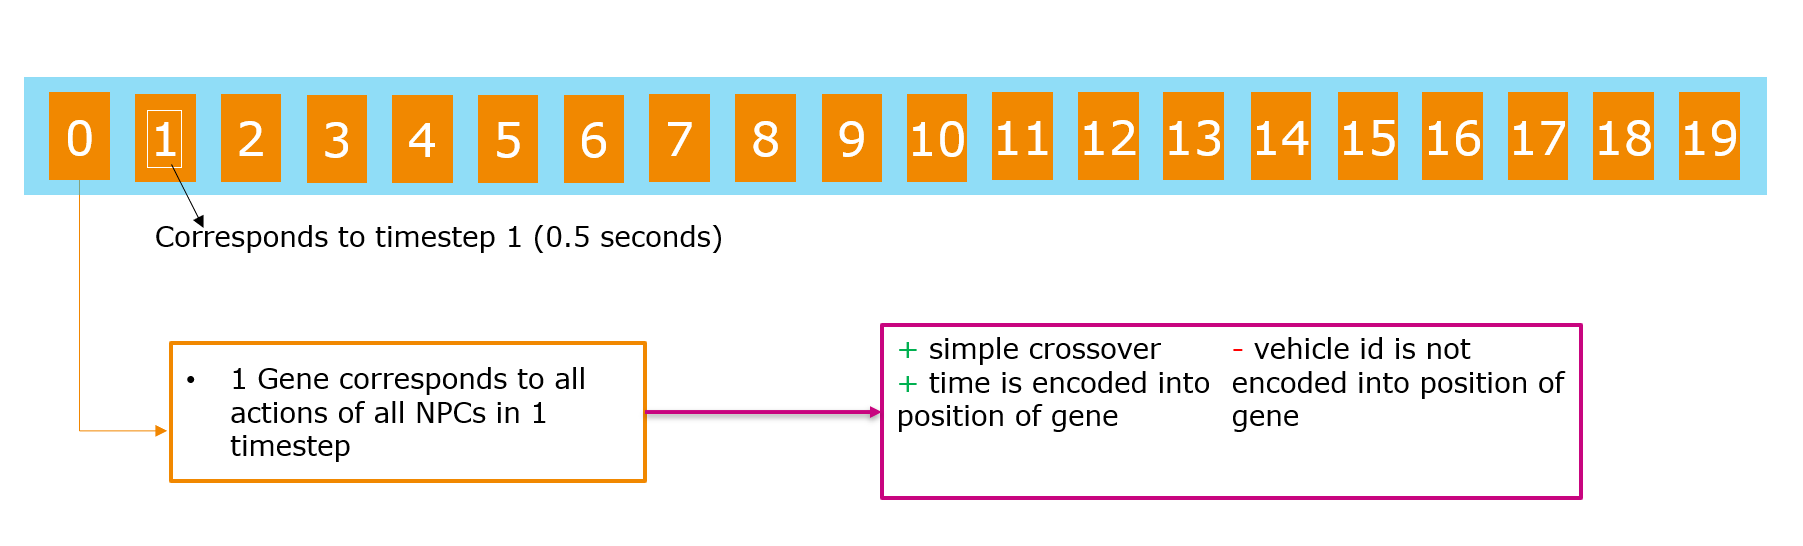
\includegraphics[width=1\linewidth]{figures/time_encoding}
	\caption{Time}
	\label{figure:encoding:chromosome:time}
\end{figure}


Given the previously stated simulation time of 35 seconds, each chromosome has a length of $35 * 2 = 70$ genes. Each gene consits of $number\_of\_actors$ actions.
Crossover can thus only move all actions of a timestep at once, modifing between actions of the same timestep can only be done using mutation. If this is desired will be seen in the next chapters.


\paragraph{TimeNPC}
The second encoding has the name "TimeNPC", and is somewhat differently structured. Now, genes only hold 1 action, encoding now not only the timestep, but also the actor id in the position of the gene inside the chromosome. Now, each actors actions will be listed one after another. This is visualized in figure \ref{figure:encoding:chromosome:time_npc}.

\begin{figure}[ht] 
	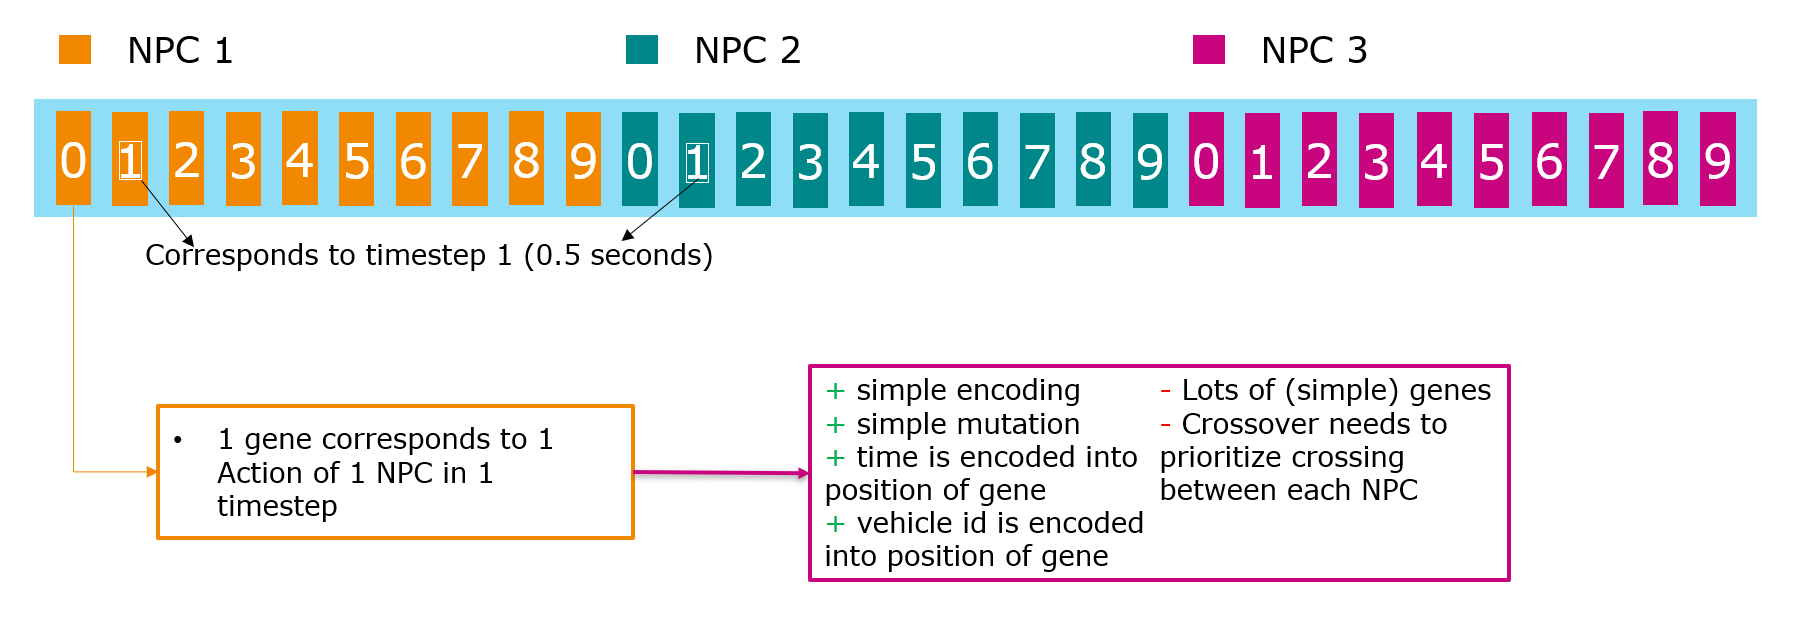
\includegraphics[width=1\linewidth]{figures/time_npc_encoding}
	\caption{Time + NPC}
	\label{figure:encoding:chromosome:time_npc}
\end{figure}

Now, each gene has a length of $1$ and each chromosome now has a length of $35 * 2 * number\_of\_actors$, which makes them much longer compared to the previous encoding. This now allows the crossover operation to modify only specific actions of one timesstep. Previously this was not possible.

However for this encoding to make sense, the crossover operations "OnePoint" and "TwoPoint" had to be modified as follows. In an example of 10 NPCs, the operations will be executed for each NPC separately. Otherwise these two operations would have only had an effect on 1 or 2 different NPCs. For the reaiming NPCs, their actions would stay the same.

\subsubsection{Gene}
Two different encodings for genes were implemented as well. A gene always consits of a list, which depending on the chromosome type either has a length of $number\_of\_actors$ (In case ChromosomeEncoding == Time) or of length 1 (in case ChromosomeEncoding == TimeNPC). The following two encodings thus show the type of object, which is in these lists.

\paragraph{Integer}
The first encoding uses integer, which are translated into actions when the simulation is started. For each action, a range of integers is assigned, the larger the range, the more likely the action is chosen by the GA. Actions that have parameters are split into different ranges, according to which paramters make sense. For example ModifyTargetVelocity is split into five different parts, with different percentages, namely 50, 70, 100, 130, 160. The range of integers assigned to these parts is different. A percentage setting of 100 for example has the largest integer range assigned.
In Appendix , the probabilty of an actions can be seen. In Appendix ... the probabitly per actions of the parameters can be viewed.

These ranges were assigned based on intuition and trial and error. The encoding is visualized in \ref{figure:encoding:gene:int}.

TODO: Due to the cliff problem, it was decided to not use binary representations for these integers. Due to the mutation choosing the integers randomly, it is not a problem that the variables are not really "continous".

\begin{figure}[ht] 
	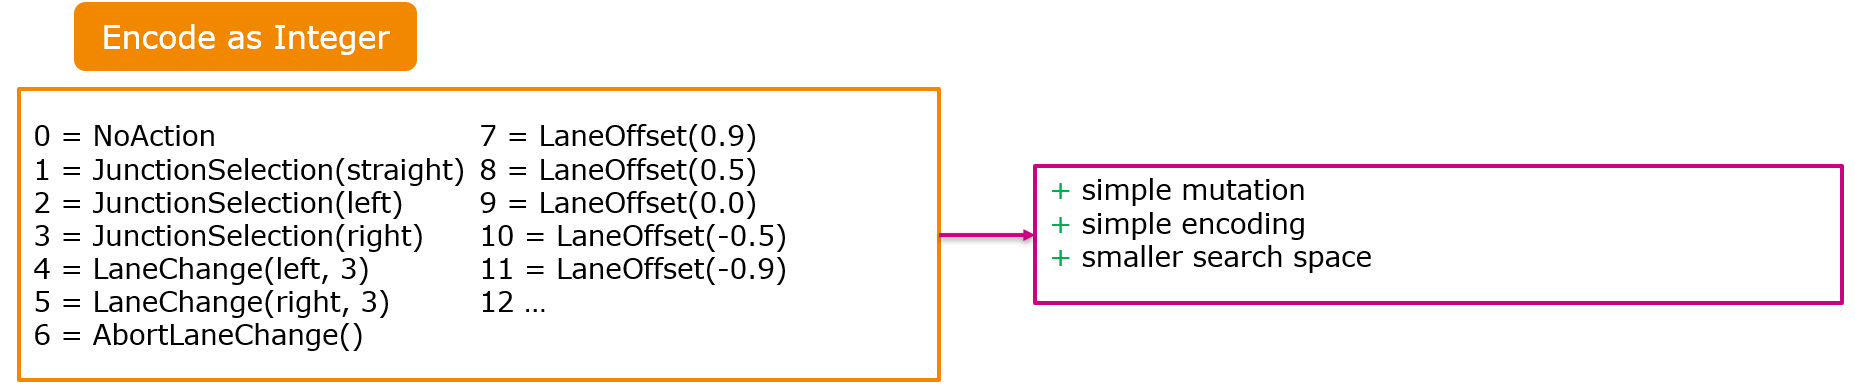
\includegraphics[width=1\linewidth]{figures/int_encoding}
	\caption{Integer}
	\label{figure:encoding:gene:int}
\end{figure}

\paragraph{Dictionary}
The second encoding is much similar to the actual actions used in the simulations. Now, no translation is necessary anymore. During generation of the individuals, each action is again selected based on different probabilities assigned to actions, which again can be viewed in Appendix ... . These probablilites are the same as for the integer encoding. However the difference is, in case an action has parameters that need to be chosen. 
For each parameter, a range and a randomness function was chosen. For example in case of the percenetage parameter in ModifyTargetVelocity, the values are selected from a GausDistribution, with mu= 100, sigma=25 and a range limit between 0 and 300.

Again, these probability functions with settings were assigned based on intuition as well as trial and error. Detailed information can be seen in Appendix...

Figure \ref{figure:encoding:gene:dict} shows a visualization.

\begin{figure}[ht] 
	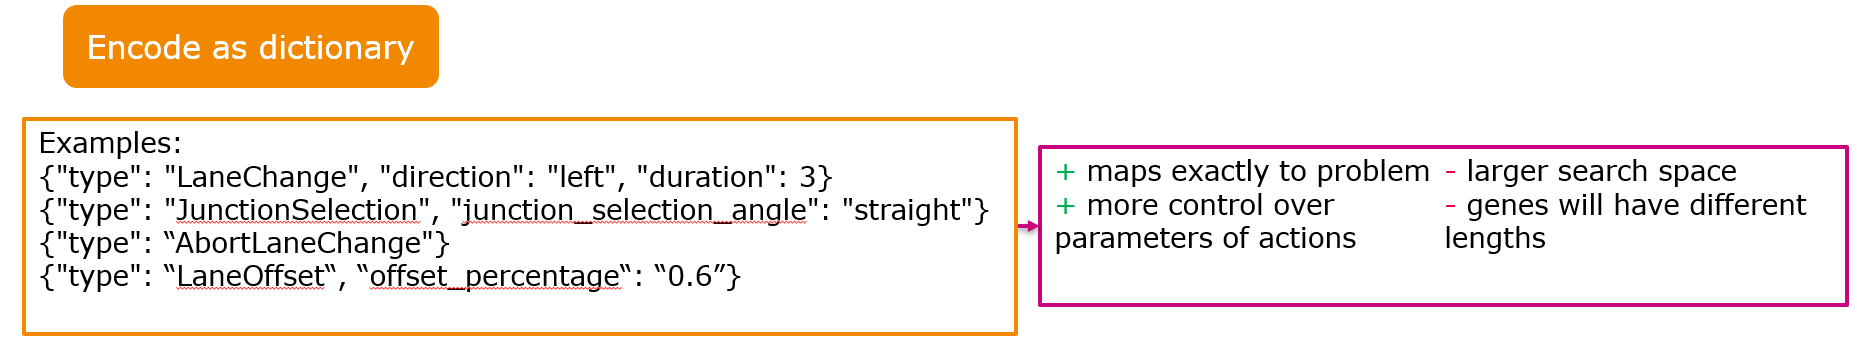
\includegraphics[width=1\linewidth]{figures/dict_encoding}
	\caption{Dictionary}
	\label{figure:encoding:gene:dict}
\end{figure}

\subsection{Cost Function}
\label{implementation:cost_function}
\todo{Suggestion florian: better explain cost values (e.g. 3500 means no emergency break...)}

Cost function is a bit difficult, as we are only using internal values. No ADAS/AD system is tested and we thus have to work with what we got.
This is the code of the cost function:

\begin{lstlisting}[language=Python, tabsize=4]
SEPS_PER_SECOND = 100
# allow emergency breaks to last only 3 seconds
MAX_DURATION = 3 * STEPS_PER_SECOND

cost = 0
duration_counter = 0
for i in range(len(result["ego_emergency_stop"])):
	if not result["ego_emergency_stop"][i]:
		# base cost in case of no current emergency break
		cost = cost + 1
		duration_counter = 0
	else:
		if duration_counter > MAX_DURATION:
			# increase cost if emergency break max duration is exceeded
			cost = cost + 10
		duration_counter += 1
return cost
\end{lstlisting}
result["ego\_emergency\_stop"] is a list with the length $100 * simulation\_duration\_seconds$ (because 100hz). It contains a boolean per step, if the EGO vehicle has initiated an emergency stop.

It would have been interesting to not only test for emergency stops (which will make the NPCs try to get the EGO to hard break often) but also improve time to collison (TTC), as was done by \todo{Ref florian}. However by the time of starting the testing, no working TTC functionality was implemented. Thus, only the emergency break cost function is used by the GA to be optimized.


\section{Behavior Tree}
A behavior tree is a decision tree. \todo{insert a good introduction to BT}
Depending on the functionality under test, it is possible to let the EGO vehicle be controlled by a Behaviour Tree. This makes sense if for example a functionilty like AEB is tested, where only the breaks are controlled. In case of a full driving stack, no Behaviour Tree would be used.

The general idea is to have an EGO vehicle moving in a "relateable" manner trough the world. It will try to dodge standing or slow moving obstacles. This needs to be done in a determinisitc manner in order to no introduce randomness into the simulation.

For this, Behaviour Tree is used. While it has access to the same Action Interface (described in section \ref{implementation:action_interface}) as the Genetic Algorithm, it is more tightly integrated with the Traffic Manger. While the Genetic Algorithm only ingests the results generated by the Simulation with the cost function, the Behaviour Tree needs access to internal functions during the simulation. The following figure shows the behaviour tree implemented.

\iffalse
\begin{figure}[H]
	\centering
	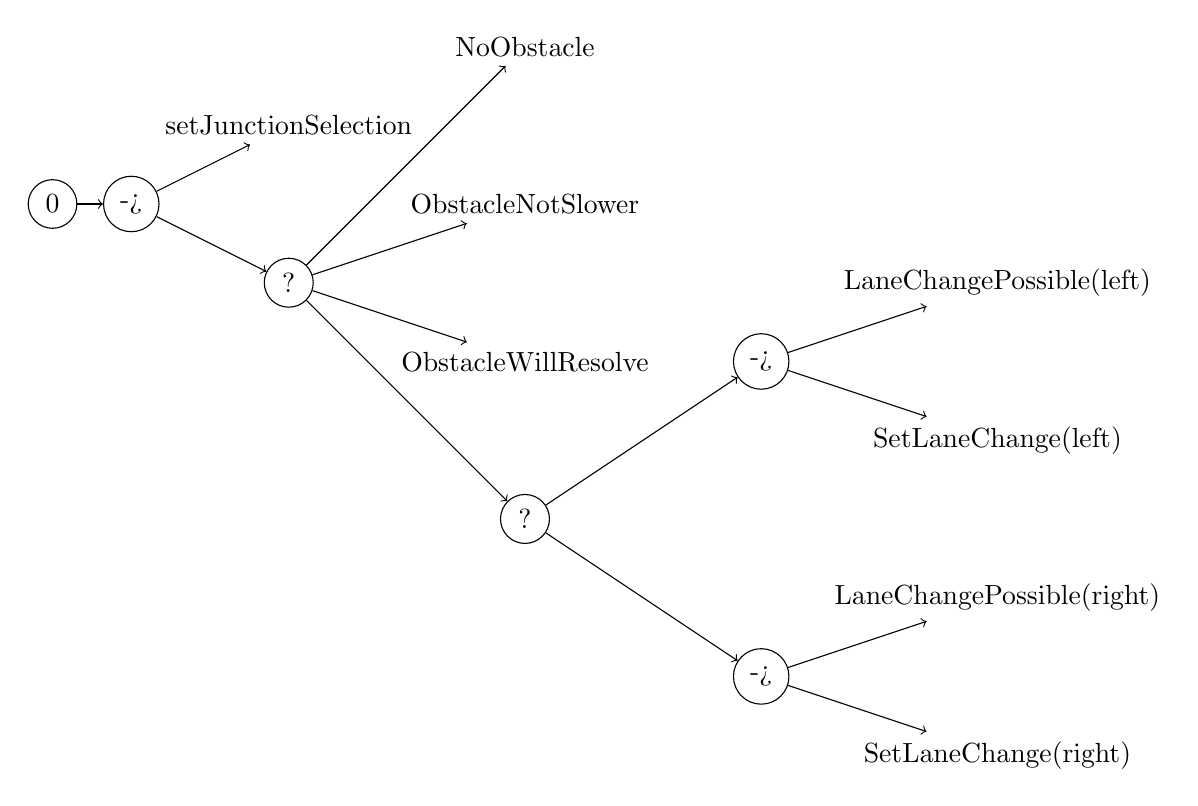
\begin{tikzpicture}
		% Define 1 2 3
		\node[draw, circle] (NodeStart) at (0,0) {0};
		\node[draw, circle] (Sequence1) at (1,0) {->};
		\draw[->] (NodeStart) -- (Sequence1);
		
		\node (Action1) at (3,1) {setJunctionSelection};
		\node[draw, circle] (OR1) at (3,-1) {?};
		\draw[->] (Sequence1) -- (Action1);
		\draw[->] (Sequence1) -- (OR1);

		\node (Action21) at (6,2) {NoObstacle};
		\node (Action22) at (6,0) {ObstacleNotSlower};
		\node (Action23) at (6,-2) {ObstacleWillResolve};
		\node[draw, circle] (OR2) at (6,-4) {?};
		\draw[->] (OR1) -- (Action21);
		\draw[->] (OR1) -- (Action22);
		\draw[->] (OR1) -- (Action23);
		\draw[->] (OR1) -- (OR2);
		
		\node[draw, circle] (Sequence31) at (9,-2) {->};
		\node[draw, circle] (Sequence32) at (9,-6) {->};
		\draw[->] (OR2) -- (Sequence31);
		\draw[->] (OR2) -- (Sequence32);
		
		\node (Action41) at (12,-1) {LaneChangePossible(left)};
		\node (Action42) at (12,-3) {SetLaneChange(left)};
		\node (Action43) at (12,-5) {LaneChangePossible(right)};
		\node (Action44) at (12,-7) {SetLaneChange(right)};
		\draw[->] (Sequence31) -- (Action41);
		\draw[->] (Sequence31) -- (Action42);
		\draw[->] (Sequence32) -- (Action43);
		\draw[->] (Sequence32) -- (Action44);
		
		
	\end{tikzpicture}
	\caption{Used Behaviour Tree}
\end{figure}
\fi

\begin{figure}[ht]
	\centering
	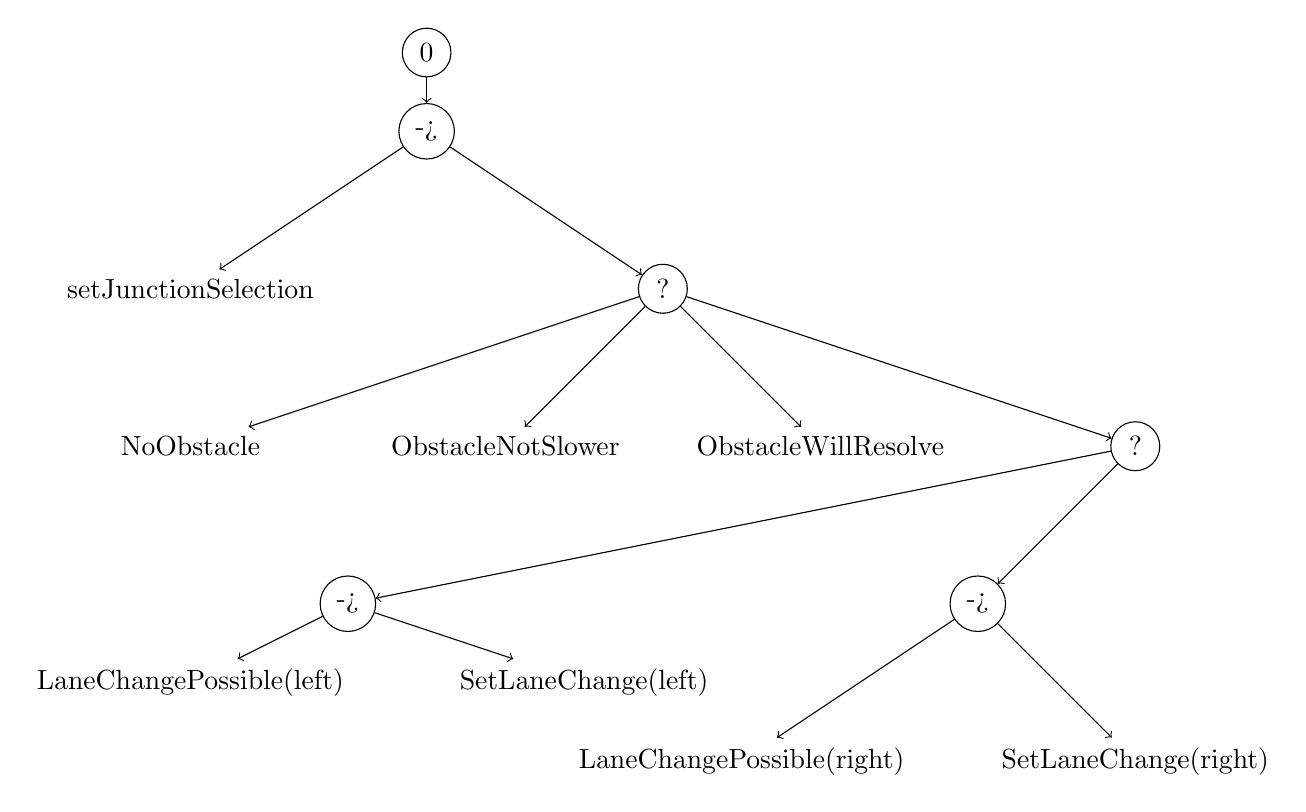
\begin{tikzpicture}
		% Define 1 2 3
		\node[draw, circle] (NodeStart) at (0,0) {0};
		\node[draw, circle] (Sequence1) at (0,-1) {->};
		\draw[->] (NodeStart) -- (Sequence1);
		
		\node (Action1) at (-3,-3) {setJunctionSelection};
		\node[draw, circle] (OR1) at (3,-3) {?};
		\draw[->] (Sequence1) -- (Action1);
		\draw[->] (Sequence1) -- (OR1);
		
		\node (Action21) at (-3,-5) {NoObstacle};
		\node (Action22) at (1,-5) {ObstacleNotSlower};
		\node (Action23) at (5,-5) {ObstacleWillResolve};
		\node[draw, circle] (OR2) at (9,-5) {?};
		\draw[->] (OR1) -- (Action21);
		\draw[->] (OR1) -- (Action22);
		\draw[->] (OR1) -- (Action23);
		\draw[->] (OR1) -- (OR2);
		
		\node[draw, circle] (Sequence31) at (-1,-7) {->};
		\node[draw, circle] (Sequence32) at (7,-7) {->};
		\draw[->] (OR2) -- (Sequence31);
		\draw[->] (OR2) -- (Sequence32);
		
		\node (Action41) at (-3,-8) {LaneChangePossible(left)};
		\node (Action42) at (2,-8) {SetLaneChange(left)};
		\node (Action43) at (4,-9) {LaneChangePossible(right)};
		\node (Action44) at (9,-9) {SetLaneChange(right)};
		\draw[->] (Sequence31) -- (Action41);
		\draw[->] (Sequence31) -- (Action42);
		\draw[->] (Sequence32) -- (Action43);
		\draw[->] (Sequence32) -- (Action44);
		
		
	\end{tikzpicture}
	\caption{Used Behaviour Tree}
\end{figure}


Starting out, \todo{Explain BT}


\chapter{Hyperparameter Tuning}
\label{chap:hyperparameter_tuning}
The performance of a genetic algorithm is significantly influenced by its control parameters. Performant settings on one particular fitness landscape might not be on appropriate a different one~\cite{kacprzyk_parameter_2007}. This chapter will focus on tuning the genetic algorithm to perform well on the given cost function. First, a choice on the optimal population size is made. Afterwards, the Taguchi method is used for tuning the remaining hyperparameter.

\section{Simulation Setup}
\label{sect:hyperparameter_tuning:simulation_setup}
Two workstations were available for running all of the following simulations. The first workstation had an Intel Core i7-9700K and a GeForce RTX 2070 SUPER with 32 GB of RAM. The second workstation had an Intel Core i7-6850K as well as two Nvidia GeForce GTX 1080, also equipped with 32 GB of RAM. On both systems, Kubuntu 20.04 LTS was the operating system.

As defined in Chapter \ref{chap:implementation}, each genetic algorithm will run for 30 generations. Additionally one simulation will have a duration of 35 seconds. On a single workstation, approximately 3 hours and 50 minutes are needed to complete one genetic algorithm with a population size of 96. This time indication, however, is influenced by the number of actors. The street map 'Town 10' from the driving simulator Carla\footnote{\href{https://carla.readthedocs.io/en/latest/map_town10/}{https://carla.readthedocs.io/en/latest/map\_town10/}} will be used for all experiments. It has an adequate size, yet is not too big, and allows for interesting manoeuvrers. To minimize the number of needed tests, a single start scenario was utilized for tuning the control parameter. It is referred to as 'start scenario 1' can be seen in the Appendix at Figure \ref{fig:appendix:start_scenarios_1_2}. In Chapter \ref{chap:evaluation}, the performance of the tuned genetic algorithm on different start scenarios will be investigated.

\section{Population}
\label{sect:hyperparameter_tuning:population}
Finding a suitable population size is of high importance to a genetic algorithm. On one hand, a population that is too small might result in less diverse runs of the genetic algorithm, on the other hand, if the population size is too high, the simulations will become too costly (see Section \ref{sect:foundations:genetic_algorithm}).

In order to evaluate the best population size, other hyperparameters first have to be fixated. Grefenstette~\cite{grefenstette_optimization_1986} suggests that a range of control parameter will already lead to acceptable performance, yet optimal performance needs tuning. De Jong~\cite{kacprzyk_parameter_2007} complements these findings, adding that the 'sweat spot' for control parameters of genetic algorithms is reasonably large and easy to find. A default set of static parameter values is generally speaking sufficient. Following this advice, the most suitable population parameters will now be evaluated by fixating the remaining hyperparameters to a small range of suggested values from the literature.

\subsection{Identifying Suggested Hyperparameter Settings from Existing Literature}
After reviewing various literature regarding control parameter of genetic algorithms, no clear consensus emerged. Mills et al.~\cite{mills_determining_2015} came to a similar conclusion, mentioning the inconsistencies between findings during their literature review and highlighting the conflicting evidence regarding \enquote{key GA control parameter}. Table \ref{tab:hyperparameter_tuning:ga_hyperparameters} aims to provide a short, though not exhaustive, overview on different control parameter settings used in the literature. This compilation does not claim to cover the entire scope of available research in this domain, rather it served as a focused effort to identify usable hyperparameters.

\begin{table}[ht]
	\centering
	\begin{tabular}{lcccc}
		\hline
		\textbf{Parameter Set} & \textbf{Pop} & \textbf{Cross} & \textbf{Mut} & \textbf{Sel} \\
		\hline
		De Jong~\cite{de_jong_analysis_1975} & 50 & 0.6 & 0.001 & ? \\
		Mills et al.~\cite{mills_determining_2015} & 200 & ? & Adaptive & SUS\\
		Grefenstette~\cite{grefenstette_optimization_1986} & 30 & 0.95 & 0.01 & ?\\
		Grefenstette~\cite{grefenstette_optimization_1986} & 80 & 0.45 & 0.01 & ?\\
		Almanee et al.~\cite{almanee_scenorita_2021} & 50 & 0.8 & 0.2 & ?\\
		Srinivas and Patnaik~\cite{srinivas_genetic_1994}  & 30-100 & 0.9 & 0.01 & ?\\
		Fazal et al.~\cite{fazal_estimating_2005} & 50 & 0.5 & ? & Tourn\\
		Dao et al.~\cite{dao_maximising_2016} & 200 & 0.7 & ? & Roul\\
		Naruka et al.~\cite{naruka_parameter_2019} & 200 & 0.4 & ? & Roul \\
		Jinghui Zhong et al.~\cite{jinghui_zhong_comparison_2005} & 50-250 & 0.1-0.9 & 0.05-0.25 & ?\\
		\hline
	\end{tabular}
	\caption{summary of literature review}
	\label{tab:hyperparameter_tuning:ga_hyperparameters}
\end{table}

A value between 30-200 is a commonly recommended as a population size. In order to reduce the needed computation time, a population size of 96 is defined as a maximum for the future evaluation. Crossover rates are mostly be in a range of 0.6-0.9. When it comes to the mutation rate, a low value is commonly advised. For example Grefenstette~\cite{grefenstette_optimization_1986} suggest poor performance using a rate over 0.05. Using a low mutation rate is also suggested by Whitley~\cite{whitley_genetic_1994} and Jinghui Zhong et al.~\cite{jinghui_zhong_comparison_2005}. On the other hand, Boyabatli~\cite{boyabatli_parameter_2004} found higher mutation rates for their application to be more suitable. Srinivas and Patnaik~\cite{srinivas_genetic_1994} differentiate between higher and lower population numbers, claiming that a smaller population needs higher mutation rates in order to maintain a sufficient diversity.

\subsection{Comparison of Population Size}
Based on the described research, population sizes of 32, 48, 64 and 96 will be compared. Crossover rates are set to 0.6 and 0.8. For mutation, 0.01 and 0.2 will be discussed. Further, tournament selection of 2 and 4 is used. Individual mutation probability will stay at 0.1. Chromosome encoding is set to Time and gene encoding is set to Integer.  Each run will be executed 5 times in order to reduce randomness and to make the results more robust. Each simulation will last for 30 generations. A list of all settings with the mean over 5 repetitions per population size can be seen in Table \ref{tab:hyperparameter_tuning:pop_settings_results}.

\begin{table}[ht]
	\centering
	\begin{tabular}{ c|c|cccc  }
		\hline
		Settings & Code & 32 & 48 & 64 & 96\\
		\hline
		C: 0.6, M: 0.01, TS: 2   	& A & 4.49 & 4.84 & 6.49 & 6.29 \\
		C: 0.6, M: 0.01, TS: 4		& B & 3.89 & 4.79 & 4.21 & 5.63 \\ 
		C: 0.6, M: 0.20, TS: 2 		& C & 4.38 & 4.90 & 4.98 & 6.69 \\
		C: 0.6, M: 0.20, TS: 4    	& D & 4.80 & 5.33 & 6.09 & 6.50 \\
		C: 0.8, M: 0.01, TS: 2   	& E & 4.37 & 6.08 & 5.29 & 5.84 \\
		C: 0.8, M: 0.01, TS: 4		& F & 4.48 & 4.51 & 4.46 & 6.03 \\
		C: 0.8, M: 0.20, TS: 2 		& G & 4.01 & 5.60 & 5.41 & 6.31 \\
		C: 0.8, M: 0.20, TS: 4    	& H & 4.42 & 4.95 & 7.06 & 6.91 \\
		\hline
	\end{tabular}
	\caption{population size results - mean over 5 repetitions}
	\label{tab:hyperparameter_tuning:pop_settings_results}
\end{table}

\begin{figure}[ht] 
	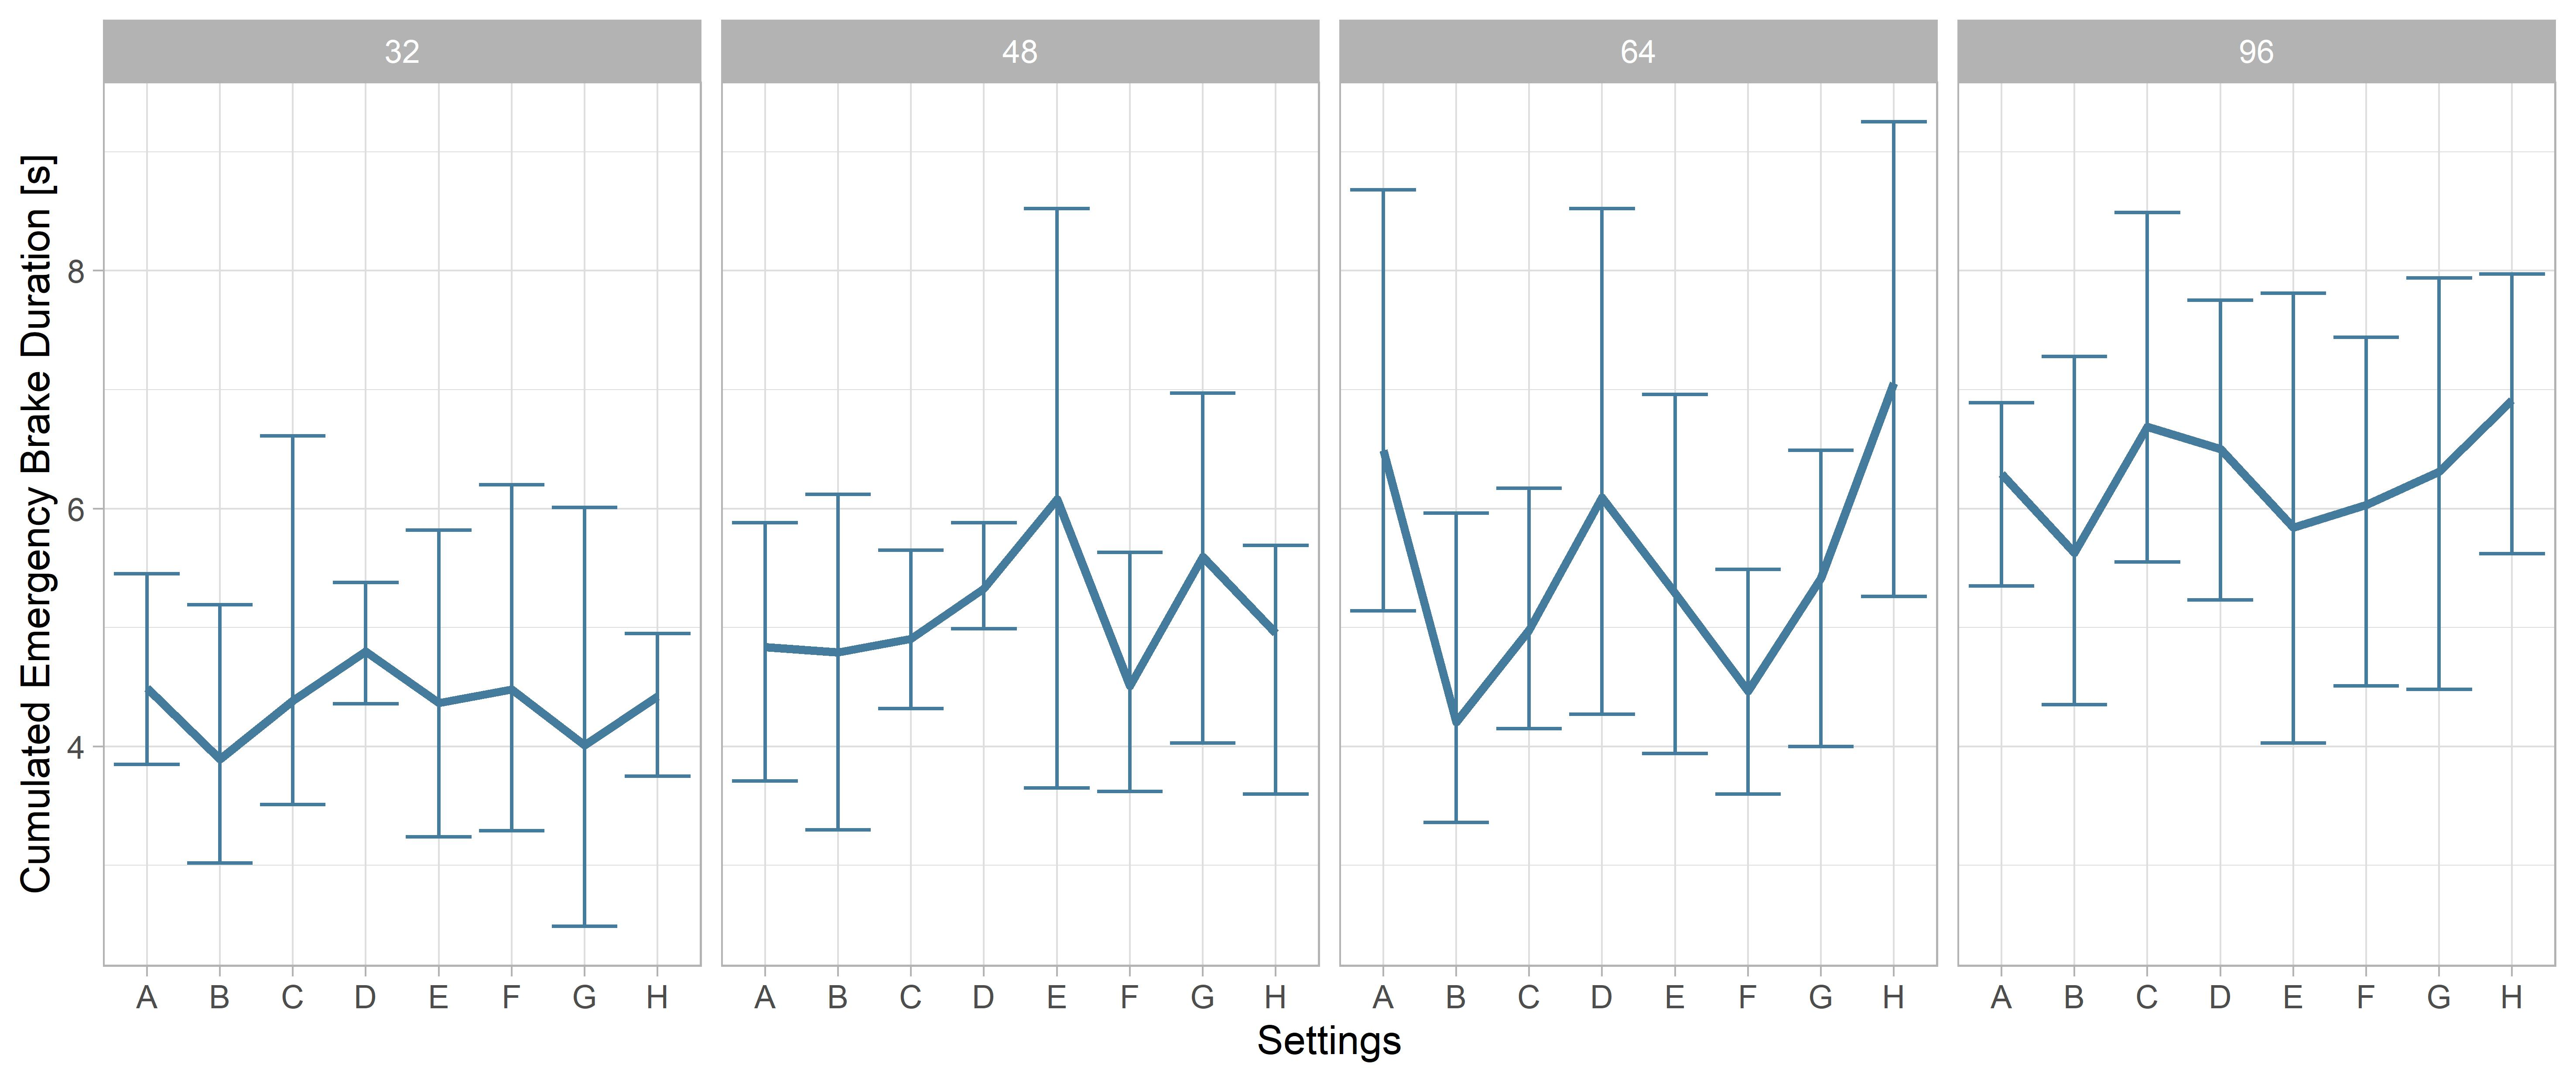
\includegraphics[width=1\linewidth]{simulations/population/plots/comparison}
	\caption{mean and error bars per population size}
	\label{fig:hyperparameter_tuning:population_results}
\end{figure}

In Figure \ref{fig:hyperparameter_tuning:population_results}, the results per population are plotted. The line corresponds to the mean, while the error bars show the spread (min to max) of all 5 repetitions. A higher spread in the results can be seen when looking at the smaller population sizes. Considering these findings, a population size of 96 was chosen. While such a high value will result in a performance impact, it was deemed more important to keep the variation low.

\section{Design of Experiment}
\label{sect:hyperparameter_tuning:design_of_experiment}
This section aims to find optimal settings for the remaining control parameters of the given problem. Following the conclusion from the previous Section \ref{sect:hyperparameter_tuning:population}, a population size of 96 will be fixated. In order to further tune the control parameter of the genetic algorithm, various different strategies can be used. Using automated approaches like 'grid search', 'bayesian optimization', 'simmulated annealing' or 'hyperband' might lead to good results with minimal effort~\cite{kacprzyk_parameter_2007}.\todo{find more references} De Jong~\cite{kacprzyk_parameter_2007} even suggests using a second, higher level genetic algorithm for the optimization process. The tuning of hyperparameter for these algorithms is however still needed. Due to performance considerations, many optimization methods did not fit the requirements. Executing one run for 30 generations takes around 3:50 hours. The high variance between runs requires a certain number of repetitions for each setting. Although two different workstations were available, the time required to execute the needed number of runs for these automated tests would exceed the available time budged. For this section, 8 repetitions were used per setting, which makes one evaluation last 30 hours.

A different approach is called design of experiment (DOE), also known as statistically designed experiments. DOE tries to find the cause and-effect relationship between the factors and the output of experiments. It uses factorial design where the variables in an experiment are named 'factors'. Each factor consists of at least two settings, with the actual number of settings being called 'levels'~\cite{yang_design_2009}. Design of experiment needs manual expertise to define which factors are possibly of importance and which settings each factor should have.

\begin{quote}
	\begin{em}
		\enquote{If the range of variable is too small, then we may miss lots of useful information. If the range is too large, then the extreme values might give infeasible experimental runs.}~\cite{yang_design_2009}
	\end{em}
\end{quote}

Subsequently, main effects and interactions can be calculated to find the best settings per factor. ANOVA (Analysis of Variance) will identify the significance of each factor and interaction. More details on these analysis tools will be provided in Section \ref{sect:hyperparameter_tuning:analysis_of_results}.

A full factorial design will test over all possible combinations of the selected factor levels. Looking at the proposed factors in Table \ref{tab:hyperparameter_tuning:settings_to_level}, 1024 runs\footnote{number of runs calculated using: \url{https://datatab.net/statistics-calculator/design-of-experiments}} are required, which is not feasible performance wise. A full factorial design has the drawback, that, as the number of factors k gets increased, the number of needed experimental runs increases exponentially, thus resulting in lengthy experiments. Yang and El-Haik~\cite{yang_design_2009} state that most of the results obtained by testing over all combinations are only used for estimating higher-order interactions, which are in most cases insignificant.

\subsection{Taguchi Method}
Various improvements to design of experiment have been but forward by Dr. Genichi Taguchi, such as reducing the influence of uncontrollable (noise) factors on processes and products as well as reducing variability~\cite{roy_primer_1990}.\todo{Ask GBT if this is true} This master's thesis will not discuss all of Taguchi's proposed considerations; for more detail Roy~\cite{roy_primer_1990} as well as Yang and El-Haik~\cite{yang_design_2009} are recommended. Taguchi's proposed design of experiment is a fractional factorial design, which requires significantly fewer runs. In fractional factorial designs, only a fraction of all possible combinations is investigated~\cite{roy_primer_1990}. While different fractional factorial designs are available, Taguchi was chosen, because he provides a simple and easy-to-follow procedure that requires only a minimal number of runs. 

\begin{quote}
	\begin{em}
		\enquote{There are many similarities between “regular” experimental design and Taguchi's experimental design. However, in a Taguchi experiment, only the main effects and two-factor interactions are considered. Higher-order interactions are assumed to be non-existent. In addition, experimenters are asked to identify which interactions might be significant before conducting the experiment, through their knowledge of the subject matter.}~\cite{yang_design_2009}
	\end{em}
\end{quote}

Taguchi predefined a number of different orthogonal arrays where each row contains the specific levels (i.e the settings) of one experiment, while the columns correspond to the factors. The researcher has the responsibility to select an array based on the individual needs~\cite{li_taguchi_2021}. Using these orthogonal arrays instead of full factorial experiments will lead to a much smaller amount of simulation runs, while the full factorial experiments \enquote{might not provide appreciably more useful information}~\cite{roy_primer_1990}.

A big drawback of using Taguchi orthogonal arrays is the inability of evaluating higher-order interaction effects. Not only are these interaction effects impossible to evaluate, but they also have a negative influence on the performance. Orthogonal array experiments perform best in cases of minimal interaction between factors. While there is still a good chance of identifying the optimum condition, especially the performance estimate can be significantly off~\cite{roy_primer_1990}. Although Yang and El-Haik~\cite{yang_design_2009} state that in many cases higher-order interaction effects in factorial designs are seldom significant, this might not be the case for genetic algorithms. For example, according to \cite{kacprzyk_parameter_2007}, control parameters of a genetic algorithm \enquote{interact in highly non-linear ways.} If the proposed method is able to provide a suitable set of hyperparameter settings will be evaluated in Chapter \ref{chap:evaluation}.

\paragraph{Selection of an Orthogonal Array}
When choosing a suitable Taguchi orthogonal array, various factors have to be taken into account. According to Yang and El-Haik~\cite{yang_design_2009}, a three step procedure needs to be followed:

\begin{enumerate}
	\item Calculate the total degree of freedom (DOF). 
	\item Based on the following two rules, a standard orthogonal array should be selected:
	\begin{enumerate}
		\item The total DOF need to be smaller than the number of runs provided by the orthogonal array.
		\item All required factor level combinations need to be accommodated by the orthogonal array.
	\end{enumerate}
	
	\item Factors have to be assigned using these rules: 
	\begin{enumerate}
		\item In case the factor level does not fit into the orthogonal array, methods such as column merging and dummy levels can be used to modify the original array.
		\item Using the linear graph and interaction table, interactions can be defined. 
		\item In case some columns are not assigned, its possible to keep these columns empty.
	\end{enumerate}
\end{enumerate}

For this design of experiment, seven factors (three 4-level factors and four 2-level factors) have been selected. The choice of factors and levels to choose was made based on experience gained on Section \ref{sect:hyperparameter_tuning:population}. In Table \ref{tab:hyperparameter_tuning:settings_to_level}, every factor with the corresponding levels is listed.

\begin{table}[ht]
	\centering
	\small
	\begin{tabular}{ l|c|cccc }
		\hline
		Factors & Code & Level 1 & Level 2 & Level 3 & Level 4\\
		\hline
		CrossoverType 		& A & one point & two point & uni$^*$ 0.1 & uni$^*$ 0.5\\
		CrossoverRate    	& B & 0.2 & 0.5 & 0.8 & 0.9\\
		MutationRate   		& C & 0.01 & 0.1 & 0.3 & 0.5\\
		ChromosomeType   	& D & Time & Time+NPC & - & -\\
		GeneType			& E & Int & Dict & - & -\\
		TournamentSize 		& F & 2 & 4 & - & -\\
		IndMutationRate		& G & 0.1 & 0.5 & - & -\\
		\hline
	\end{tabular}
\caption{control parameters (factors) with corresponding settings (levels) - ($^*$uniform)}
\label{tab:hyperparameter_tuning:settings_to_level}
\end{table}

As already stated, Taguchi allows to only test for predetermined two-factor interactions; evaluating higher-order factor interactions is not possible~\cite{yang_design_2009}. Analysing interactions comes at the cost of degrees of freedom. An interaction between ChromosomeType and GeneType might be of interest and will thus be chosen. In order to minimized the required degrees of freedom (and correspondingly the required number of experiment runs), no additional interactions will be analysed.

\subsection{Selection of a Suitable Standard Orthogonal Array}
\label{sect:hyperparameter_tuning:selection_orthogonal_array}
The total degree of freedom can be calculated using the rules provided by Yang and El-Haik~\cite{yang_design_2009}:

\begin{enumerate}
	\item 1 DOF is always used for the overall mean. 
	\item Each factor has a DOF of NumberOfLevels - 1.
	\item Two-factor interactions require a DOF of: $(n_{factor1} - 1)(n_{factor2} - 1)$ where $n$ = number of levels.
\end{enumerate}

This leads to the following calculation for the needed three 4-level factors and four 2-level factors as well as the interaction ChromosomeType-GeneType:

\begin{equation}
	\begin{split}
		DOF & = 1 + 3 * (4 - 1) + 4 * (2 - 1) + 1 * (2 - 1) * (2 - 1) \\
		& = 15
	\end{split}
	 \label{equ:hyperparam_tuning:DOF}
\end{equation}

A $L_{16}$ array seems suitable to accommodate the required 15 DOF, which can be seen in table \ref{tab:hyperparameter_tuning:L16_orhtogonal_array}.

\begin{table}[ht]
	\centering
	\begin{tabular}{ |c||c|c|c|c|c|c|c|c|c|c|c|c|c|c|c|  }
		\hline
		   & \multicolumn{15}{c|}{ $L_{16}(2^{15})$ } \\
		NO.& 1 & 2 & 3 & 4 & 5 & 6 & 7 & 8 & 9 & 10& 11& 12& 13& 14&15\\
		\hline
		1  & 1 & 1 & 1 & 1 & 1 & 1 & 1 & 1 & 1 & 1 & 1 & 1 & 1 & 1 & 1\\
		2  & 1 & 1 & 1 & 1 & 1 & 1 & 1 & 2 & 2 & 2 & 2 & 2 & 2 & 2 & 2\\
		3  & 1 & 1 & 1 & 2 & 2 & 2 & 2 & 1 & 1 & 1 & 1 & 2 & 2 & 2 & 2\\
		4  & 1 & 1 & 1 & 2 & 2 & 2 & 2 & 2 & 2 & 2 & 2 & 1 & 1 & 1 & 1\\
		5  & 1 & 2 & 1 & 1 & 1 & 2 & 2 & 1 & 1 & 2 & 2 & 1 & 1 & 2 & 2\\
		6  & 1 & 2 & 2 & 1 & 1 & 2 & 2 & 2 & 2 & 1 & 1 & 2 & 2 & 1 & 1\\
		7  & 1 & 2 & 2 & 2 & 2 & 1 & 1 & 1 & 1 & 2 & 2 & 2 & 2 & 1 & 1\\
		8  & 1 & 2 & 2 & 2 & 2 & 1 & 1 & 2 & 2 & 1 & 1 & 1 & 1 & 2 & 2\\
		9  & 2 & 1 & 2 & 1 & 2 & 1 & 2 & 1 & 2 & 1 & 2 & 1 & 2 & 1 & 2\\
		10 & 2 & 1 & 2 & 1 & 2 & 1 & 2 & 2 & 1 & 2 & 1 & 2 & 1 & 2 & 1\\
		11 & 2 & 1 & 2 & 2 & 1 & 2 & 1 & 1 & 2 & 1 & 2 & 2 & 1 & 2 & 1\\
		12 & 2 & 1 & 2 & 2 & 1 & 2 & 1 & 2 & 1 & 2 & 1 & 1 & 2 & 1 & 2\\
		13 & 2 & 2 & 1 & 1 & 2 & 2 & 1 & 1 & 2 & 2 & 1 & 1 & 2 & 2 & 1\\
		14 & 2 & 2 & 1 & 1 & 2 & 2 & 1 & 2 & 1 & 1 & 2 & 2 & 1 & 1 & 2\\
		15 & 2 & 2 & 1 & 2 & 1 & 1 & 2 & 1 & 2 & 2 & 1 & 2 & 1 & 1 & 2\\
		16 & 2 & 2 & 1 & 2 & 1 & 1 & 2 & 2 & 1 & 1 & 2 & 1 & 2 & 2 & 1\\
		\hline
	\end{tabular}
	\caption{ $L_{16}(2^{15})$ taguchi orthogonal array taken from Roy~\cite{roy_primer_1990}}
	\label{tab:hyperparameter_tuning:L16_orhtogonal_array}
\end{table}

The 4-level factors need additional space, which will be generated using column merging, while the interaction will need to be assigned as well.
Either an interaction table or linear graphs of the $L_{16}$ array can be used for both column merging and interaction assignment~\cite{danacioglu_taguchi_2005}. Both illustrate the interaction relationships in the orthogonal array~\cite{yang_design_2009}.
The linear graph is more straight forward and will be the selected approach. While there are multiple linear graphs for the $L_{16}$ array, Figure \ref{fig:hyperparameter_tuning:linear_graph} describes the graph which best fits the requirements from Table \ref{tab:hyperparameter_tuning:settings_to_level}. If no suitable graph is found, they can be modified using rules described by Danacıoğlu and Muluk~\cite{danacioglu_taguchi_2005}.

\begin{figure}[H]
	\centering
	\begin{tikzpicture}
		% Define 1 2 3
		\node (Node2) at (0,0) {2};
		\node (Middle12) at (0,1) {};
		\node (Eclipse12) at (-0.8,0) {};
		\node (Node1) at (0,2) {1};
		
		\draw (Node2) -- node[midway, right] {3} (Node1);
		
		
		% Define 4 8 12
		\node (Node8) at (2,0) {8};
		\node (Middle84) at (2,1) {};
		\node (Eclipse84) at (1.2,0) {};
		\node (Node4) at (2,2) {4};
		
		\draw (Node8) -- node[midway, right] {12} (Node4);
		
		% Define 5 15 10
		\node (Node10) at (4,0) {10};
		\node (Middle105) at (4,1) {};
		\node (Eclipse105) at (3.2,0) {};
		\node (Node5) at (4,2) {5};
		
		\draw (Node10) -- node[midway, right] {15} (Node5);
		
		% Define 7 9 14
		\node (Node9) at (6,0) {9};
		\node (Node7) at (6,2) {7};
		
		\draw (Node9) -- node[midway, right] {14} (Node7);
		
		% Define 6 11 13
		\node (Node11) at (8,0) {11};
		\node (Node6) at (8,2) {6};
		
		\draw (Node11) -- node[midway, right] {13} (Node6);
	\end{tikzpicture}
	\caption{linear graph of $L_{16}(2^{15})$ taken from Yang and El-Haik~\cite{yang_design_2009}}
	\label{fig:hyperparameter_tuning:linear_graph}
\end{figure}

In a Taguchi linear graph, both nodes and connections represent columns in the orthogonal array. The interaction between two nodes is described by the connecting line~\cite{taguchi_taguchis_2005}. This is useful for both analysing interactions between columns as well as combining (merging) interacting columns in case a higher factor is needed.

\paragraph{Column Merging}
A, B and C are 4-level factors. The currently selected orthogonal array only fits 2-level factors. Through column merging, it is possible to extend columns to accommodate higher-order levels. As calculated in Equation \ref{equ:hyperparam_tuning:DOF}, a 4-level column requires three degrees of freedom, thus three 2-level columns need to be merged. Column merging needs the to-be-merged columns to be part of an interaction group~\cite{yang_design_2009}. The available interaction groups are visualized by the linear graph in Figure \ref{fig:hyperparameter_tuning:linear_graph}. Three 2-level interaction columns need to be selected first. One column is discarded and the remain two columns are merged using the rules in Table \ref{tab:hyperparameter_tuning:merging_rules}.

\begin{table}[ht]
	\centering
	\begin{tabular}{ |ccccccc|  }
		\hline
		\multicolumn{3}{|c}{ OLD COLUMN } & & & & NEW COLUMN \\
		\hline
		& 1 & 1 & & -> & & 1\\
		& 1 & 2 & & -> & & 2\\
		& 2 & 1 & & -> & & 3\\
		& 2 & 2 & & -> & & 4\\
		\hline
	\end{tabular}
	\caption{merging rules taken from Roy~\cite{roy_primer_1990}}
	\label{tab:hyperparameter_tuning:merging_rules}
\end{table}

The 4-level factor can then be assigned to this newly generated column. Because three 4-level factors are needed for the current experiment, a total of nine 2-level columns have to be merged.

\paragraph{Assigning Interactions}
The interaction between both 2-level factors is also assigned by utilizing the linear graph. An interaction between ChromosomeType and GeneType seems possible, thus D and E will be assigned to connected nodes in the linear graph. The resulting graph can be seen in Figure \ref{fig:hyperparameter_tuning:linear_graph_assigned}. An interaction between F and G can not be investigated, as the chosen orthogonal array is not able to fit the additional 1 degree of freedom (see Equation \ref{equ:hyperparam_tuning:DOF}).

\begin{figure}[H]
	\centering
	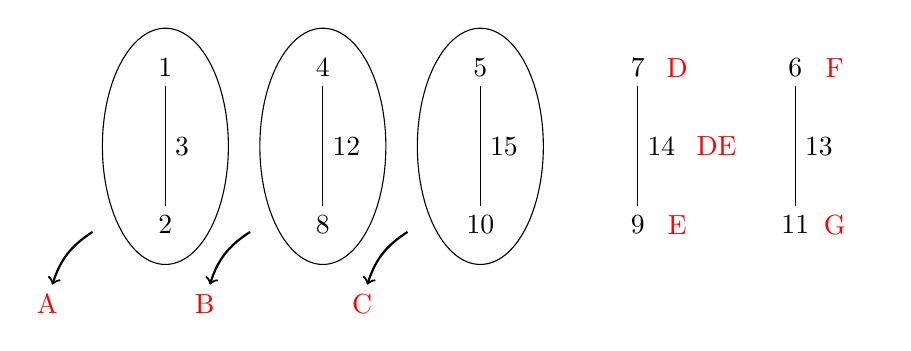
\begin{tikzpicture}
		% Define 1 2 3
		\node (Node2) at (0,0) {2};
		\node (Middle12) at (0,1) {};
		\node (Eclipse12) at (-0.8,0) {};
		\node (Node1) at (0,2) {1};
		\node[red] (A) at (-1.5, -1) {A};
	
		\draw (Node2) -- node[midway, right] {3} (Node1);
		\draw (Middle12) ellipse (0.8cm and 1.5cm);
		\draw[->, thick] (Eclipse12) to[bend right=20] (A);
		
		
		% Define 4 8 12
		\node (Node8) at (2,0) {8};
		\node (Middle84) at (2,1) {};
		\node (Eclipse84) at (1.2,0) {};
		\node (Node4) at (2,2) {4};
		\node[red] (B) at (0.5, -1) {B};
		
		\draw (Node8) -- node[midway, right] {12} (Node4);
		\draw (Middle84) ellipse (0.8cm and 1.5cm);
		\draw[->, thick] (Eclipse84) to[bend right=20] (B);
		
		% Define 5 15 10
		\node (Node10) at (4,0) {10};
		\node (Middle105) at (4,1) {};
		\node (Eclipse105) at (3.2,0) {};
		\node (Node5) at (4,2) {5};
		\node[red] (C) at (2.5, -1) {C};
		
		\draw (Node10) -- node[midway, right] {15} (Node5);
		\draw (Middle105) ellipse (0.8cm and 1.5cm);
		\draw[->, thick] (Eclipse105) to[bend right=20] (C);
		
		% Define 7 9 14
		\node (Node9) at (6,0) {9};
		\node (Node7) at (6,2) {7};
		\node[red] (E) at (6.5,0) {E};
		\node[red] (D) at (6.5,2) {D};
		\node[red] (DE) at (7,1) {DE};
		
		\draw (Node9) -- node[midway, right] {14} (Node7);
		
		
		% Define 6 11 13
		\node (Node11) at (8,0) {11};
		\node (Node6) at (8,2) {6};
		\node[red] (G) at (8.5,0) {G};
		\node[red] (F) at (8.5,2) {F};
		\node (FG) at (9,1) {};
		
		\draw (Node11) -- node[midway, right] {13} (Node6);
	\end{tikzpicture}
\caption{modified linear graph}
\label{fig:hyperparameter_tuning:linear_graph_assigned}
\end{figure}

Combining columns 1 2 3 to A, 4 8 12 to B and 5 10 15 to C using rules defined by Table \ref{tab:hyperparameter_tuning:merging_rules} is done in Table \ref{tab:hyperparameter_tuning:merging_columns}. Removing the old and inserting the new columns in the table and transcoding 7 to D, 9 to E, 14 to DE, 6 to F and 11 to G results in the final Table \ref{tab:hyperparameter_tuning:final_taguchi}.

\begin{table}[ht]
	\centering
	\begin{tabular}{ |c||cccc|cccc|cccc|  }
		\hline
		NO.& 1 & 2 & & \sout{3} & 4 & 8 & &  \sout{12} & 5 & 10 & &  \sout{15}\\
		\hline
		1  & \multicolumn{4}{c}{\sout{1 1} > 1 } & \multicolumn{4}{|c|}{\sout{1 1} > 1 } & \multicolumn{4}{c|}{\sout{1 1} > 1 }\\
		2  & \multicolumn{4}{c}{\sout{1 1} > 1 } & \multicolumn{4}{|c|}{\sout{1 2} > 2 } & \multicolumn{4}{c|}{\sout{1 2} > 2 }\\
		3  & \multicolumn{4}{c}{\sout{1 1} > 1 } & \multicolumn{4}{|c|}{\sout{2 1} > 3 } & \multicolumn{4}{c|}{\sout{2 1} > 3 }\\
		4  & \multicolumn{4}{c}{\sout{1 1} > 1 } & \multicolumn{4}{|c|}{\sout{2 2} > 4 } & \multicolumn{4}{c|}{\sout{2 2} > 4 }\\
		5  & \multicolumn{4}{c}{\sout{1 2} > 2 } & \multicolumn{4}{|c|}{\sout{1 1} > 1 } & \multicolumn{4}{c|}{\sout{1 2} > 2 }\\
		6  & \multicolumn{4}{c}{\sout{1 2} > 2 } & \multicolumn{4}{|c|}{\sout{1 2} > 2 } & \multicolumn{4}{c|}{\sout{1 1} > 1 }\\
		7  & \multicolumn{4}{c}{\sout{1 2} > 2 } & \multicolumn{4}{|c|}{\sout{2 1} > 3 } & \multicolumn{4}{c|}{\sout{2 2} > 4 }\\
		8  & \multicolumn{4}{c}{\sout{1 2} > 2 } & \multicolumn{4}{|c|}{\sout{2 2} > 4 } & \multicolumn{4}{c|}{\sout{2 1} > 3 }\\
		9  & \multicolumn{4}{c}{\sout{2 1} > 3 } & \multicolumn{4}{|c|}{\sout{1 1} > 1 } & \multicolumn{4}{c|}{\sout{2 1} > 3 }\\
		10 & \multicolumn{4}{c}{\sout{2 1} > 3 } & \multicolumn{4}{|c|}{\sout{1 2} > 2 } & \multicolumn{4}{c|}{\sout{2 2} > 4 }\\
		11 & \multicolumn{4}{c}{\sout{2 1} > 3 } & \multicolumn{4}{|c|}{\sout{2 1} > 3 } & \multicolumn{4}{c|}{\sout{1 1} > 1 }\\
		12 & \multicolumn{4}{c}{\sout{2 2} > 3 } & \multicolumn{4}{|c|}{\sout{2 2} > 4 } & \multicolumn{4}{c|}{\sout{1 2} > 2 }\\
		13 & \multicolumn{4}{c}{\sout{2 2} > 4 } & \multicolumn{4}{|c|}{\sout{1 1} > 1 } & \multicolumn{4}{c|}{\sout{2 2} > 4 }\\
		14 & \multicolumn{4}{c}{\sout{2 2} > 4 } & \multicolumn{4}{|c|}{\sout{1 2} > 2 } & \multicolumn{4}{c|}{\sout{2 1} > 3 }\\
		15 & \multicolumn{4}{c}{\sout{2 2} > 4 } & \multicolumn{4}{|c|}{\sout{2 1} > 3 } & \multicolumn{4}{c|}{\sout{1 2} > 2 }\\
		16 & \multicolumn{4}{c}{\sout{2 2} > 4 } & \multicolumn{4}{|c|}{\sout{2 2} > 4 } & \multicolumn{4}{c|}{\sout{1 1} > 1 }\\
		\hline
	\end{tabular}
	\caption{Building 4 Level columns from 2 Level columns}
	\label{tab:hyperparameter_tuning:merging_columns}
\end{table}

\begin{table}[ht]
	\centering
	\begin{tabular}{ |c||c|c|c|c|c|c|c|c|  }
		\hline
		NO.& A & B & C & D & E & F & G & DE\\
		\hline
		1  & 1 & 1 & 1 & 1 & 1 & 1 & 1 & 1\\
		2  & 1 & 2 & 2 & 1 & 2 & 1 & 2 & 2\\
		3  & 1 & 3 & 3 & 2 & 1 & 2 & 1 & 2\\
		4  & 1 & 4 & 4 & 2 & 2 & 2 & 2 & 1\\
		5  & 2 & 1 & 2 & 2 & 1 & 2 & 2 & 2\\
		6  & 2 & 2 & 1 & 2 & 2 & 2 & 1 & 1\\
		7  & 2 & 3 & 4 & 1 & 1 & 1 & 2 & 1\\
		8  & 2 & 4 & 3 & 1 & 2 & 1 & 1 & 2\\
		9  & 3 & 1 & 3 & 2 & 2 & 1 & 2 & 1\\
		10 & 3 & 2 & 4 & 2 & 1 & 1 & 1 & 2\\
		11 & 3 & 3 & 1 & 1 & 2 & 2 & 2 & 2\\
		12 & 3 & 4 & 2 & 1 & 1 & 2 & 1 & 1\\
		13 & 4 & 1 & 4 & 1 & 2 & 2 & 1 & 2\\
		14 & 4 & 2 & 3 & 1 & 1 & 2 & 2 & 1\\
		15 & 4 & 3 & 2 & 2 & 2 & 1 & 1 & 1\\
		16 & 4 & 4 & 1 & 2 & 1 & 1 & 2 & 2\\
		\hline
	\end{tabular}
	\caption{final version of orthogonal array}
	\label{tab:hyperparameter_tuning:final_taguchi}
\end{table}


\subsection{Result Analysis}
\label{sect:hyperparameter_tuning:analysis_of_results}
Table \ref{tab:hyperparameter_tuning:final_taguchi} will provide the settings for all needed test runs (the interaction column DE can be ignored until the evaluation). Transcoding all factors and levels to get the corresponding setting is done in Table \ref{tab:hyperparameter_tuning:settings_to_level}. Every setting will be repeated 8 times to reduce randomness and gain information about variance. Running the genetic algorithm with these 16 different settings each repeated 8 times took 10 days on the two workstations described in Section \ref{sect:hyperparameter_tuning:simulation_setup}. The results are found in the Appendix at Table \ref{tab:appendix:hyperparameter_tuning_final_taguchi}.

\subsubsection{ANOVA}
ANOVA analysis (analysis of variance) will provide information on the magnitude of contribution of the main effects and interactions. The calculation of ANOVA on a Taguchi experiment is the same as for a classical design of experiment~\cite{yang_design_2009}. Calculating ANOVA was done with the programming language R\footnote{\href{https://www.r-project.org/}{https://www.r-project.org/}} and the result can be seen in Table \ref{tab:taguchi:anova_results}.

\begin{table}[ht]
	\centering
	\begin{tabular}{lrrrrr}
		\hline
		& Df & Sum Sq & Mean Sq & F value & Pr($>$F) \\ 
		\hline
		A & 3 & 23.89 & 7.96 & 6.59 & 0.0004 \\ 
		B & 3 & 5.00 & 1.67 & 1.38 & 0.2532 \\ 
		C & 3 & 34.32 & 11.44 & 9.46 & 0.0000 \\ 
		D & 1 & 3.88 & 3.88 & 3.21 & 0.0759 \\ 
		E & 1 & 0.35 & 0.35 & 0.29 & 0.5912 \\ 
		F & 1 & 18.91 & 18.91 & 15.64 & 0.0001 \\ 
		G & 1 & 6.98 & 6.98 & 5.77 & 0.0179 \\ 
		D:E & 1 & 4.10 & 4.10 & 3.40 & 0.0680 \\ 
		Residuals & 113 & 136.60 & 1.21 &  &  \\ 
		\hline
	\end{tabular}
	\caption{ANOVA results}
	\label{tab:taguchi:anova_results}
\end{table}

The sum of squares column tells how much of the total variation is explained by the model. The variance is broken down into the factors A-G along with the interaction D:E. The residual sum of squares shows the difference between the model's prediction versus what was actually observed (i.e the variance that can not be explained by the model)~\cite{field_discovering_2012}. The F ratio (or value) measures the ratio of variance explained by the factor and the variation explained by the error term~\cite{field_discovering_2012}. Simply speaking, how good is the model versus how bad is the model. Finally, the p-value (in column labelled Pr(>F)) shows how likely the size of the given F ratio is obtained in case there is no effect on the results. Commonly, if p is smaller than 0.05, the effect can be viewed as statistically significant~\cite{field_discovering_2012}. The number of DOF is a result from the number of repetitions and can be calculated with the Equation \ref{equ:hyperparam_tuning:full_DOF} (taken from Roy~\cite{roy_primer_1990}).

\begin{equation}
	\begin{split}
		DOF & = totalNumberOfResults - 1 \\
		& = numberOfTrials * numberOfRepetitions - 1 \\
		& = 16 * 8 - 1 = 127
	\end{split}
	\label{equ:hyperparam_tuning:full_DOF}
\end{equation}

The multiple R-squared value of the model is 0.416 while the adjusted R-squared value is 0.344. Multiple R-squared gives a measure on how much variability in the outcome is explained by the predictors~\cite{field_discovering_2012}. Having only 41.6\% does not seem optimal. Field et al.~\cite{field_discovering_2012} state further that a model which generalizes well has an adjusted R-squared value that is similar to multiple R-squared, which is also not the case. The high error might possibly be explained by the huge search space in the scenario. Increasing the population and number of generations can lead to improvements, however at the cost of computational time. Whether the model, having this much of an error, will perform well compared to either a genetic algorithm build from values from the literature or compared to random search will be evaluated in Section \ref{chap:evaluation}.

\todo{Factors or Main Effects?}
Looking at the factors as well as the interaction, significant main effects can be seen. The highest F value has the main effect F (TournamentSize). The effect is significant with F(1, 112) = 15.64, p < 0.001. Next, the effect C (MutationRate) is significant with F(3, 112) = 9.46, p < 0.001. A (CrossoverType) is also significant F(3, 112) = 6.59, p < 0.001. Finally G (IndependendMutationRate) is significant with F(1, 112) = 5.77, p < 0.05.
D (ChromosomeType) and the interaction D:E will be mentioned as well with F(1, 112) = 3.21, p < 0.1 and F(1, 112) = 3.4, p < 0.1 respectively. There is not enough evidence to suggest significant main effects for the factors B (CrossoverRate) and E (GeneType). Particularly noteworthy is that the CrossoverRate does not show significant effects, which is not supported by the literature \todo{find references}. The low influence of GeneType, however, might be explained by the fact, that it does not have an impact on the action selected apart from more granularity of the parameters when Dictionary encoding is used. To calculate the percentage contribution of each factor, Equations \ref{equ:hyperparam_tuning:ss_t} and \ref{equ:hyperparam_tuning:contribution} (gathered from from Yang and El-Haik~\cite{yang_design_2009}) are used.

\begin{equation}
	\begin{split}
		SS_T & = SS_A + SS_B + SS_C + ... + SS_{error}
	\end{split}
	 \label{equ:hyperparam_tuning:ss_t}
\end{equation}

\begin{equation}
	\begin{split}
		contribution_A = SS_A / SS_T * 100
	\end{split}
	 \label{equ:hyperparam_tuning:contribution}
\end{equation}

The percentage contribution of all factors is plotted in \ref{fig:hyperparam_tuning:percentage_contribution} and again shows the high error of the model. 

\begin{figure}[ht] 
	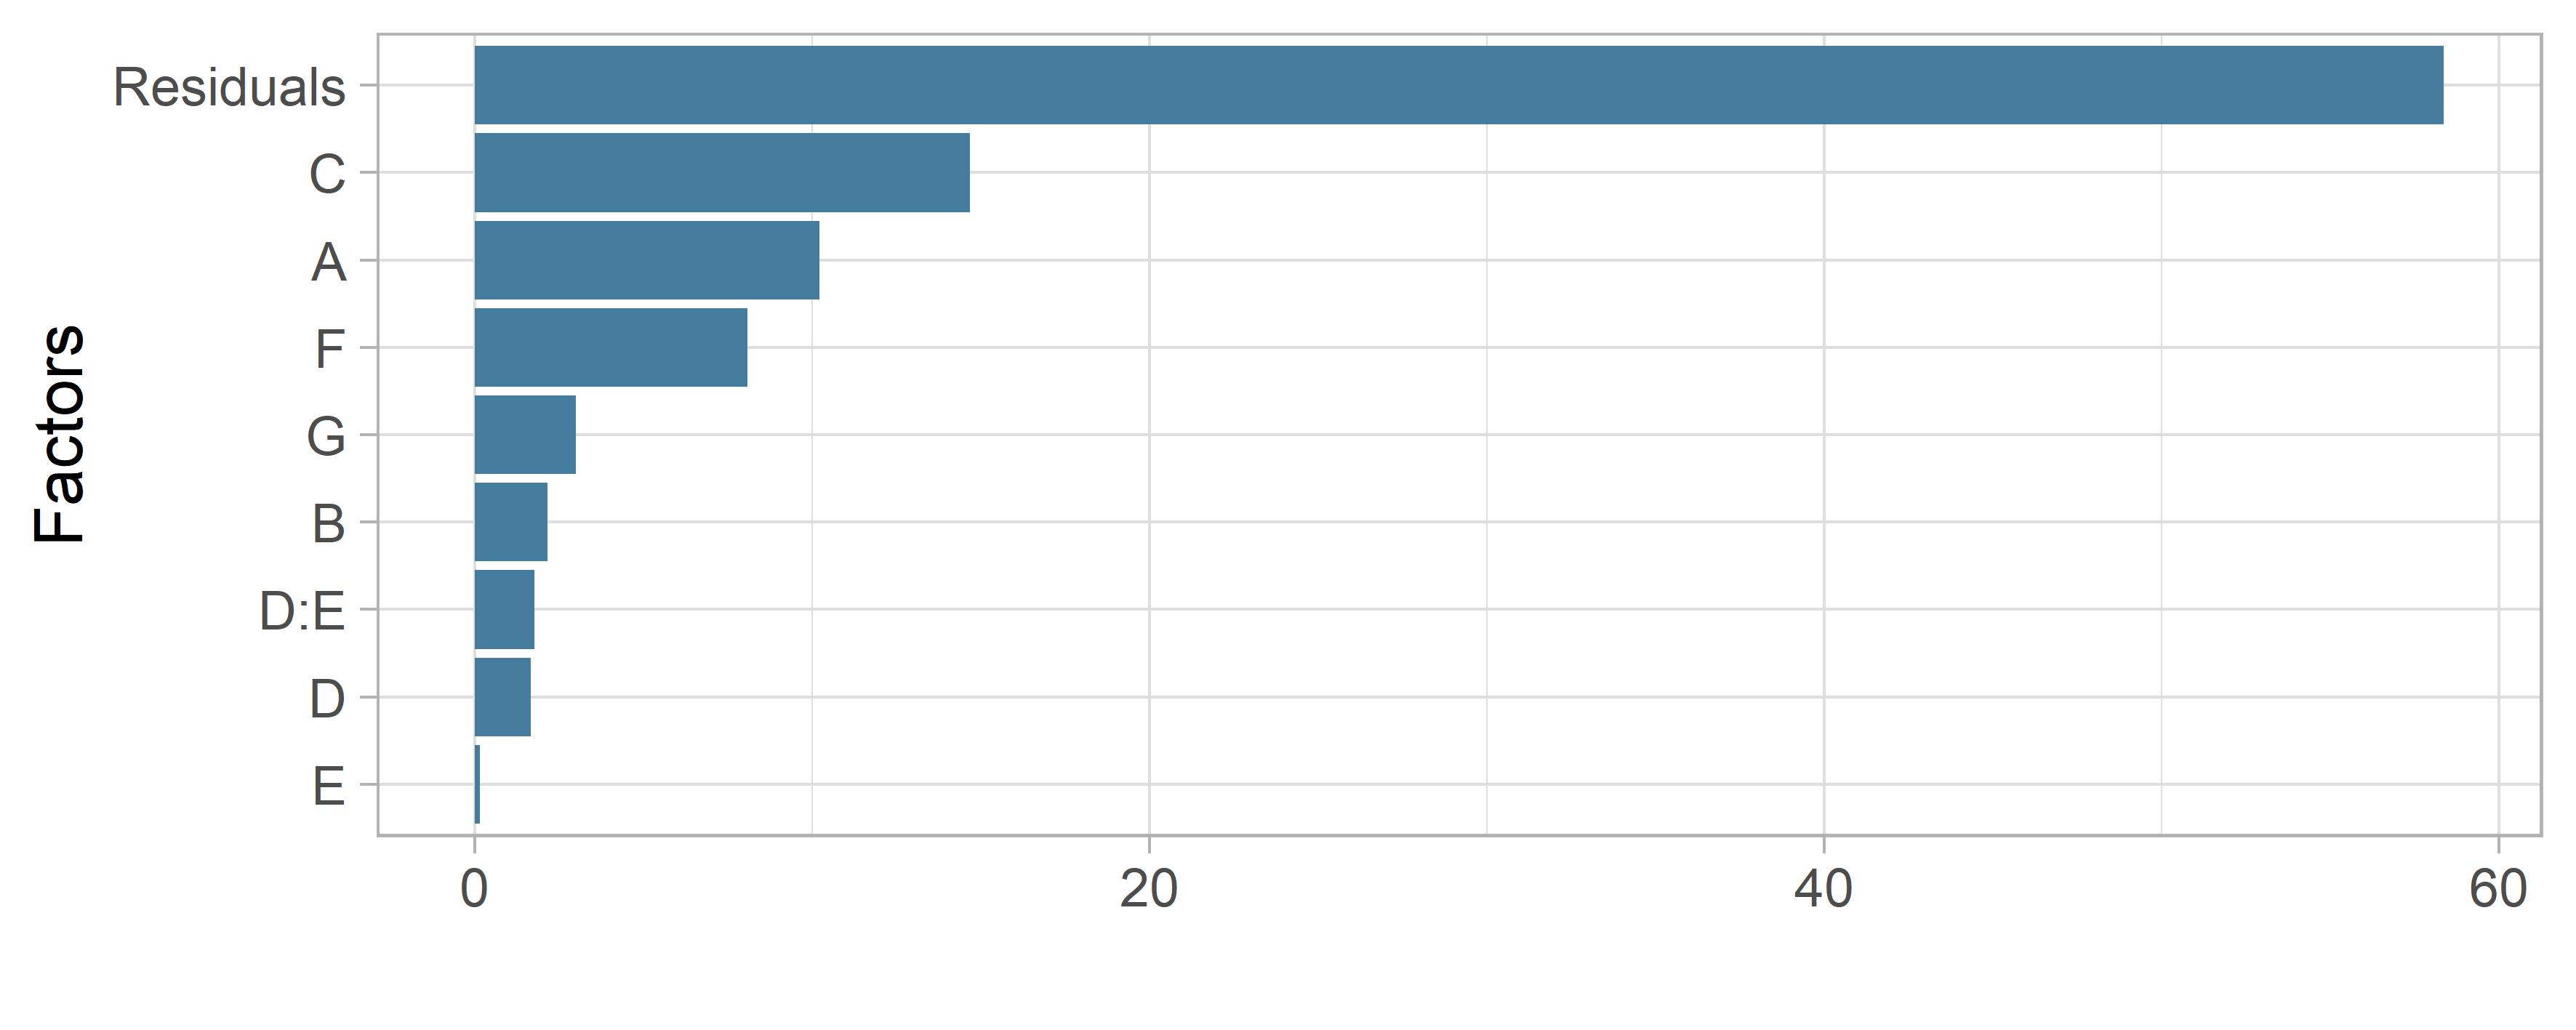
\includegraphics[width=1\linewidth]{simulations/taguchi/plots/percentage_contribution}
	\caption{percentage contribution}
	\label{fig:hyperparam_tuning:percentage_contribution}
\end{figure}

\subsubsection{Main-effects and interaction chart}
Identifying the optimal conditions needs analysis of the main effects per factor. They allow to predict the levels that lead to the best result~\cite{roy_primer_1990}.

\begin{quote}
	\begin{em}
		\enquote{The main-effects chart is a plot of average responses at different levels of a factor versus the factor levels.}~\cite{yang_design_2009}
	\end{em}
\end{quote}

For every factor, the mean of all results per level is summed up and subsequently divided by the number of runs per level. The resulting main-effect charts are visualized in Figure \ref{fig:hyperparam_tuning:main_effects}.

\begin{figure}[ht] 
	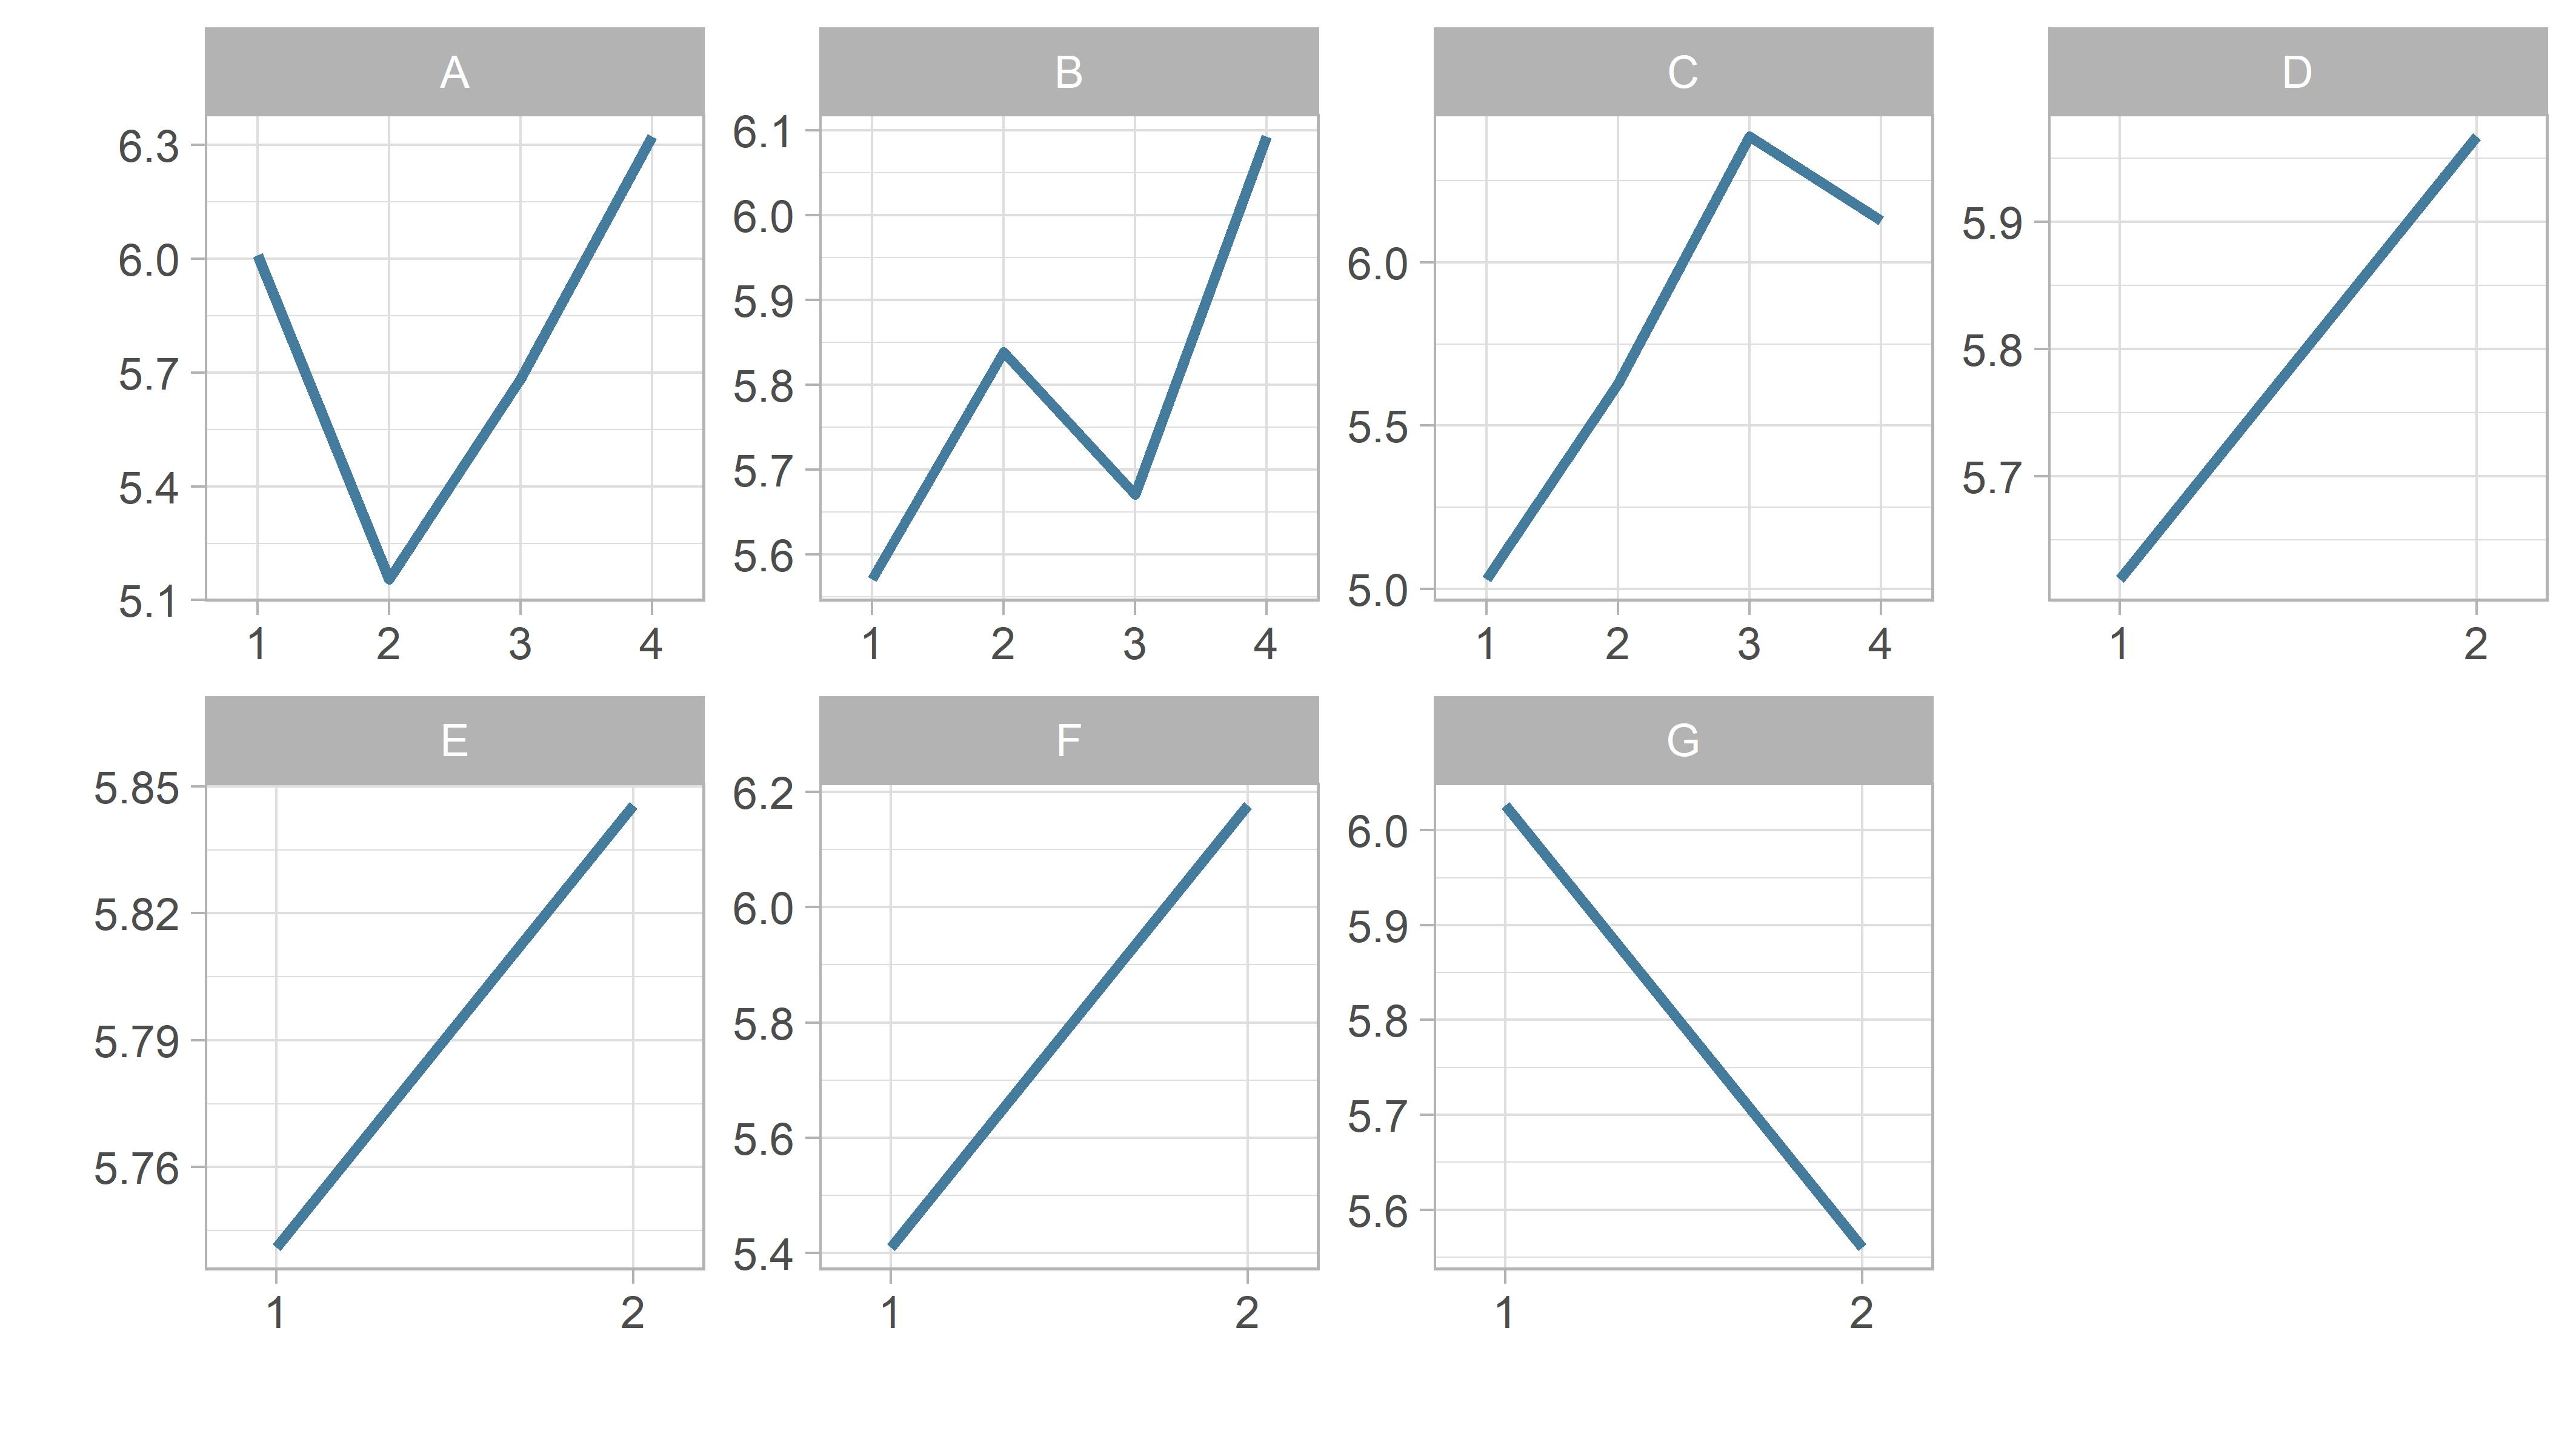
\includegraphics[width=1\linewidth]{simulations/taguchi/plots/main_effects}
	\caption{Main Effects}
	\label{fig:hyperparam_tuning:main_effects}
\end{figure}


In case there is no interaction, the optimal setting is easily determined by using the main effects chart. Go over every factor in the chart and use the best level (in this experiment, the level with the highest value). If interactions, however, exist, they might have an influence on the best settings and need further investigation~\cite{yang_design_2009}. The previously defined interaction is visualized in an interaction plot in Figure \ref{fig:hyperparam_tuning:interaction_plot}. The calculation is similar to calculating main effects can be seen in Equation \todo{Show calculation example for DE}.

\begin{figure}[ht] 
	\centering
	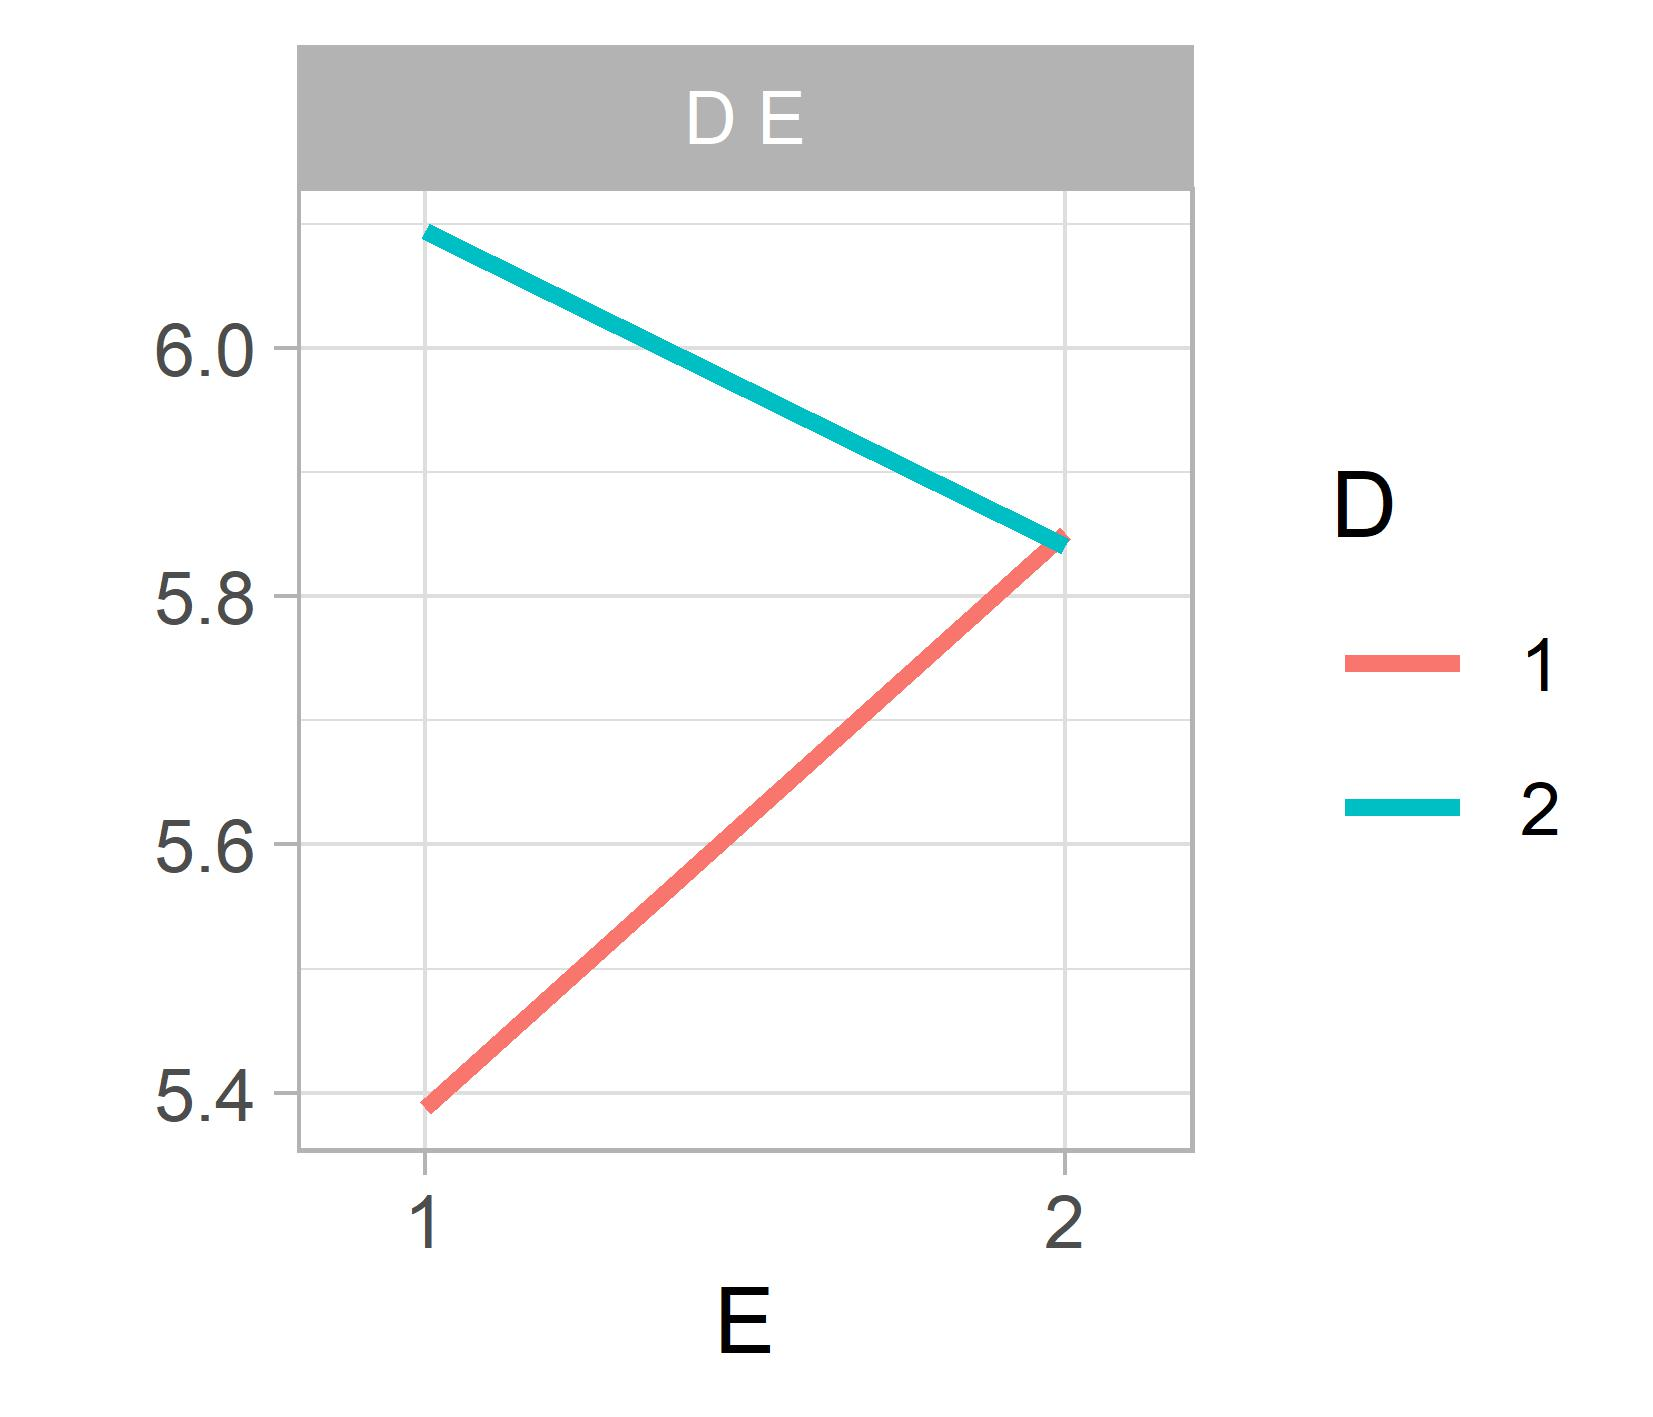
\includegraphics[width=0.4\linewidth]{simulations/taguchi/plots/test_of_interaction}
	\caption{interaction plot}
	\label{fig:hyperparam_tuning:interaction_plot}
\end{figure}

The crossing of lines in the interaction plot indicates that an interaction between the two factors might exist~\cite{field_discovering_2012}. The more parallel the lines are, the less likely an interaction. The magnitude of the angle between the lines corresponds to the degree of interaction presence~\cite{roy_primer_1990}.

\subsubsection{Selection of optimal setting}
When choosing the optimal setting, the first step is to look at the best main effects combination. For this experiment, the best combination according the main effects is the following: $A_4$, $B_4$, $C_3$, $D_2$, $E_2$, $F_2$, $G_1$.

Analysing the interaction graph and the ANOVA table, the interaction D:E however might be significant. The interaction plot in Figure \ref{fig:hyperparam_tuning:interaction_plot} suggest $D_2$ and $E_1$ as the best combination. This is optimal, as $D_2$ is also recommended by the main effects. While $E_1$ does not correspond to its main effect, the low F value of the factor E suggests low significance anyway. Concluding this line of thought, the combination $A_4$, $B_4$, $C_3$, $D_2$, $E_1$, $F_2$, $G_1$ is preferred.

\paragraph{Optimum performance calculation}
\label{sect:hyperparameter_tuning:optimum_perf_caluclation}
To calculate the predicted results of a genetic algorithm with these settings, optimal performance calculation can be applied. Equation \ref{equ:hyperparameter_tuning:optimum_perf_main_effect}, which incorporates only the suggested main effects, and Equation \ref{equ:hyperparameter_tuning:optimum_perf_included_interaction}, which includes the additional interaction term D:E. The calculation formulas are sourced from Roy~\cite{roy_primer_1990}.

\begin{equation}
	\begin{split}
		Y_{opt} &= \overline{T} + (\overline{A_4} - \overline{T}) + (\overline{B_4} - \overline{T}) + (\overline{C_3} - \overline{T}) + (\overline{D_2} - \overline{T}) + \\& (\overline{E_2} - \overline{T}) + (\overline{F_2} - \overline{T}) + (\overline{G_1} - \overline{T}) \\
			&= 8.06
	\end{split}
	 \label{equ:hyperparameter_tuning:optimum_perf_main_effect}
\end{equation}


\begin{equation}
	\begin{split}
		Y_{opt} &= \overline{T} + (\overline{A_4} - \overline{T}) + (\overline{B_4} - \overline{T}) + (\overline{C_3} - \overline{T}) + (\overline{D_2} - \overline{T}) + \\& (\overline{E_1} - \overline{T})  + ([\overline{DxE}]_2 - \overline{T})  + (\overline{F_2} - \overline{T}) + (\overline{G_1} - \overline{T}) \\
		&= 8.13
	\end{split}
	 \label{equ:hyperparameter_tuning:optimum_perf_included_interaction}
\end{equation}

The inclusion of the interaction term D:E results in an improved performance estimation from 8.06 to 8.13. Consequently, the final optimal combination of control parameters is determined as follows: CrossoverType: Uniform 0.5, CrossoverRate: 0.9, MutationRate: 0.3, ChromosomeType: Time+NPC, GeneType: Integer, TournamentSize: 4 and IndividualMutationRate: 0.1.

The added higher granularity for the crossover function was preferred, which is provided by the chromosome encoding 'Time+NPC'. This encoding allows for the crossover operation to exchange actions between actors across different time steps. Notably, the choice of Uniform 0.5 as the CrossoverType as well as the high CrossoverRate and MutationRate is surprising. It remains to be seen, if the genetic algorithms will behave similar to random search or if the high rates will contribute to maintain diversity in its population.

\subsubsection{Signal-to-Noise Ratio}
As discussed earlier, the ANOVA model has a high error, which suggests high randomness. Taguchi recommends using signal-to-noise ratio (S/N) to reduce the variability, as using only the mean of the results (which is used when calculating the main effects) does not take the variation into account~\cite{roy_primer_1990}.\todo{Explain signal to noise in one sentence} Essentially, a higher signal-to-noise ratio corresponds to reduced variance.

\begin{quote}
	\begin{em}
		\enquote{The use of the S/N ratio offers an objective way to look at the two characteristics (consistency and average value) together.}~\cite{roy_primer_1990}
	\end{em}
\end{quote}

S/N is calculated in two steps~\cite{roy_primer_1990}. The first step involves determining  the mean square deviation (MSD). Depending on the quality characteristic, a different equation has to be chosen. In this scenario, a higher result is better, thus Equation \ref{equ:hyperparam_tuning:MSD} is used for each repetition, with $y_1$ being the result of repetition 1 and $n$ the number of repetitions. The signal-to-noise ratio is calculated in the second step in Equation \ref{equ:hyperparam_tuning:S_N}.

\begin{equation}
	\begin{split}
		MSD & = (1/y^2_1 + 1/y^2_2 + 1/y^2_3 + ... ) / n
	\end{split}
	 \label{equ:hyperparam_tuning:MSD}
\end{equation}

\begin{equation}
	\begin{split}
		S/N & = -10 log_{10} (MSD)
	\end{split}
	 \label{equ:hyperparam_tuning:S_N}
\end{equation}

Generating the main effects and performing ANOVA is done using the S/N instead. As a side note, it's important to mention that only 15 DOF are available for the ANOVA analysis, as repetitions per run are merged when calculating S/N, which can be observed in Equation \ref{equ:hyperparam_tuning:S_N_anova_DOF}.

\begin{equation}
	\begin{split}
		DOF & = totalNumberOfResults - 1 \\
		& = numberOfTrials * 1 - 1 \\
		& = 16 - 1 = 15
	\end{split}
	 \label{equ:hyperparam_tuning:S_N_anova_DOF}
\end{equation}

\begin{table}[ht]
	\centering
	\begin{tabular}{lrrrrr}
		\hline
		& Df & Sum Sq & Mean Sq & F value & Pr($>$F) \\ 
		\hline
		A & 3 & 5.14 & 1.71 & 3.54 & 0.3682 \\ 
		B & 3 & 2.04 & 0.68 & 1.40 & 0.5397 \\ 
		C & 3 & 10.59 & 3.53 & 7.28 & 0.2644 \\ 
		D & 1 & 1.29 & 1.29 & 2.67 & 0.3498 \\ 
		E & 1 & 0.39 & 0.39 & 0.81 & 0.5329 \\ 
		F & 1 & 4.43 & 4.43 & 9.15 & 0.2033 \\ 
		G & 1 & 2.28 & 2.28 & 4.70 & 0.2751 \\ 
		D:E & 1 & 0.92 & 0.92 & 1.89 & 0.4005 \\ 
		Residuals & 1 & 0.48 & 0.48 &  &  \\ 
		\hline
	\end{tabular}
	\caption{S/N ANOVA results}
	\label{tab:hyperparameter_tuning:s_n_anova_results}
\end{table}

Based on the p values obtained from the ANOVA results in Table \ref{tab:hyperparameter_tuning:s_n_anova_results}, no factor shows statistical significance to reject the null hypothesis, which states that a factor has no significant effect. Considering this fact, further investigations were deemed unnecessary. The often recommend signal-to-noise ratio does not appear suitable for this experiment, thus the previously calculated settings in Paragraph \ref{sect:hyperparameter_tuning:optimum_perf_caluclation} will remain unchanged.

\subsubsection{Elite Selection}
Although the optimal hyperparameter setting are reviewed in Chapter \ref{chap:evaluation}, a problem was obvious when analysing results of a GA using the settings from Section \ref{sect:hyperparameter_tuning:optimum_perf_caluclation}. Setbacks in the fitness value between two generations happen frequently, likely due to the high crossover and mutation rates. In order to mitigate this problem, elite selection with a size of 2 was implemented. Per generation, the two best individuals are now copied into the next generation without modifications, which makes worse performance between generations not possible. It is important to note, that these two individuals can still be selected by tournament selection for modification, its just that a copy of them is automatically saved. Figure \ref{fig:hyperparameter_tuning:elite_no_elite_comp} compares both no elite selection with an elite selection of 2. For a few selected repetitions, the best individual fitness per generation is plotted.

\begin{figure}[ht] 
	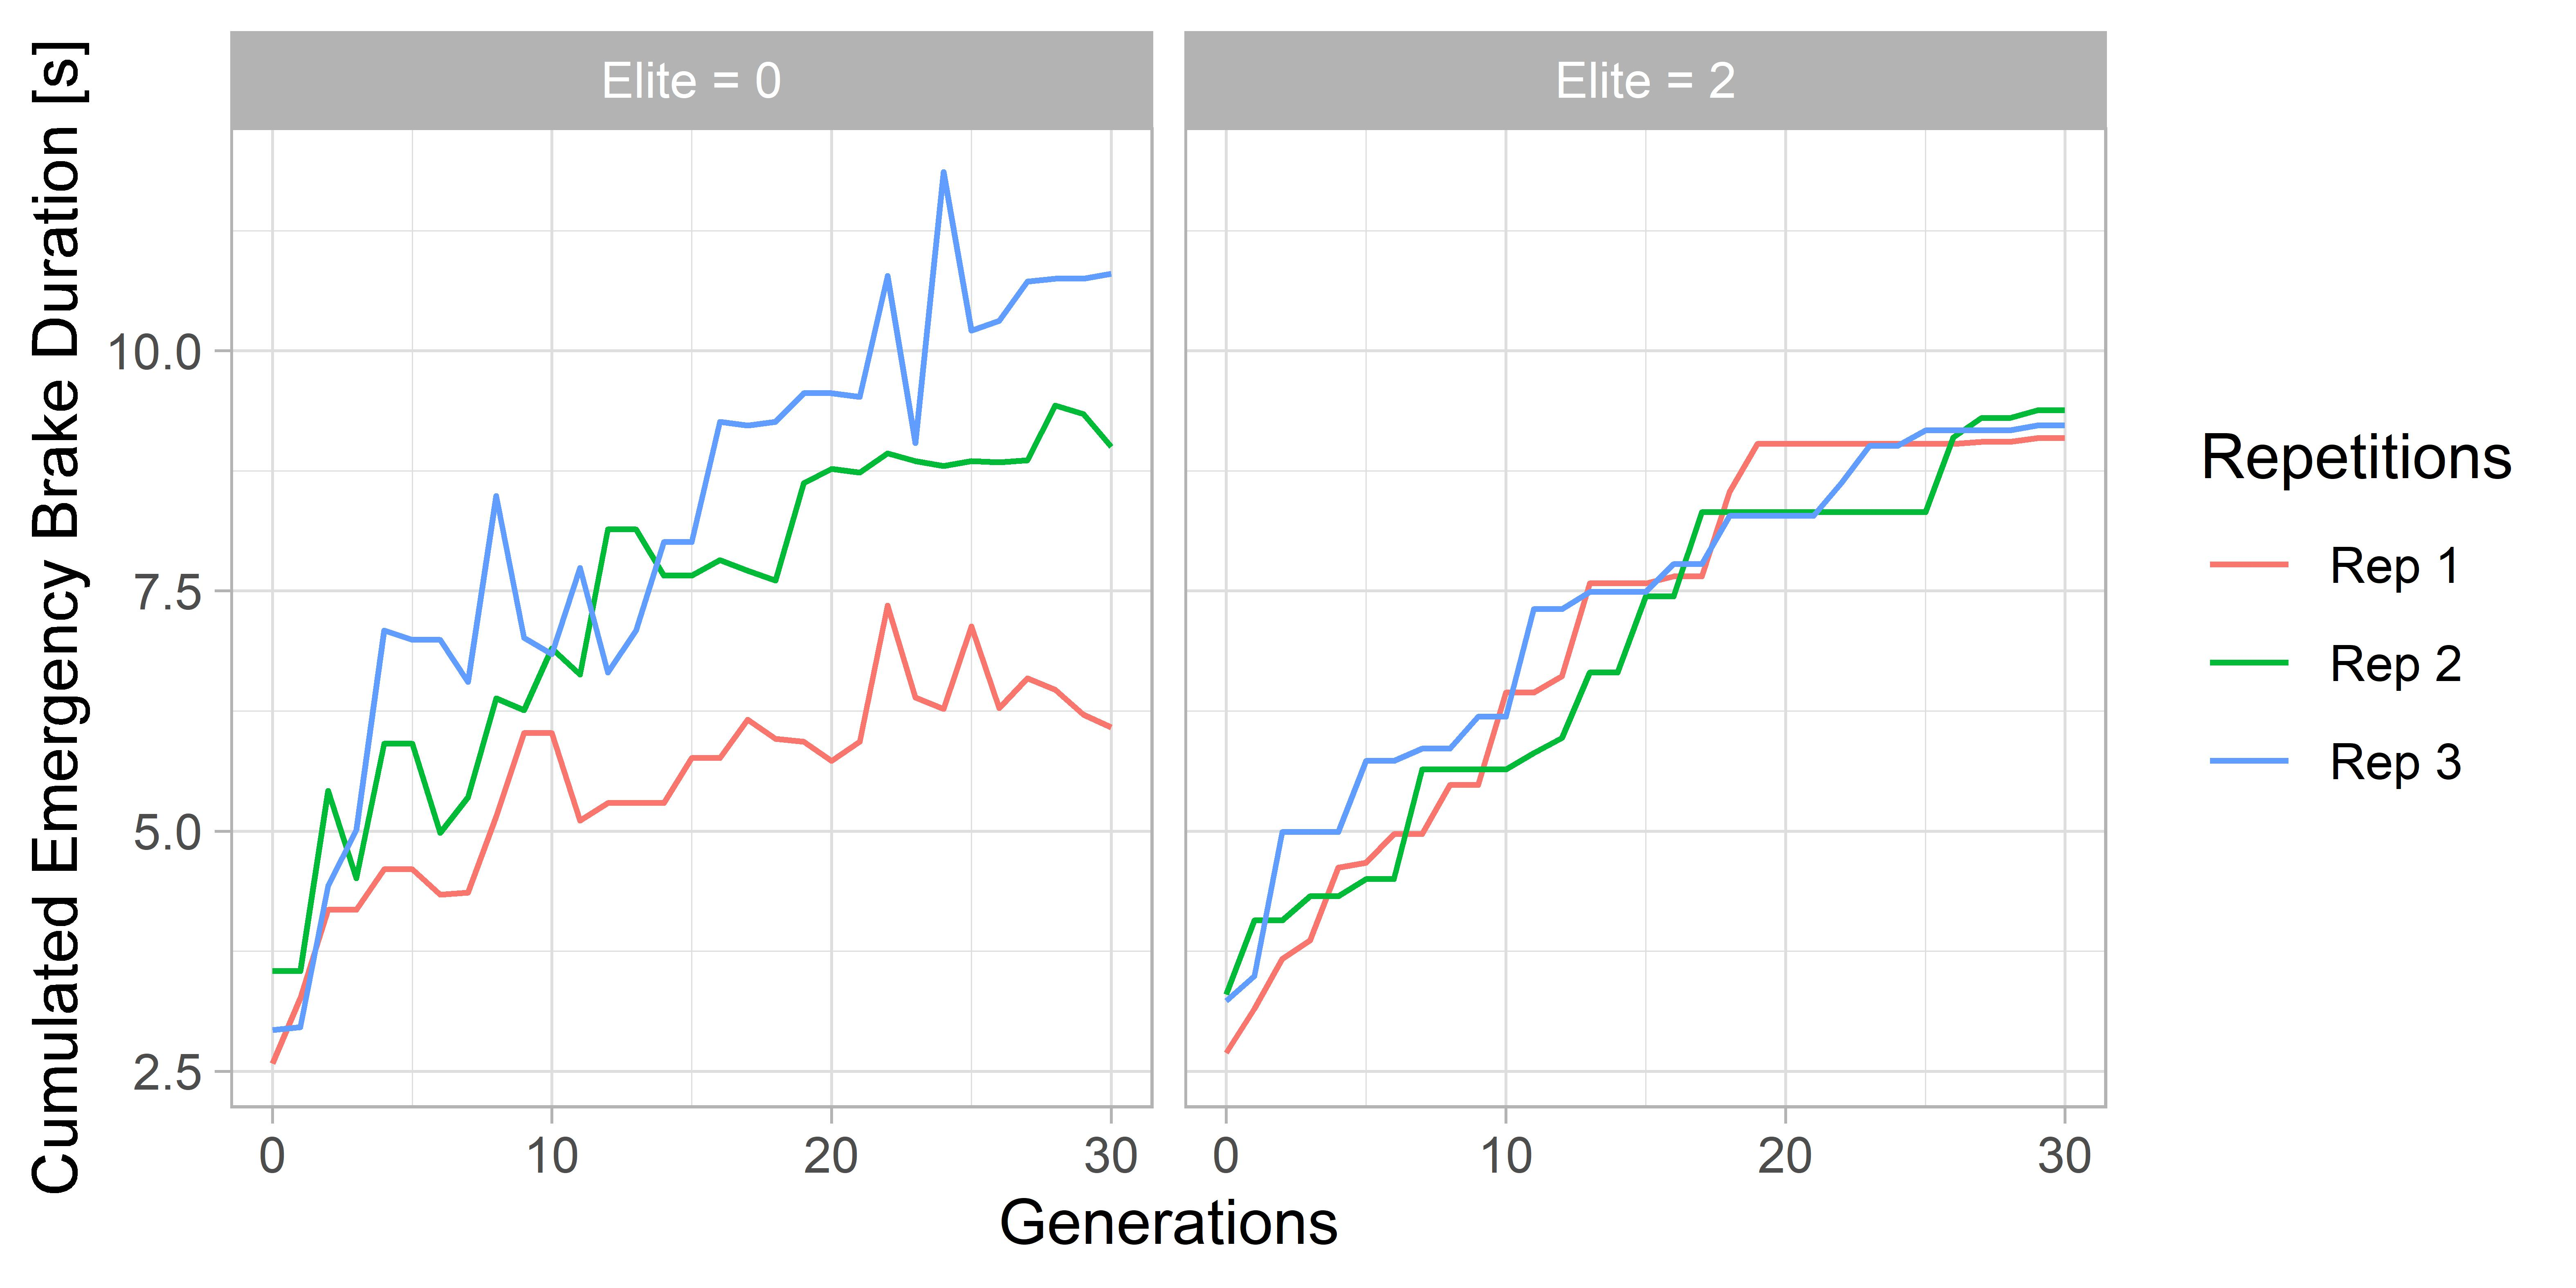
\includegraphics[width=1\linewidth]{simulations/evaluation/plots/elite_vs_no_elite_generations}
	\caption{elite selection comparison over GA generations}
	\label{fig:hyperparameter_tuning:elite_no_elite_comp}
\end{figure}

For analysing the statistical significance in the differences in mean between a genetic algorithm using elite selection of 2 vs no elite selection, a t-test can be used. To account for possible violation of the assumption of homogeneity, a robust welch's t-test is applied, which adjusts the DOF accordingly~\cite{field_discovering_2012}. On average, using elite improved the performance (M = 8.52, SE = 0.31), compared to using no elite (M = 7.92, SE = 0.55). This difference was not significant \textit{t}(14.21) = 0.96, p > 0.05; however, it did represent a small-sized effect r = 0.25. A visual comparison of both GAs, each repeated 10 times, can be seen in Figure \ref{fig:hyperparameter_tuning:elite_comparison}. Due to the existence of the aforementioned small effect as well as the reduced variance, it is concluded that elite selection of 2 is added to the settings from \ref{sect:hyperparameter_tuning:optimum_perf_caluclation}, which will be used in Chapter \ref{chap:evaluation}.

\begin{figure}[ht] 
	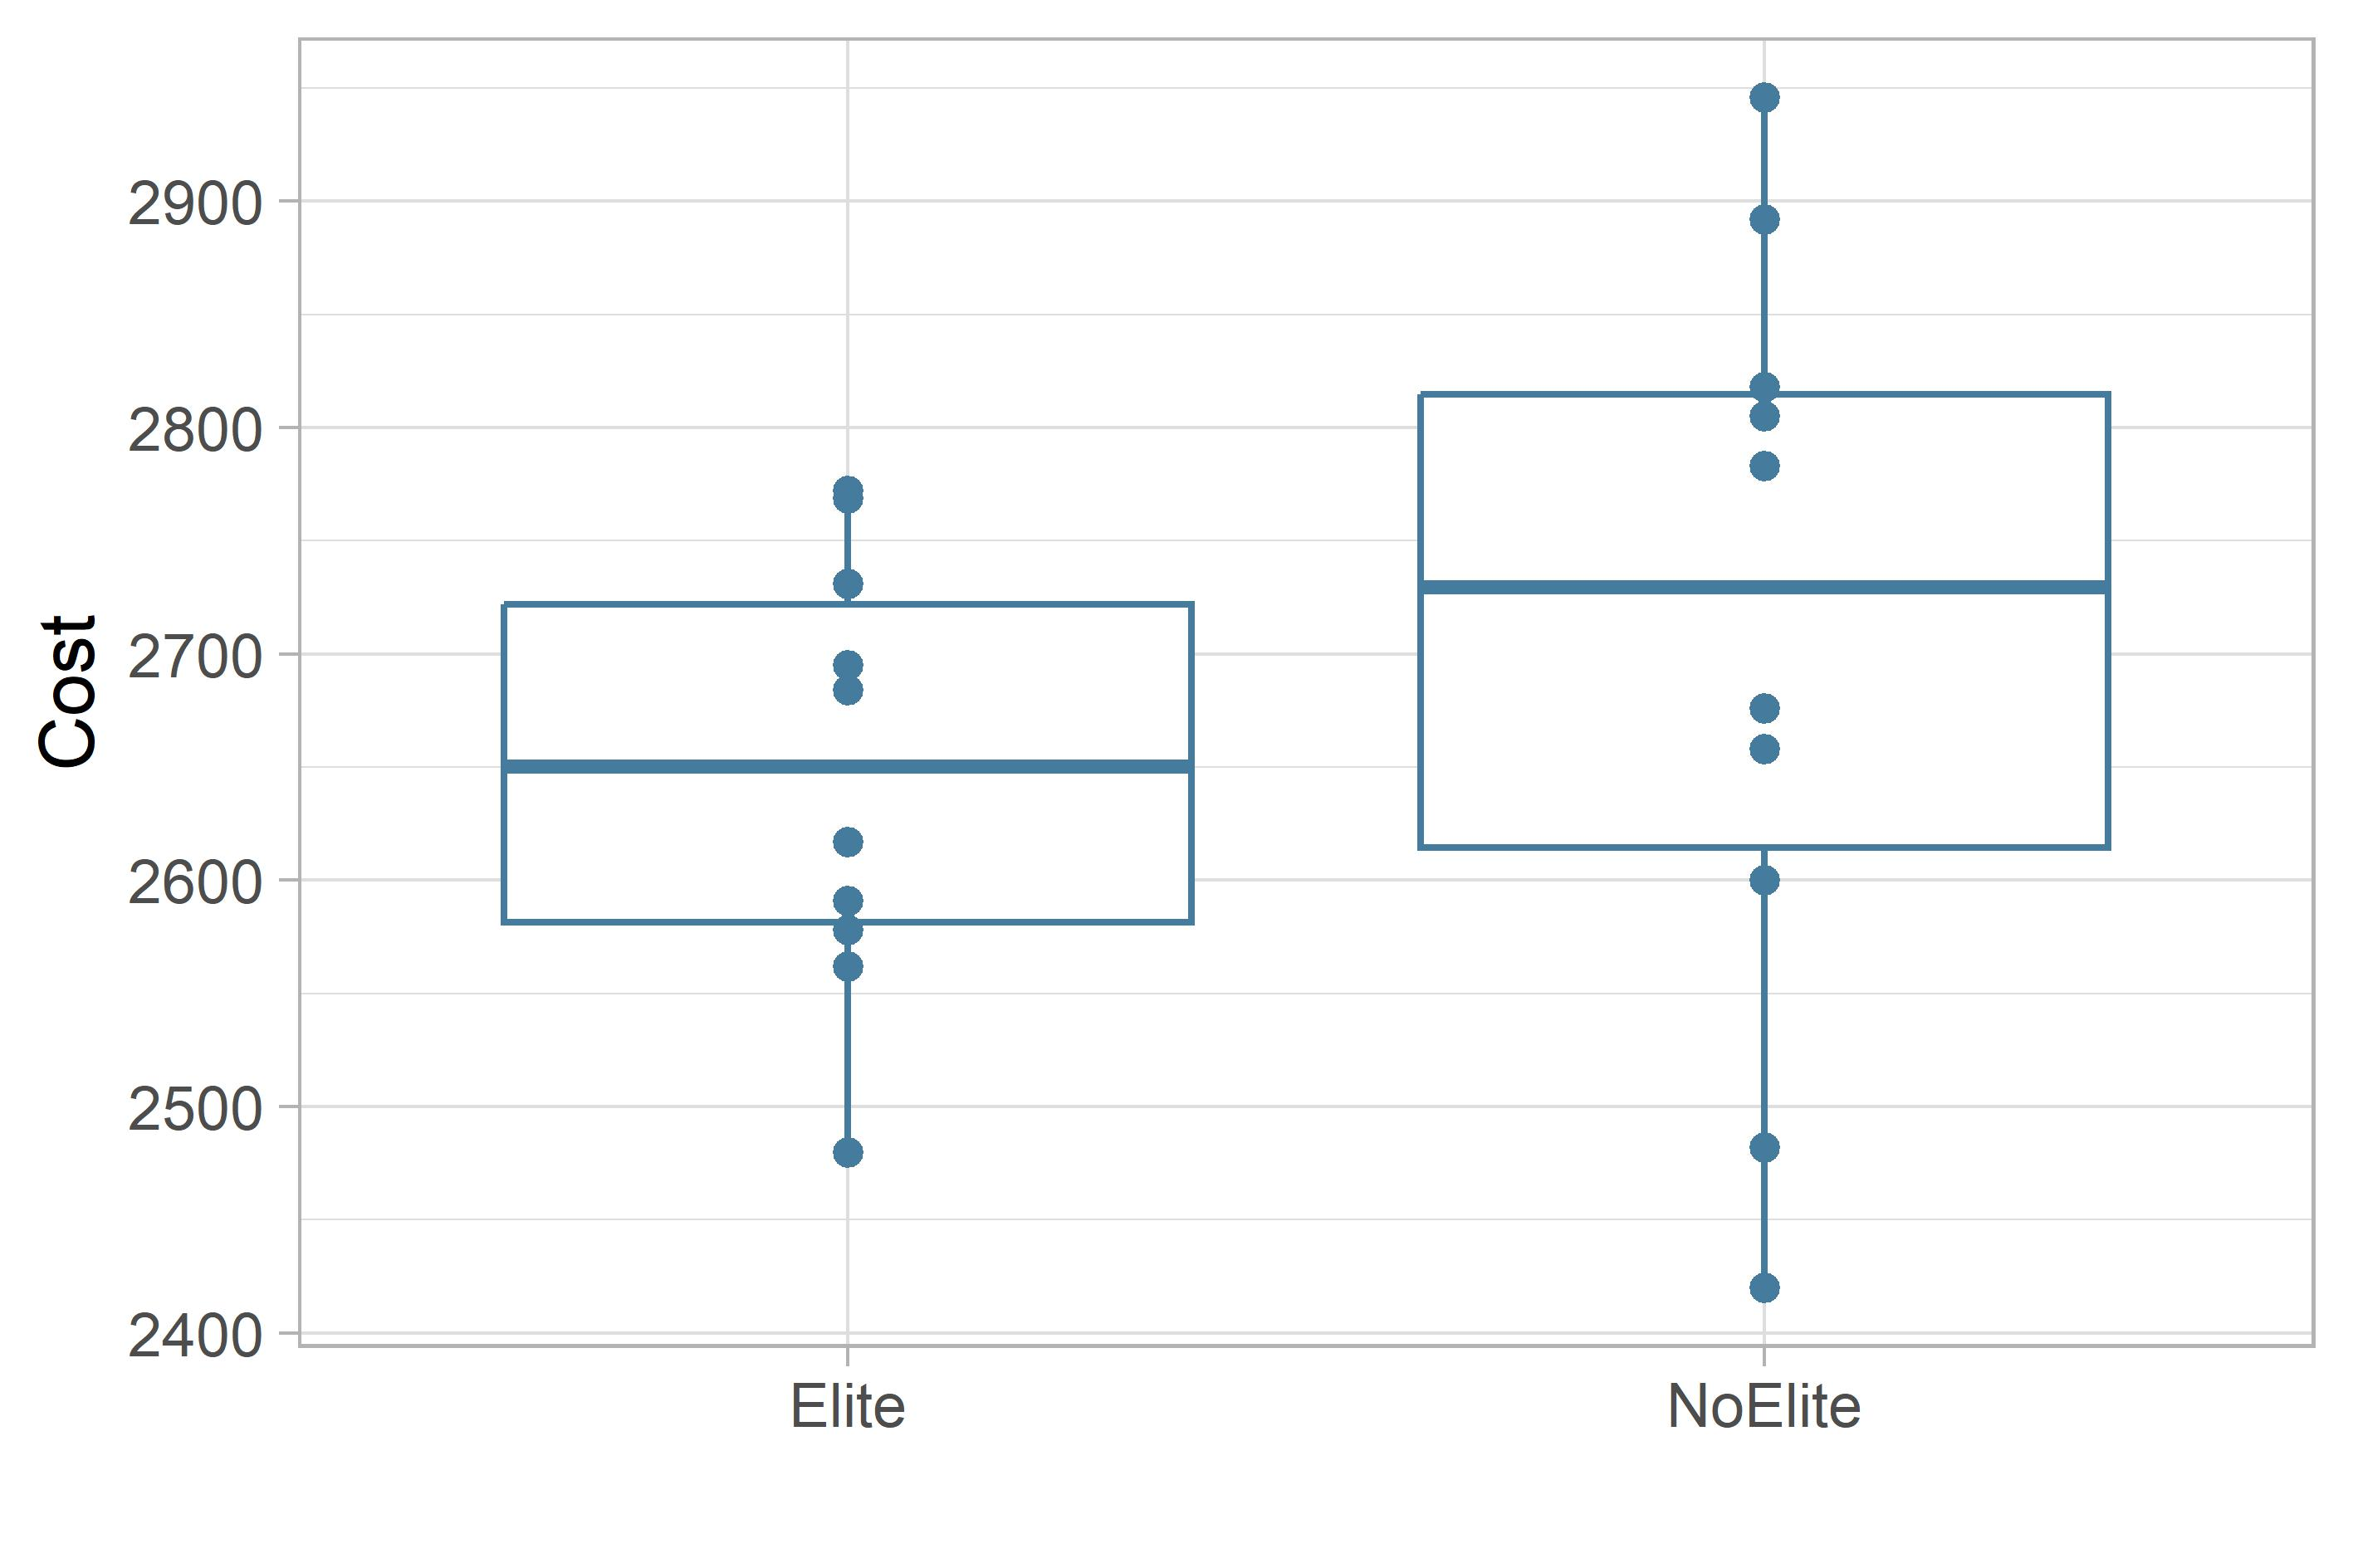
\includegraphics[width=1\linewidth]{simulations/evaluation/plots/elite_vs_no_elite}
	\caption{elite selection comparison results}
	\label{fig:hyperparameter_tuning:elite_comparison}
\end{figure}

\paragraph{Effect Size}
According to Field et al.~\cite{field_discovering_2012} effect sizes provide an objective measure on the importance of an effect, where 0 means no effect and 1 means a perfect effect. They allow for a standardized measure and are not affected by sample size. He further recommends to utilize the widely used suggestions made by Cohen~\cite{cohen_statistical_1988, cohen_power_1992} on defining between a large or small effect:

\begin{itemize}
	\item r = .10 (small effect): The effect explains 1\% of the variance. 
	\item r = .30 (medium effect): The effect explains 9\% of the variance. 
	\item r = .50 (large effect): The effect explains 25\% of the variance.
\end{itemize} 

Effect sizes also be used to compare different algorithms in Chapter \ref{chap:evaluation} as well and are calculated for a t-test using Equation \ref{equ:hyperparameter_tuning:effect_size}.

\begin{equation}
	\begin{split}
		r & = \sqrt{\frac{t^2}{t^2 + DOF}}
	\end{split}
	 \label{equ:hyperparameter_tuning:effect_size}
\end{equation}





\chapter{Evaluation}
\label{chap:evaluation}
This Chapter will compare the GA settings proposed in \ref{sect:hyperparameter_tuning:optimum_perf_caluclation} with the best settings found in \ref{sect:hyperparameter_tuning:population} as well as with random search. The three different algorithms that are going to be compared are as follows:
\begin{itemize}
	\item \textbf{Default} Genetic Algorithm - using the best settings found in \ref{sect:hyperparameter_tuning:population}
	\begin{itemize}
		\item CrossoverType: Two-Point, CrossoverRate: 0.8, MutationRate: 0.20, TournamentSize: 4, ChromosomeType: Time, GeneType: Integer, IndividualMutatioRate: 0.1 and EliteSelection: 0. 
		\item The algorithm will be run 10 times. The population of 96 needs to be simulated 31 times per run (30 generations + initialization), which leads to $96 * 31 * 10 = 29,760$ simulations.
	\end{itemize}
	\item \textbf{Optimized} Genetic Algorithm - using the recommended settings found in \ref{sect:hyperparameter_tuning:optimum_perf_caluclation}
	\begin{itemize}
		\item CrossoverType: Uniform 0.5, CrossoverRate: 0.9, MutationRate: 0.3, ChromosomeType: Time+NPC, GeneType: Integer, TournamentSize: 4 and IndividualMutationRate: 0.1 and EliteSelection: 2. 
		\item The algorithm will be run 10 times. The population of 96 needs to be simulated 31 times per run (30 generations + initialization), which leads to $96 * 31 * 10 = 29,760$ simulations.
	\end{itemize}
	\item \textbf{Random} Search
	\begin{itemize}
		\item Randomly choosing actions, using the probabilities from Table \ref{tab:implementation:action_probabilities}. 
		\item The algorithm will be run 10 times each with $2,976$ simulations, always taking the maximum value as the result. $29,760$ simulations were executed in total.
	\end{itemize}
\end{itemize}


The evaluation is done over 4 different start scenarios which can be found at the Appendix \ref{chap:appendix_a}.

\section{Start Scenario 1}
First, a comparison of the three algorithms on start scenario 1 was made. This is the same start scenario, that was used in Chapter \ref{chap:hyperparameter_tuning}. The results are shown in Figure \ref{fig:evaluation:sim_1_comparison}.

\begin{figure}[ht] 
	\label{fig:evaluation:sim_1_comparison}
	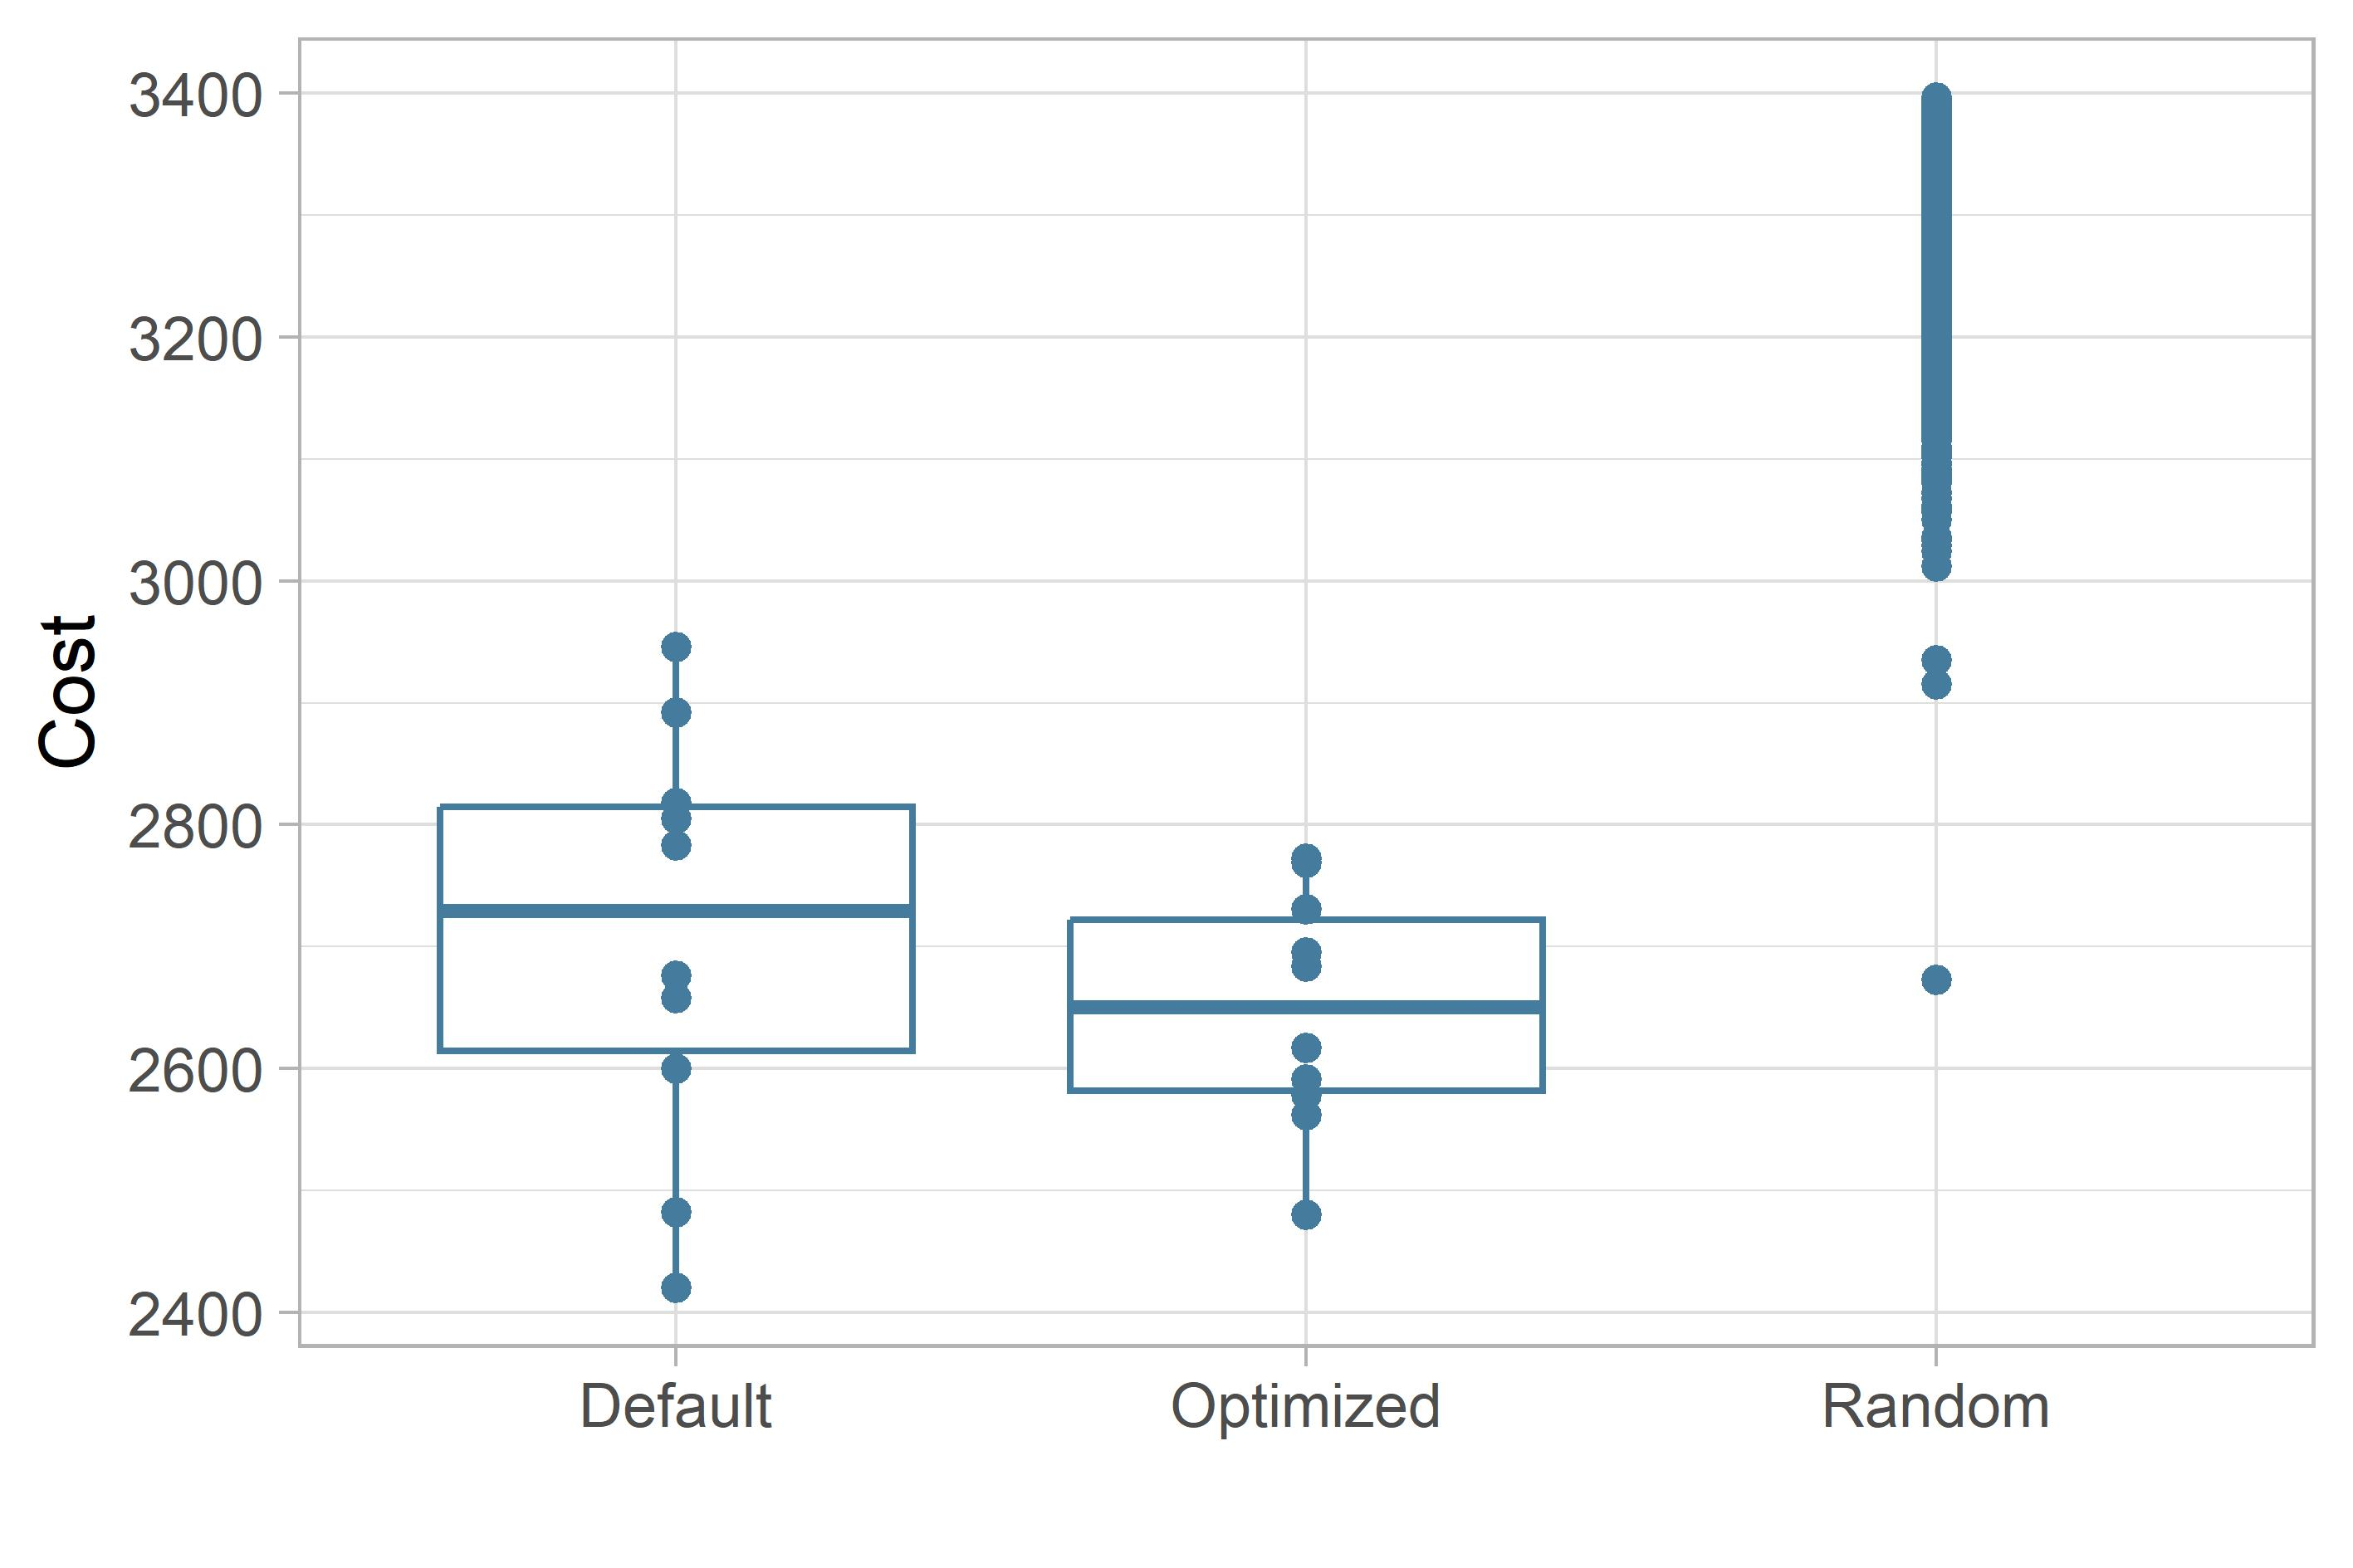
\includegraphics[width=1\linewidth]{simulations/evaluation/plots/sim_1_comparison}
	\caption{Start Scenario 1: Default GA vs Optimized GA vs Random Search}
\end{figure}

Analysing the graph, the Optimized GA clearly outperformed the Default GA as well as Random Search. Welchs t-test shows that on average, greater fitness is achieved by using Optimized GA (M = 8.52, SE = 0.31) than from using Default GA (M = 7.09, SE = 0.34). This difference was significant \textit{t}(17.87) = 3.15, p < .01. It did represent a large effect r = 0.60.
Compared to Random (M = 4.943, SE = 0.4), the Optimized GA has even higher dominance, with a significant difference \textit{t}(16.9) = 7.12, p < .001 and a large effect r = 0.87. The better performance of the Optimized GA was however unsurprising, as it was specifically trained on the used start scenario.

To further analyse both genetic algorithms, a look at their performance over the generations next to their diversity chart is of interest. Figure \ref{fig:evaluation:sim_1_ga_comparison} plots the mean over 10 repetitions, the outline show the first and third quantiles.

\begin{figure}[ht] 
	\label{fig:evaluation:sim_1_ga_comparison}
	\begin{minipage}[b]{0.5\linewidth}
		\centering
		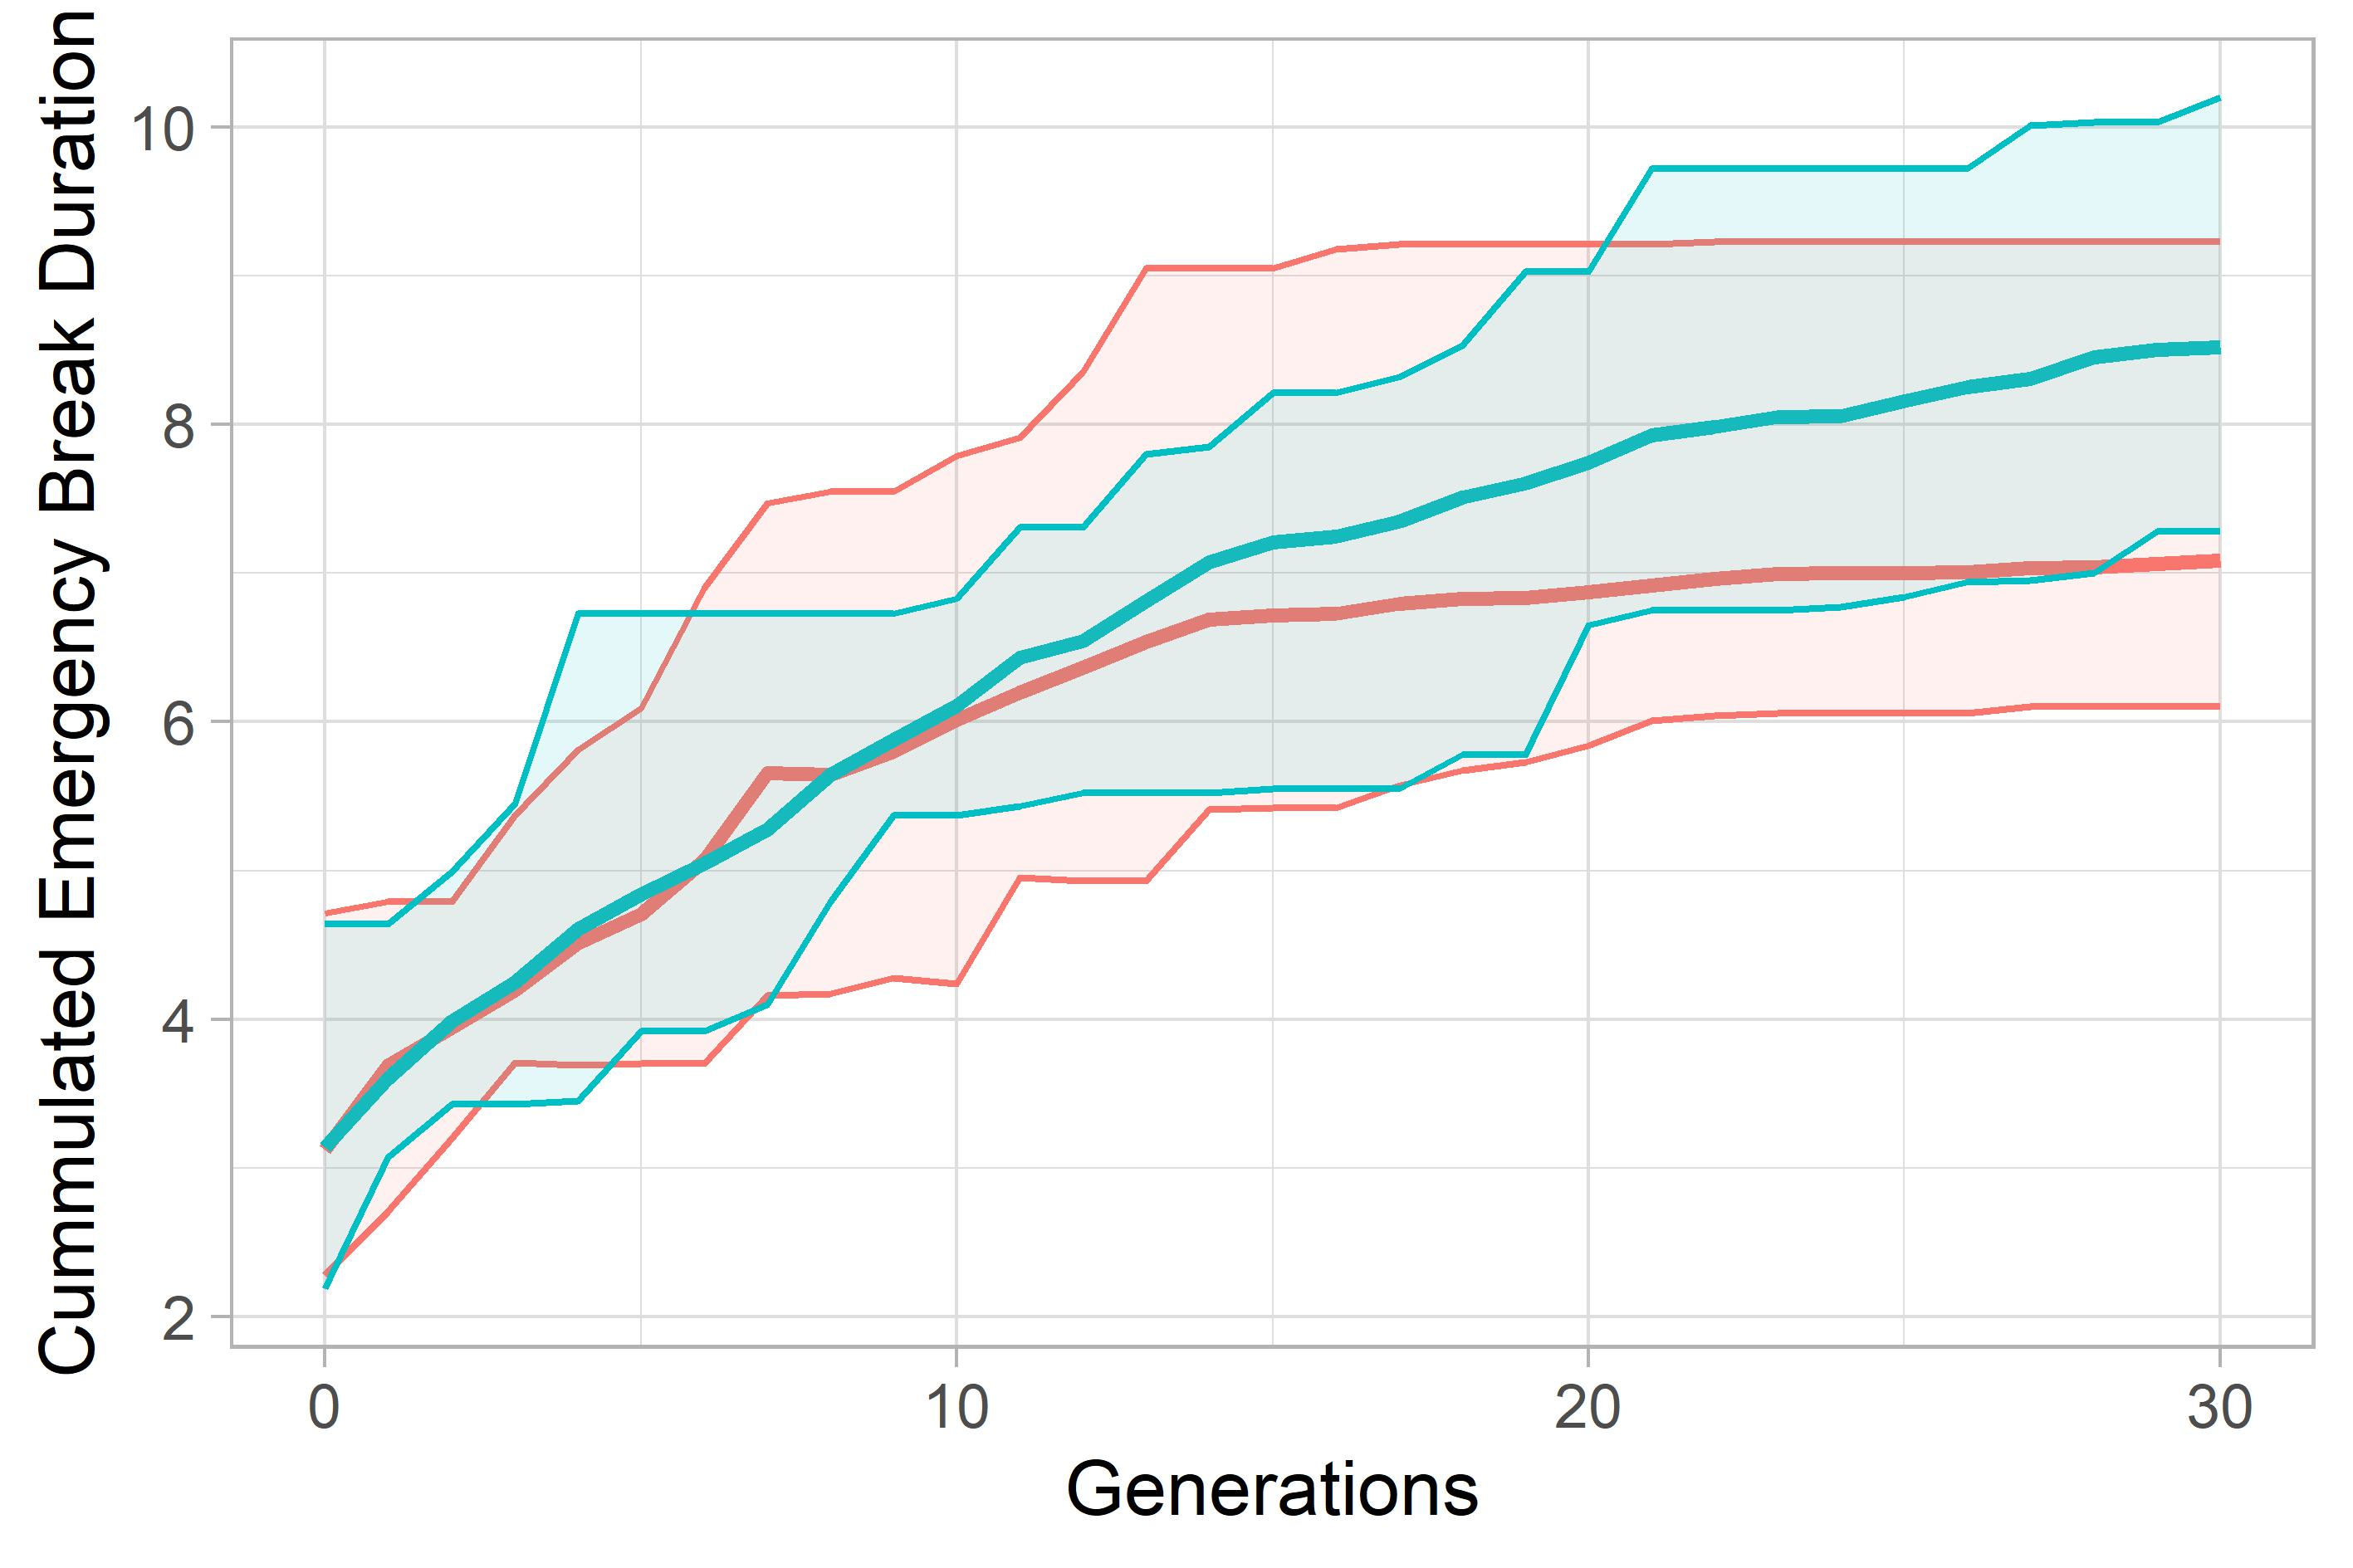
\includegraphics[width=1\linewidth]{simulations/evaluation/plots/sim_1_ga_generations} 
	\end{minipage}%%
	\begin{minipage}[b]{0.5\linewidth}
		\centering
		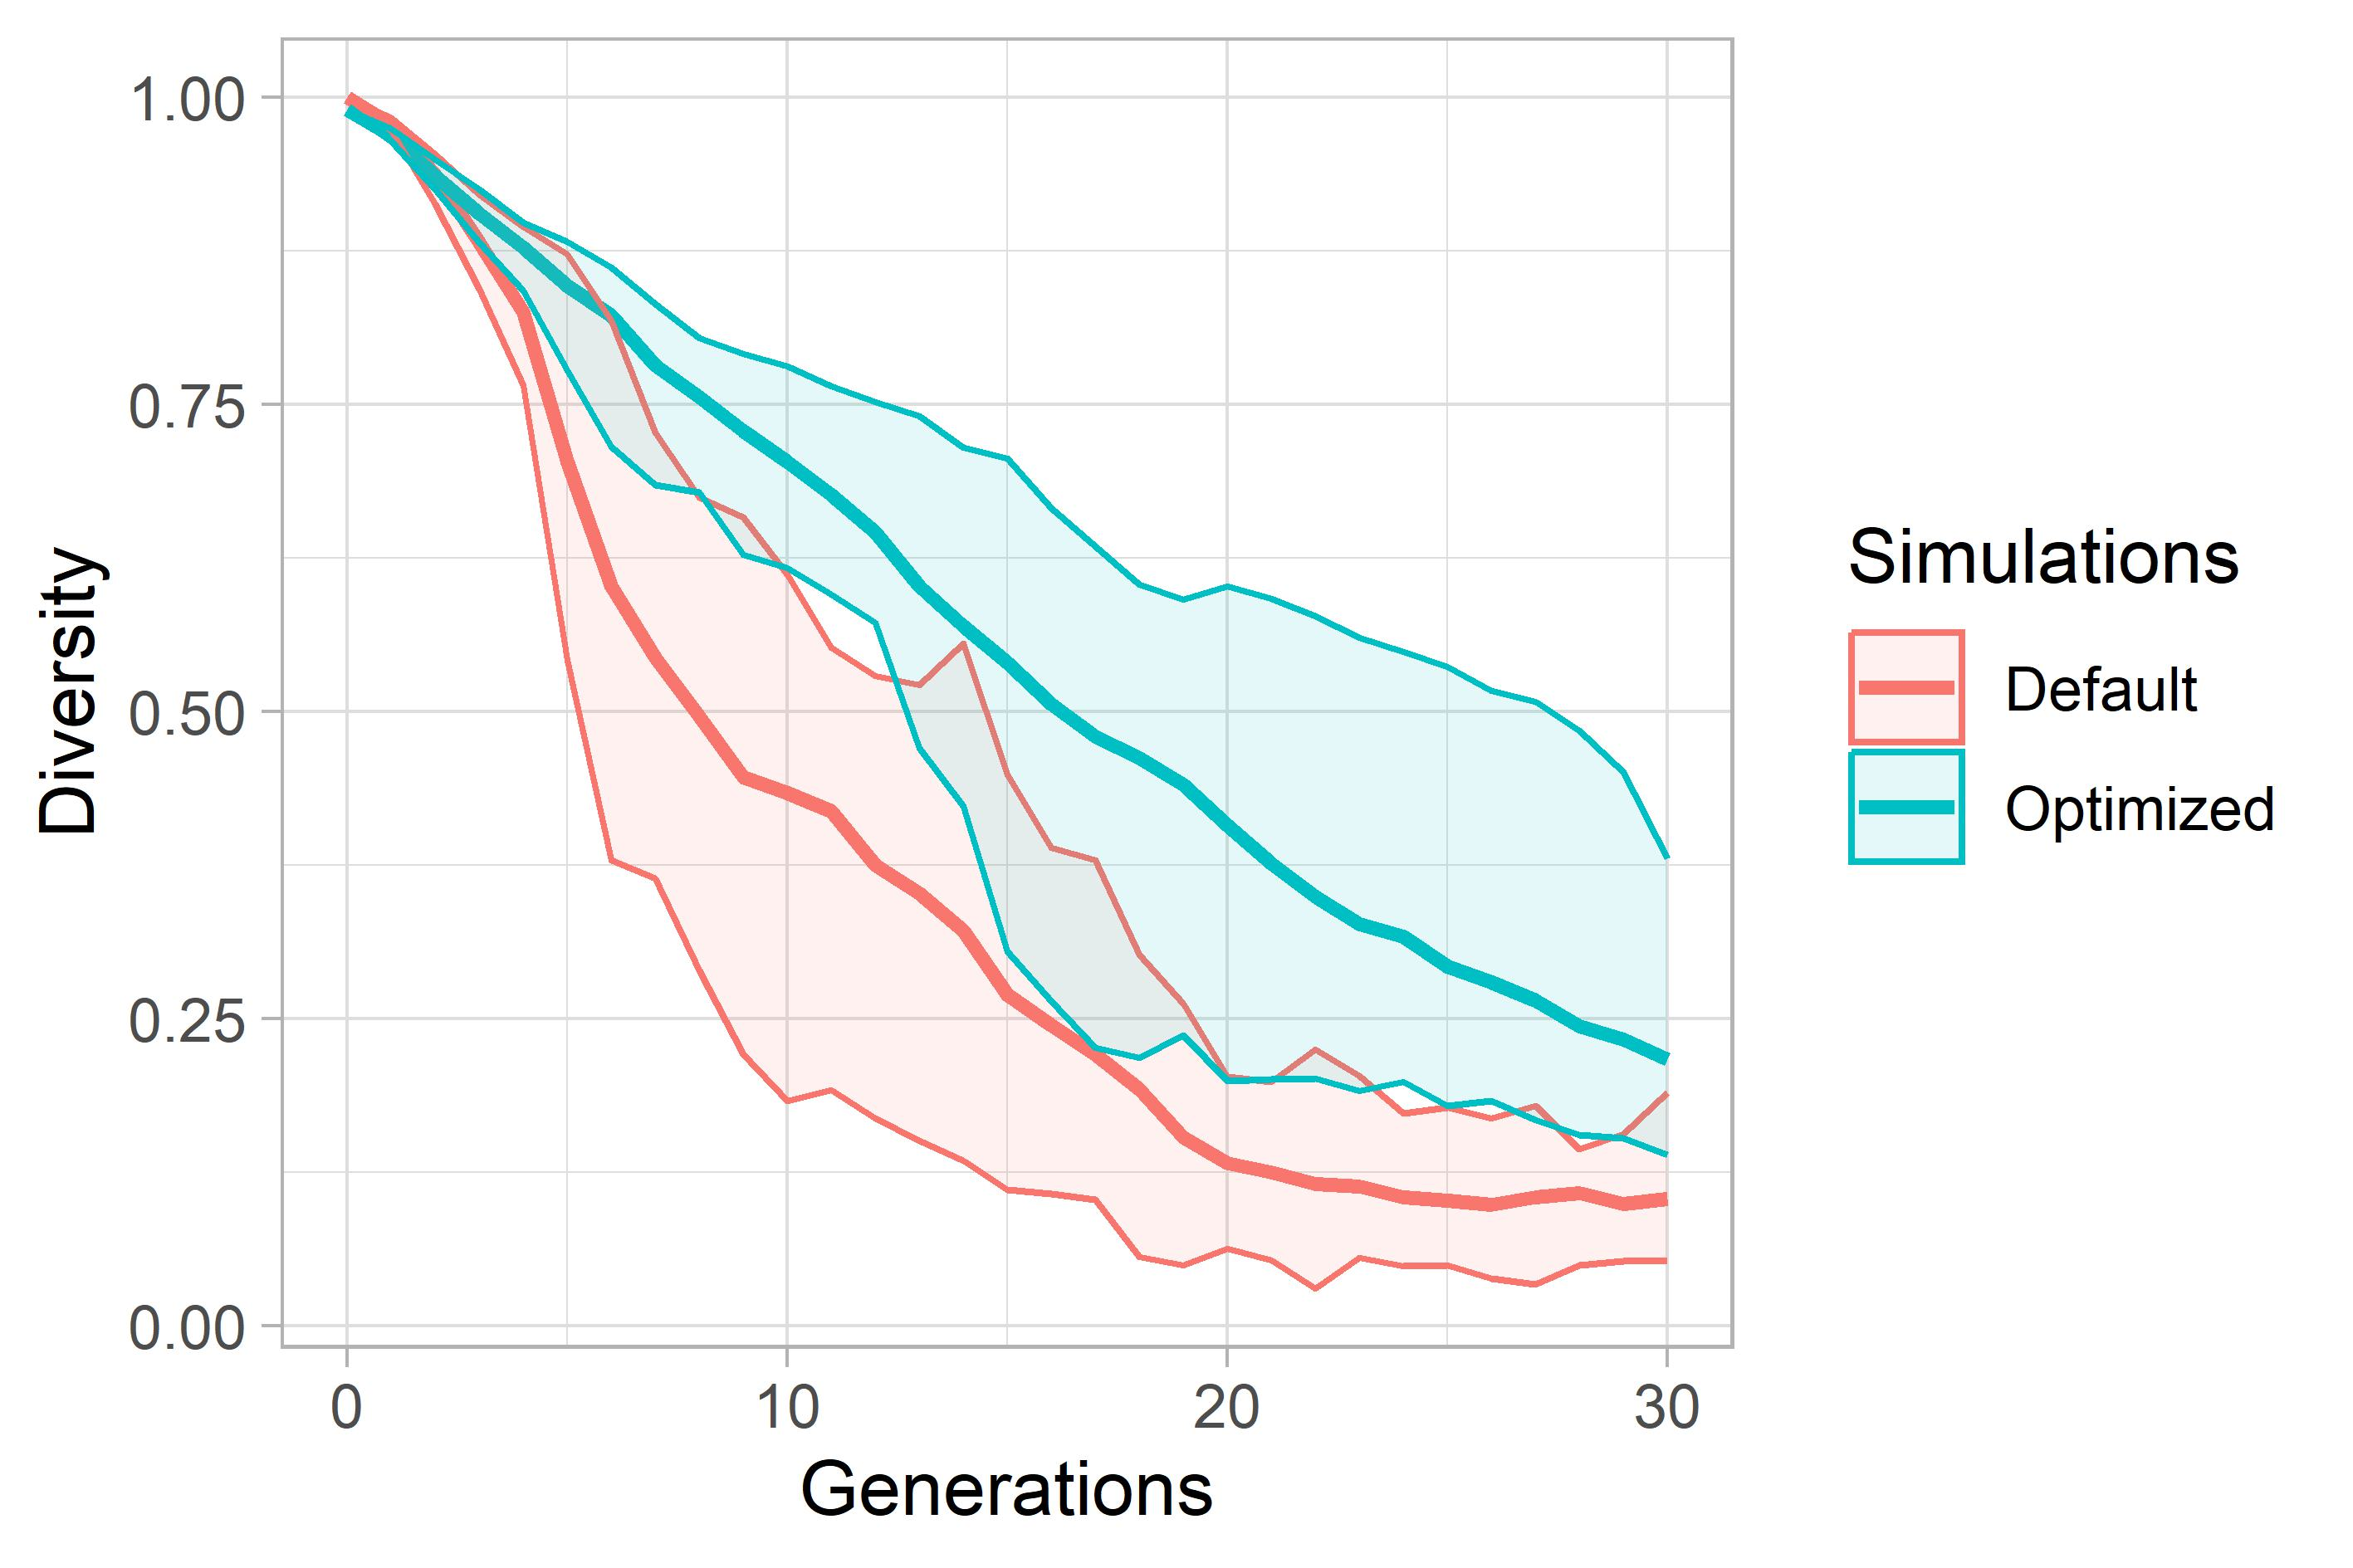
\includegraphics[width=1\linewidth]{simulations/evaluation/plots/sim_1_ga_diversity} 
	\end{minipage} 
	\caption{Start Scenario 1: Comparison of GAs}
\end{figure}

After generation 10, the rate of improved fitness of the Default GA drops compared to the Optimized GA. A combined early sharp decline in the diversity, suggests a connection. The Optimized GA shows to hold the diversity in the population longer, its rate of convergence is linear. Its high crossover and mutation rates seem to help with the improved diversity. The graph also shows, that a higher number of generations might not be useful for improved performance, as after 30 generations, the Optimized GA does not seem to hold enough diversity to continue with adequate performance gains. 

\section{Start Scenario 2}
Start scenario 2 has with 9 vehicles and 5 predestrians the same amount of NPCs as start scenario 1 and is described in more detail in Appendix \ref{fig:appendix:start_scenarios_1_2}.

\begin{figure}[ht] 
	\label{fig:evaluation:sim_2_comparison}
	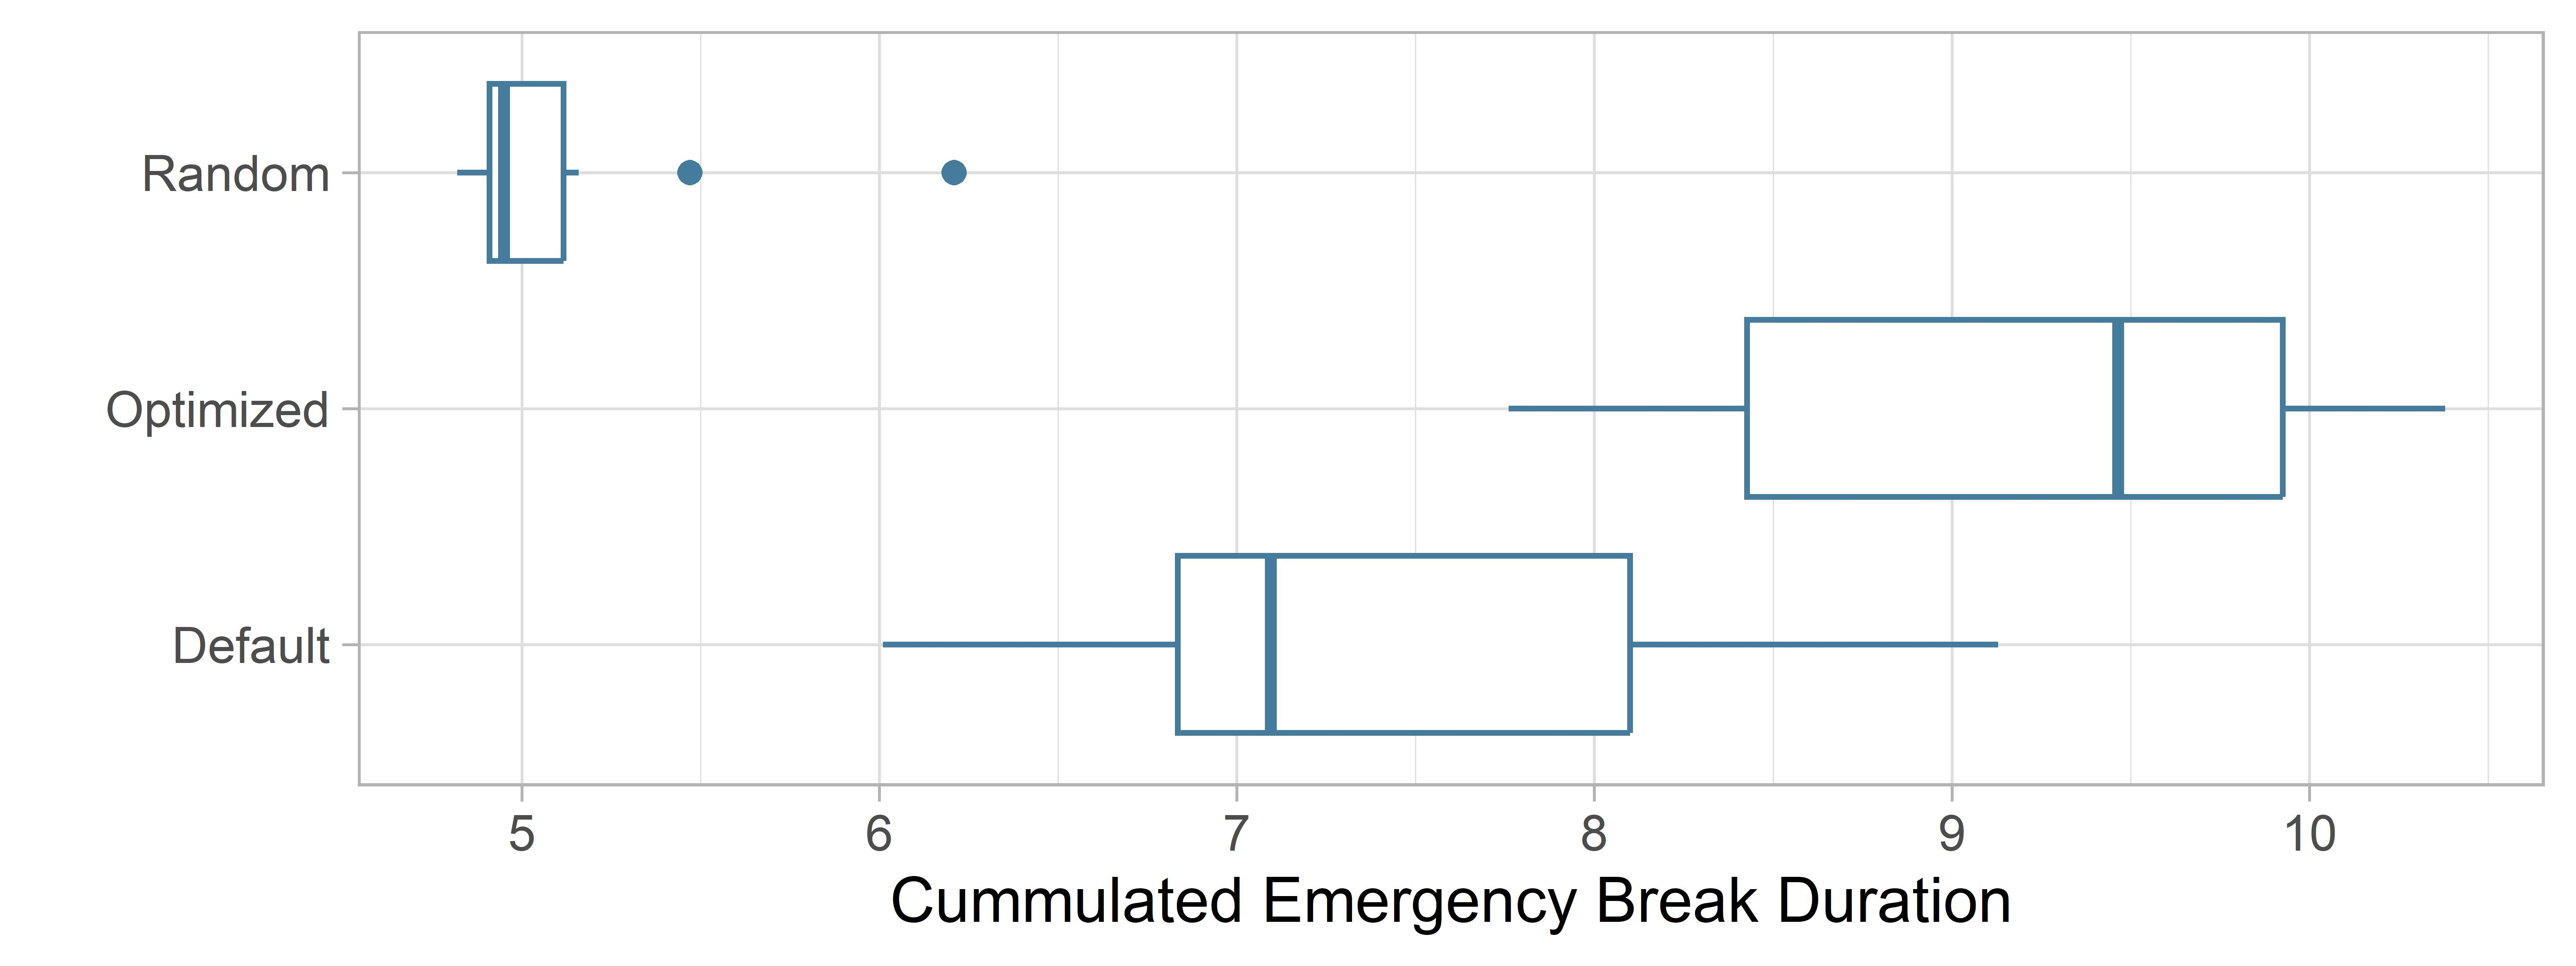
\includegraphics[width=1\linewidth]{simulations/evaluation/plots/sim_2_comparison}
	\caption{Start Scenario 2: Default GA vs Optimized GA vs Random Search}
\end{figure}

Figure \ref{fig:evaluation:sim_2_comparison} shows, that the Optimized GA can also provide better results compared to the other two algorithms in start scenarios where it has not be trained on. The Optimized GA (M = 9.24, SE = 0.3) achieves better fitness on average compared to the Default GA (M = 7.46, SE = 0.31, with a significant difference \textit{t}(17.98) = 4.19, p < 0.001 and a large effect of r = 0.7. The difference in the average fitness value compared Random Search (M = 5.13, SE = 0.13) is significant as well with \textit{t}(12.57) = 12.7, p < 0.001 and a large effect of r = 0.96.

\begin{figure}[ht] 
	\label{fig:evaluation:sim_2_ga_comparison}
	\begin{minipage}[b]{0.5\linewidth}
		\centering
		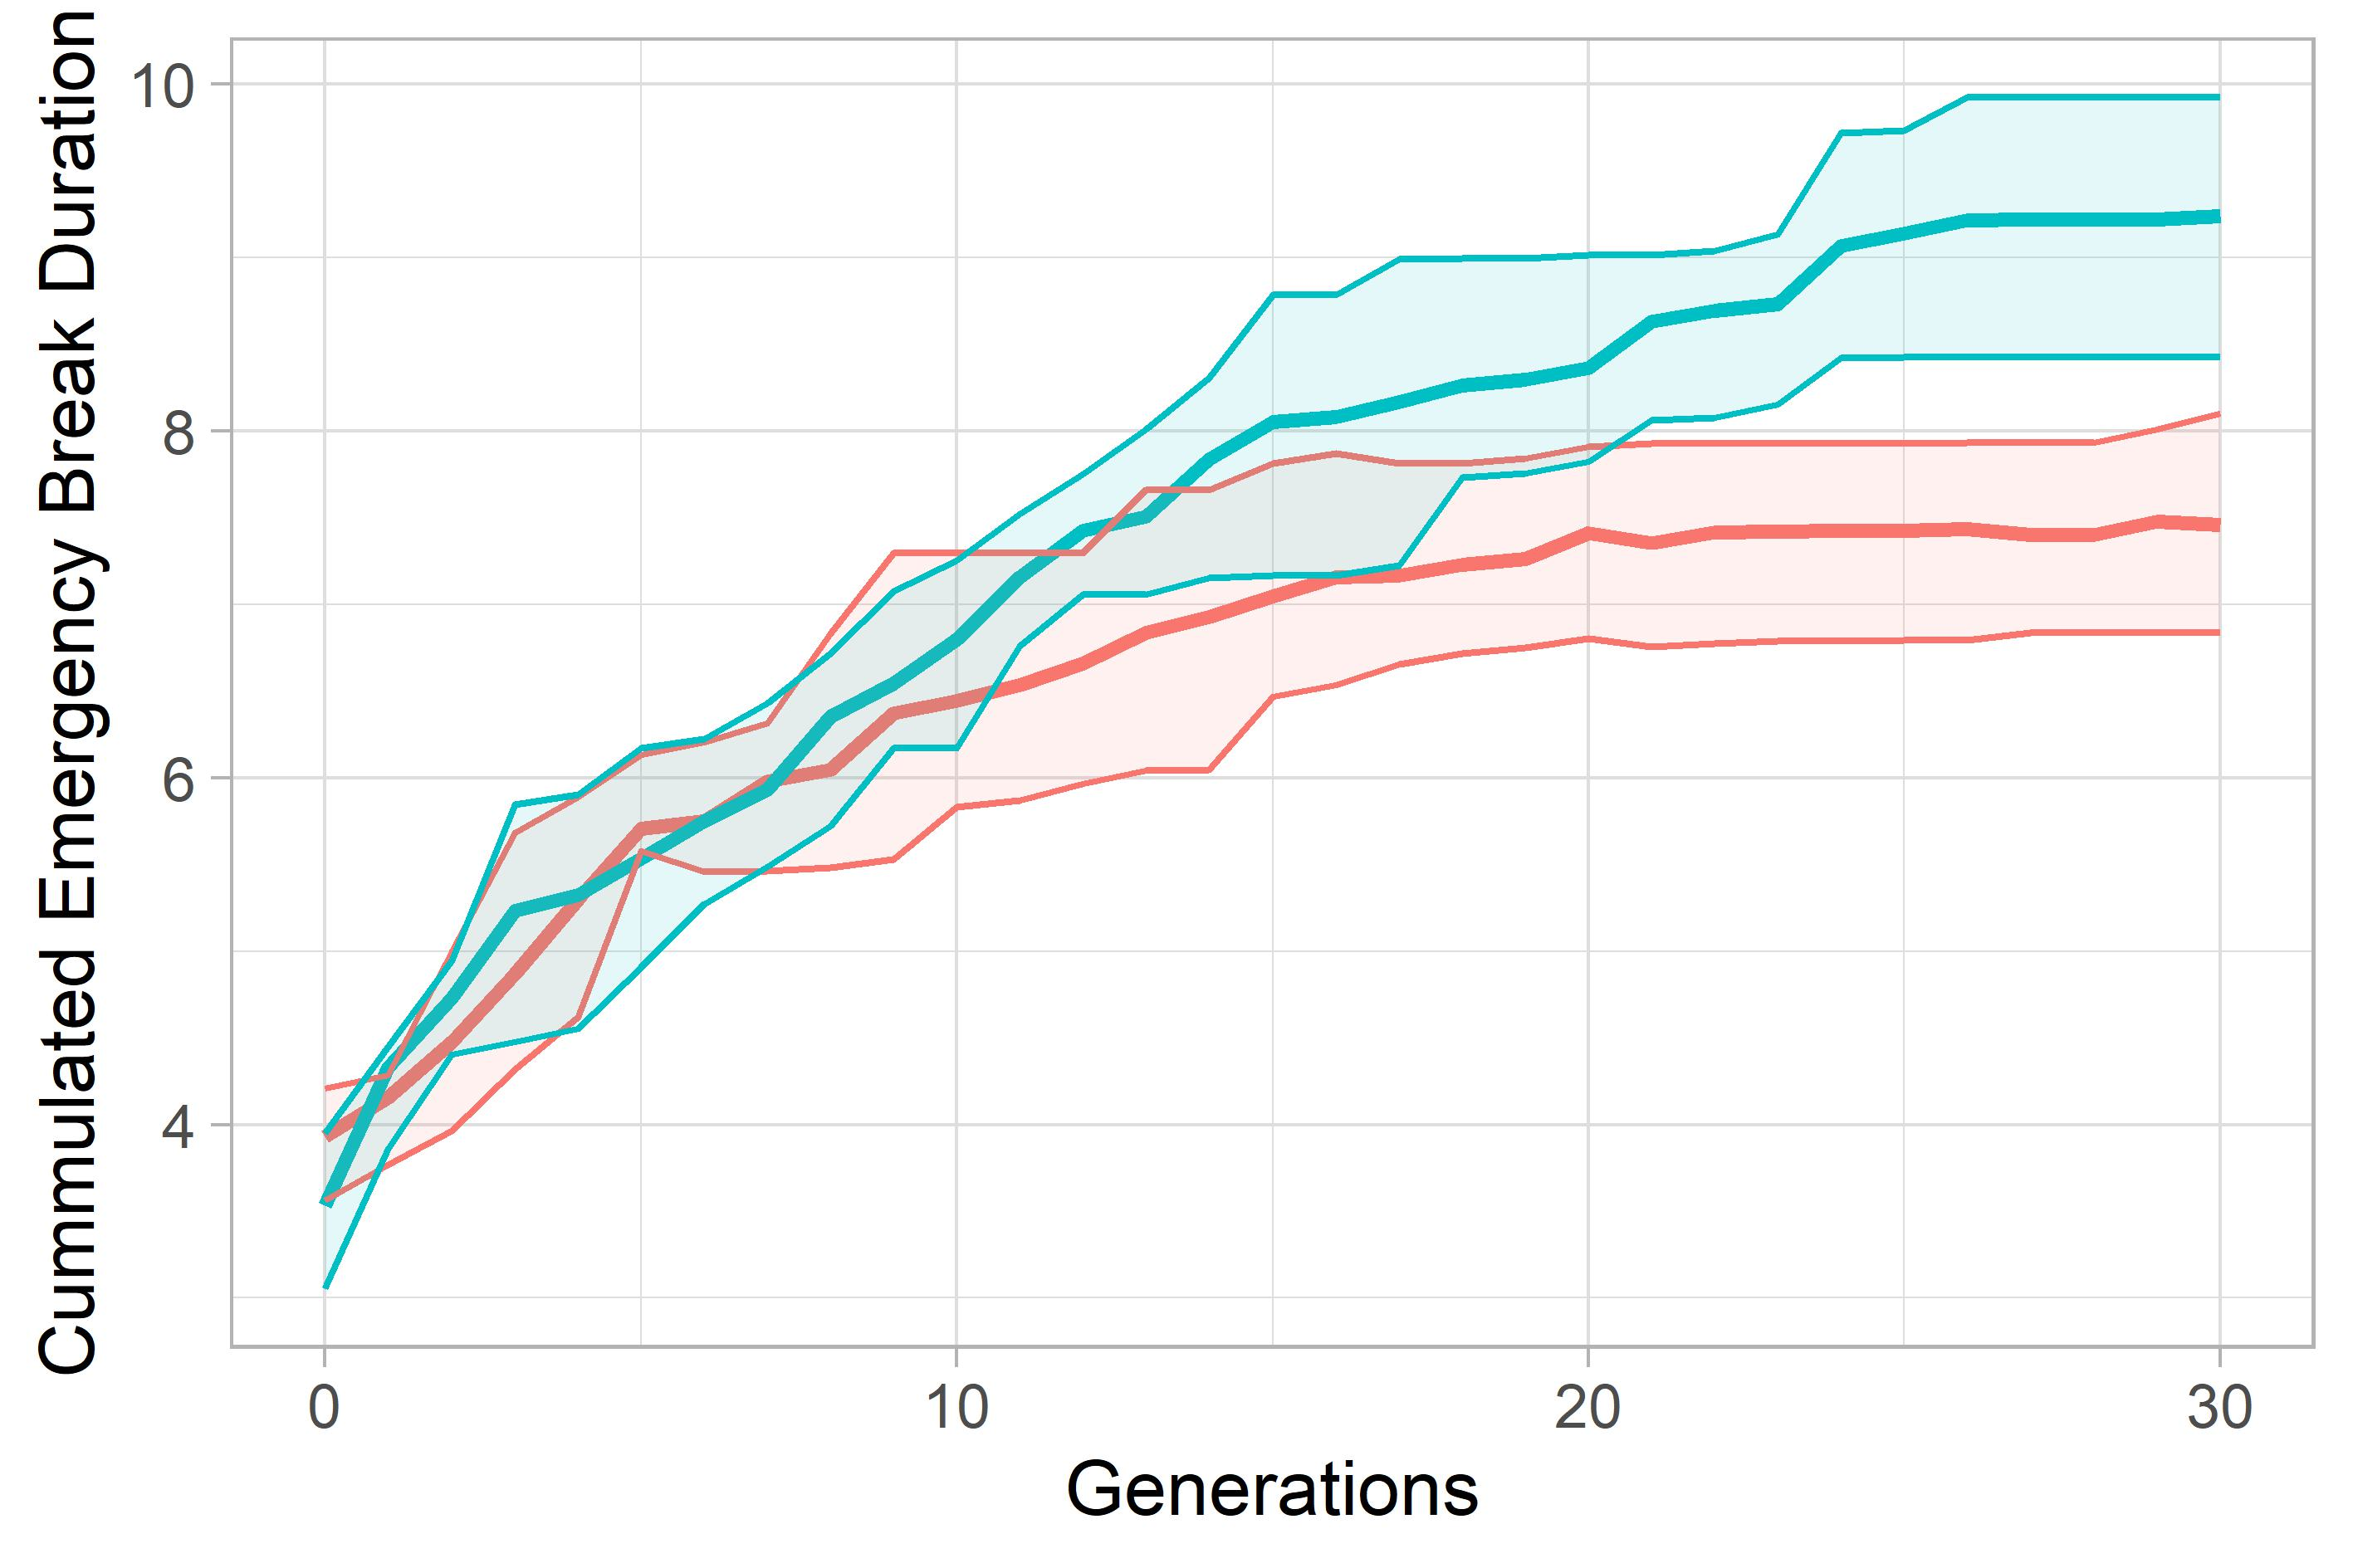
\includegraphics[width=1\linewidth]{simulations/evaluation/plots/sim_2_ga_generations} 
	\end{minipage}%%
	\begin{minipage}[b]{0.5\linewidth}
		\centering
		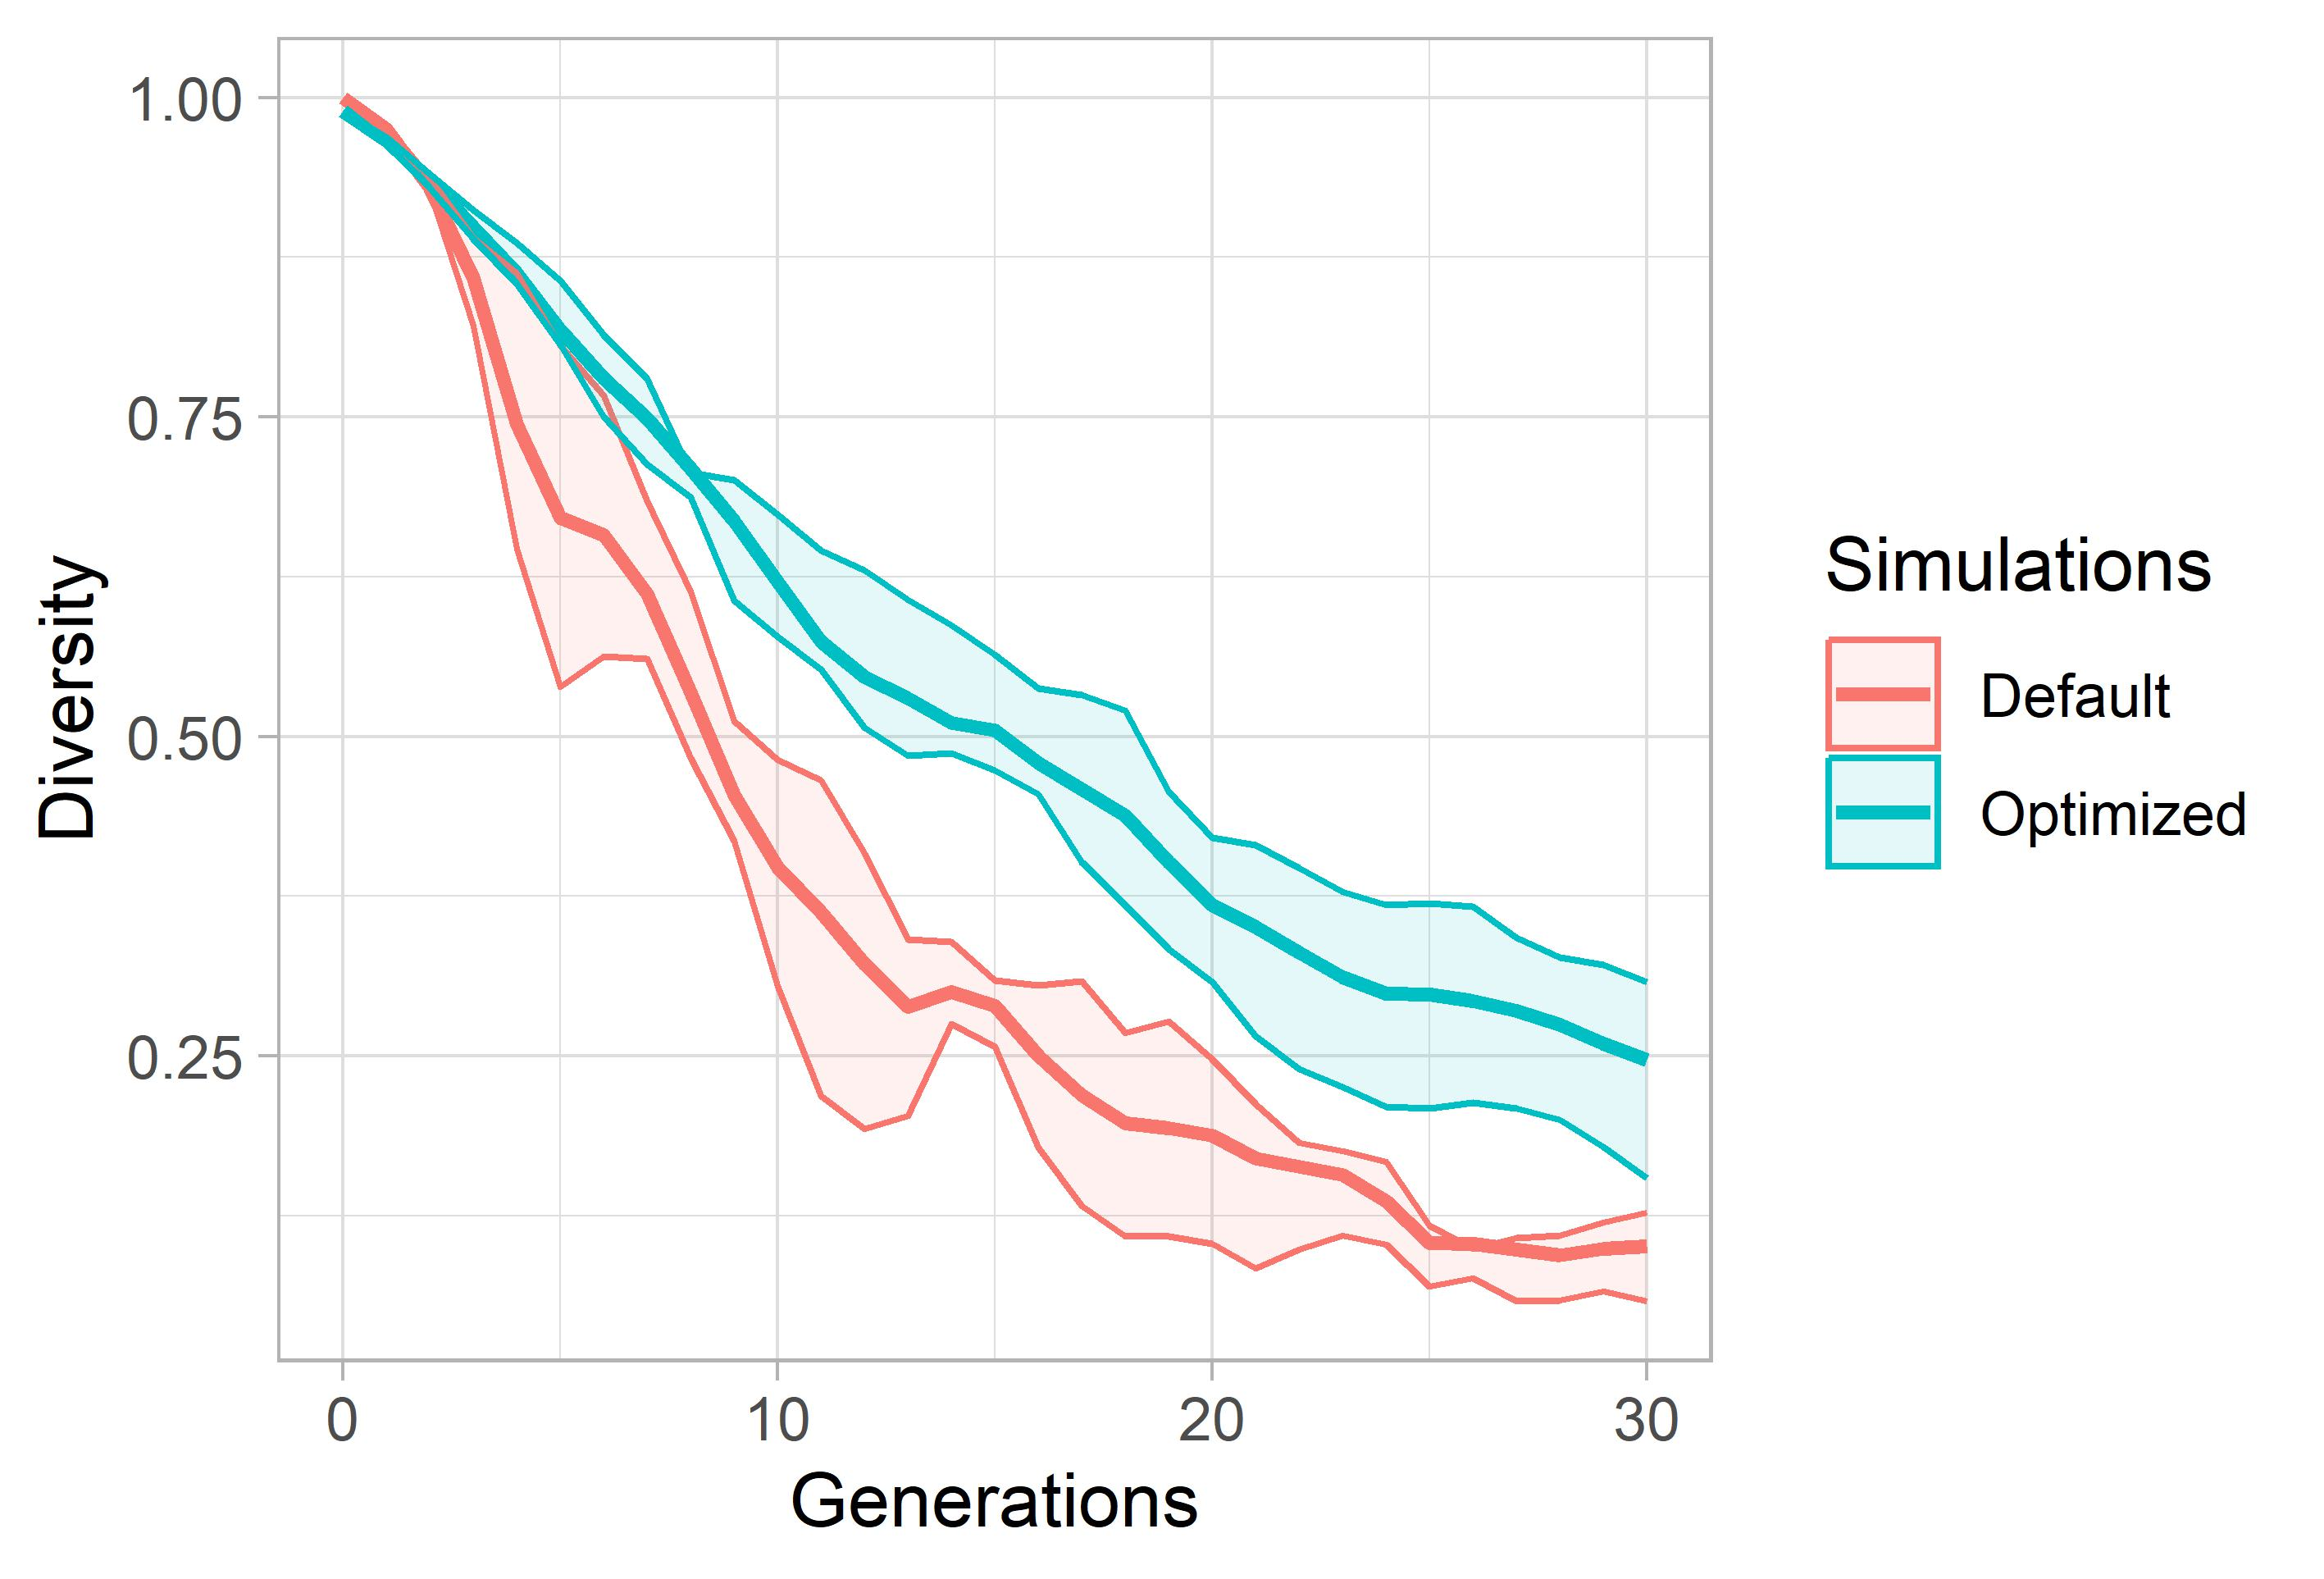
\includegraphics[width=1\linewidth]{simulations/evaluation/plots/sim_2_ga_diversity} 
	\end{minipage} 
	\caption{Start Scenario 2: Comparison of GAs}
\end{figure}

The comparison shown in Figure \ref{fig:evaluation:sim_2_ga_comparison} seams very similar to the comparison discussed in start scenario 1. On the one hand, the Default GA shows a slower performance increase starting already from generation 8. On the other hand, the diversity of the Optimized GA drops a bit sooner. Still both evaluations show, that the Optimized GA performs well in start scenarios with the given amount of NPCs.

\section{Start Scenario 3}
\label{sect:evaluation:scenario_3}
Start scenario 3 is described in more detail in Appendix \ref{fig:appendix:start_scenarios_3_4}. 5 vehicles with 3 pedestrians are initialized, resulting in a simulation with only a small number of NPCs.

\begin{figure}[ht] 
	\label{fig:evaluation:sim_3_comparison}
	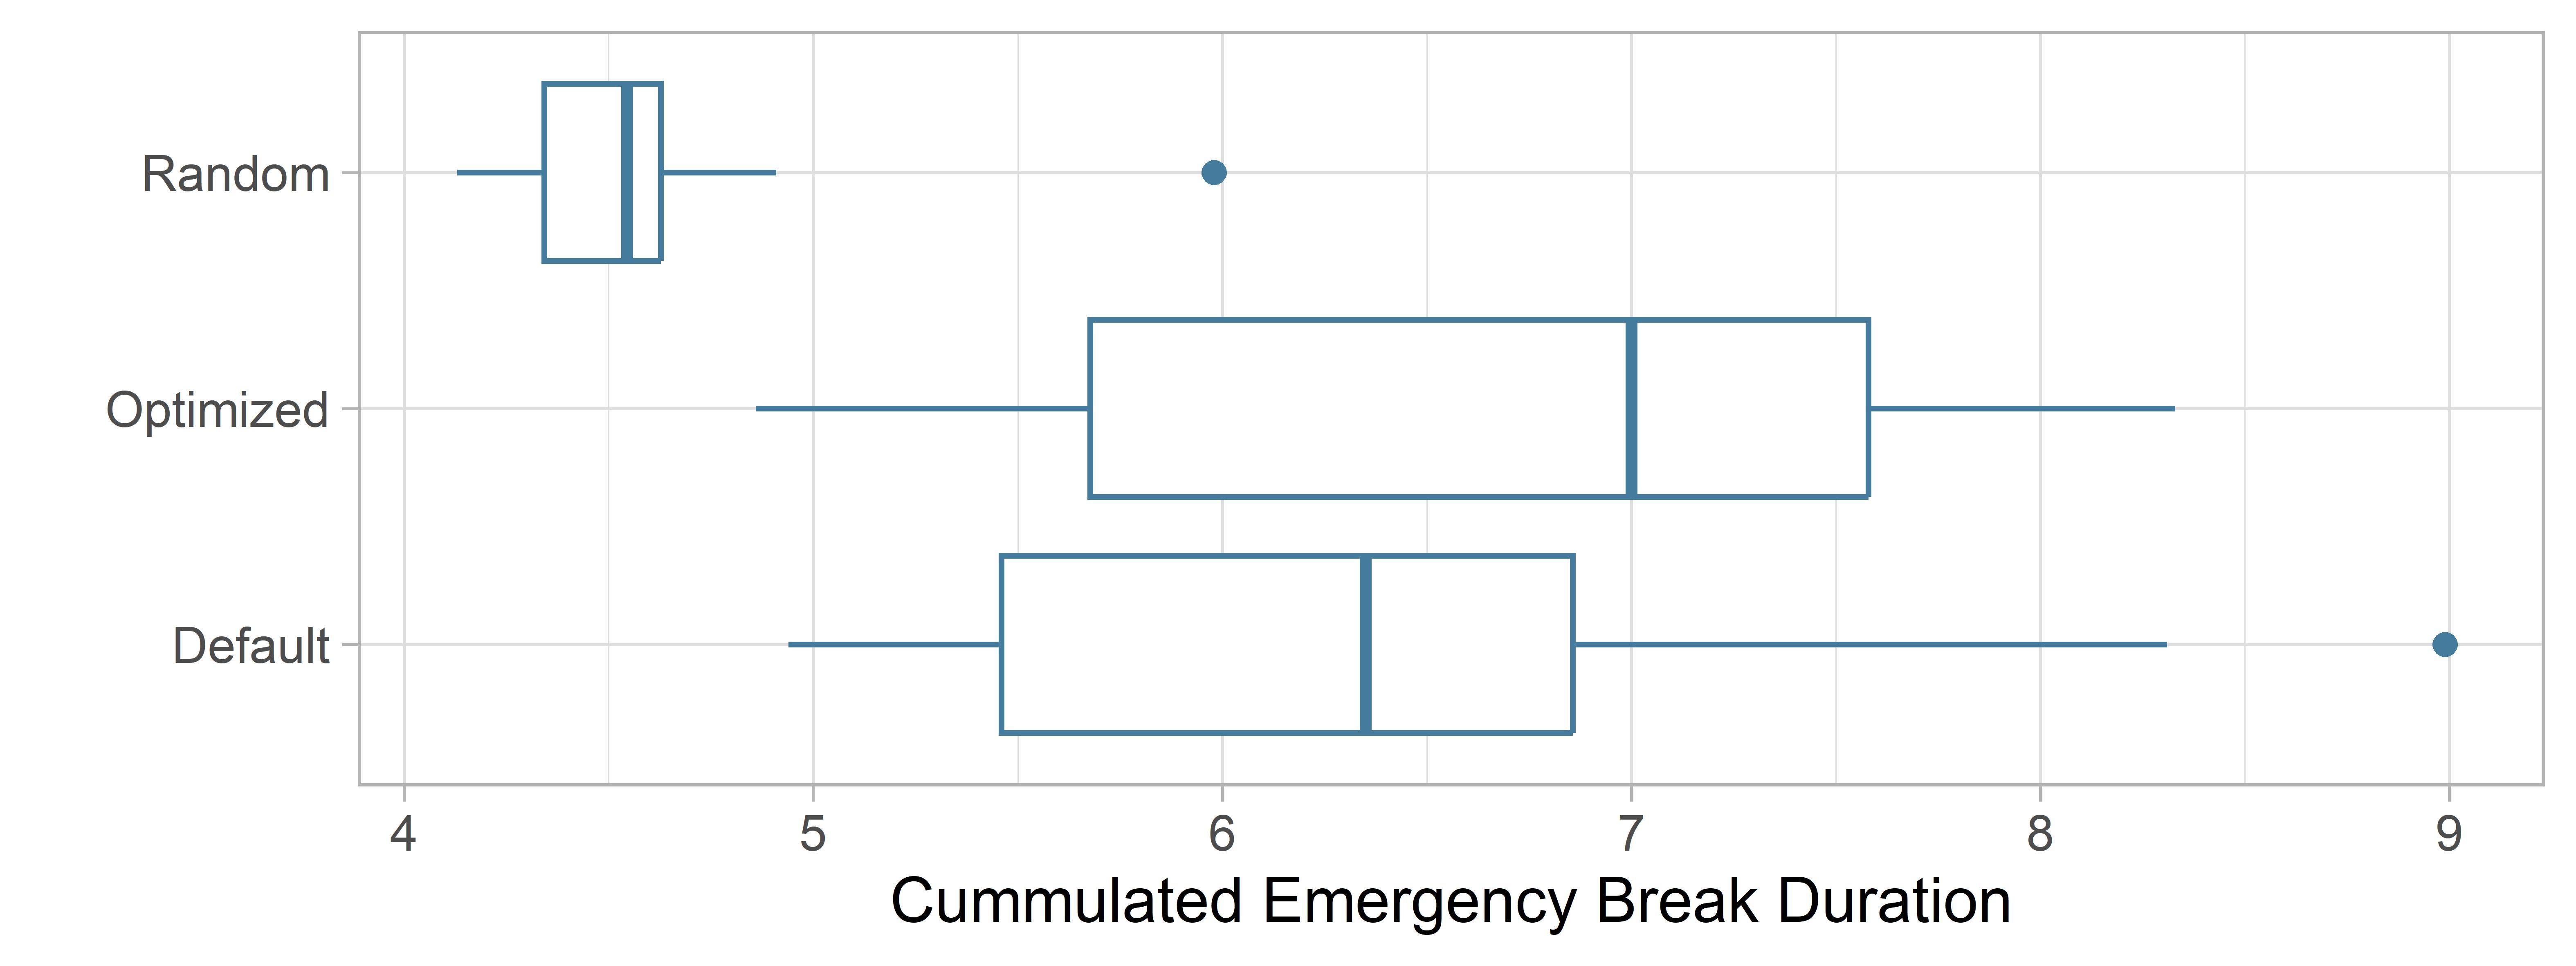
\includegraphics[width=1\linewidth]{simulations/evaluation/plots/sim_3_comparison}
	\caption{Start Scenario 3: Default GA vs Optimized GA vs Random Search}
\end{figure}

Looking at the graph, the Optimized GA again outperforms the Random Search, however there seams to be only marginal improvements compared to Default GA.  A t-test confirms these findings. While on average, greater fitness is achieved by using Optimized GA (M = 6.66, SE = 0.38) than from using Default GA (M = 6.49, SE = 0.42). This difference was however not significant \textit{t}(17.83) = 0.29, p > .05 and an effect size of r = 0.07.
Verifying the better performance of the Optimized GA compared to Random Search (M = 4.619, SE = 0.17) shows a significant difference \textit{t}(12.4) = 4.9, p < .001 and a large effect size of r = 0.81.

To further analyse both genetic algorithms, their performance over the generations next to their diversity chart is again shown in Figure \ref{fig:evaluation:sim_3_ga_comparison}. The mean over 10 repetitions is plotted, the outline show the first and third quantiles.

\begin{figure}[ht] 
	\label{fig:evaluation:sim_3_ga_comparison}
	\begin{minipage}[b]{0.5\linewidth}
		\centering
		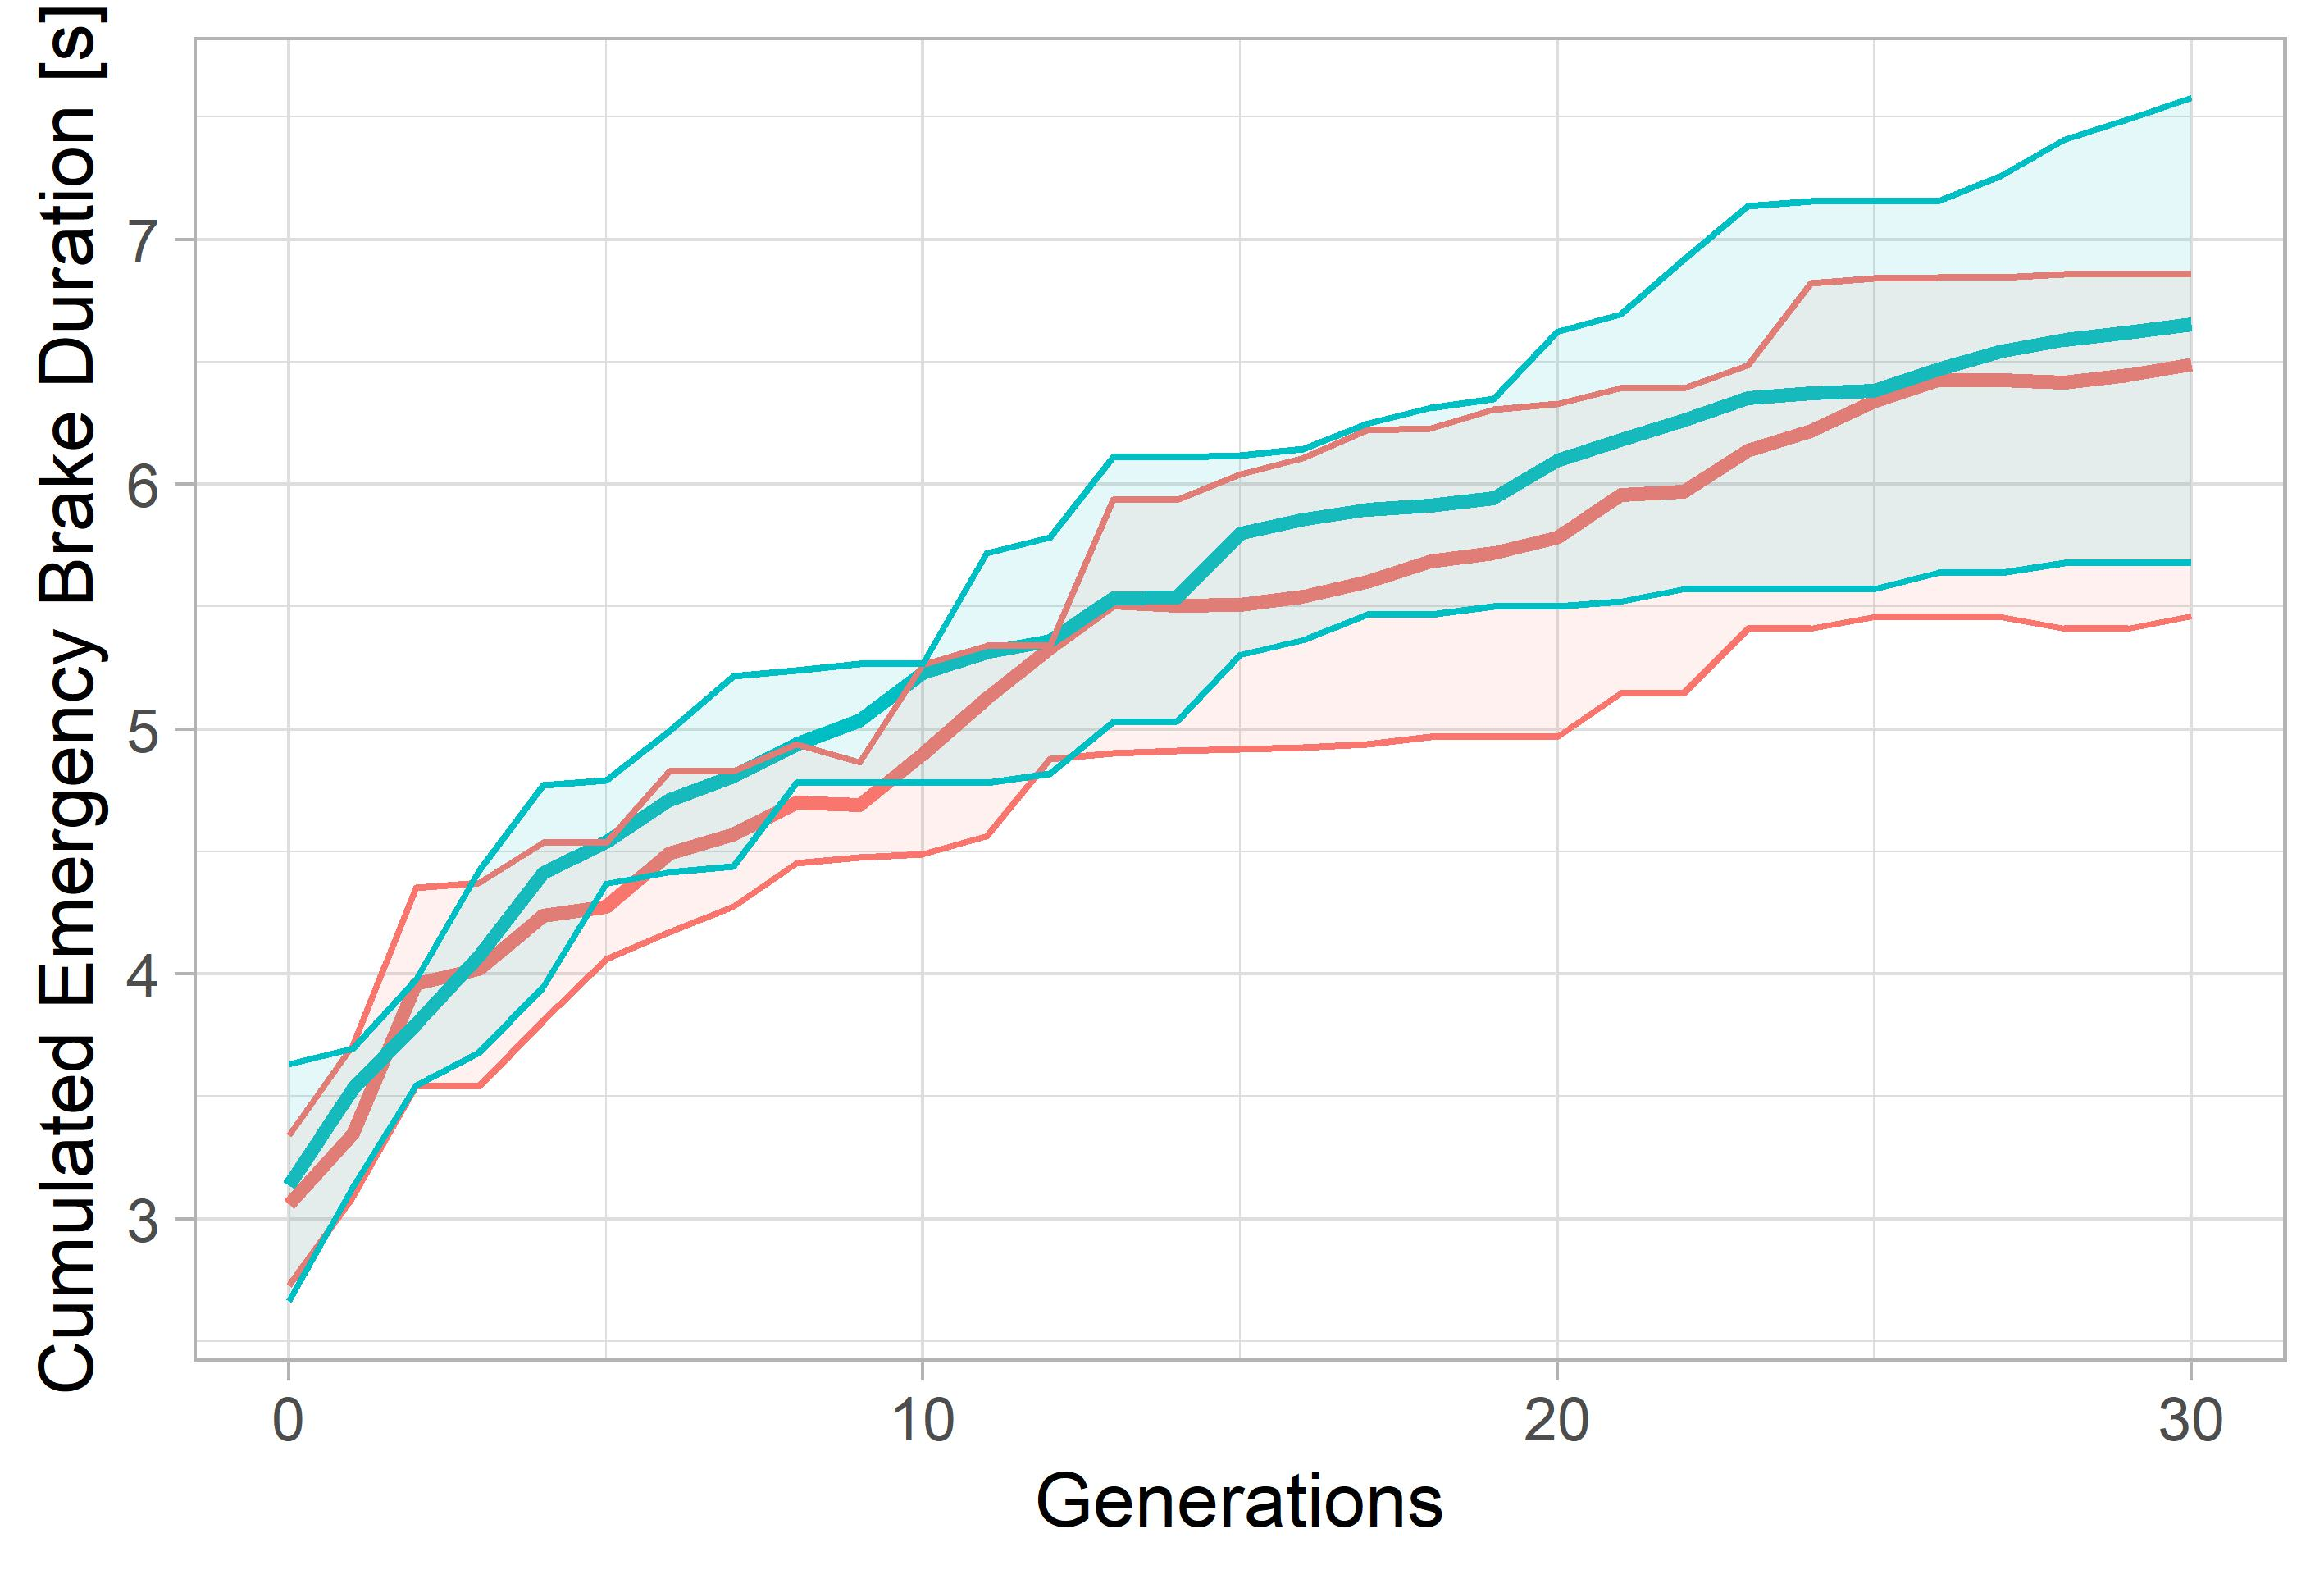
\includegraphics[width=1\linewidth]{simulations/evaluation/plots/sim_3_ga_generations} 
	\end{minipage}%%
	\begin{minipage}[b]{0.5\linewidth}
		\centering
		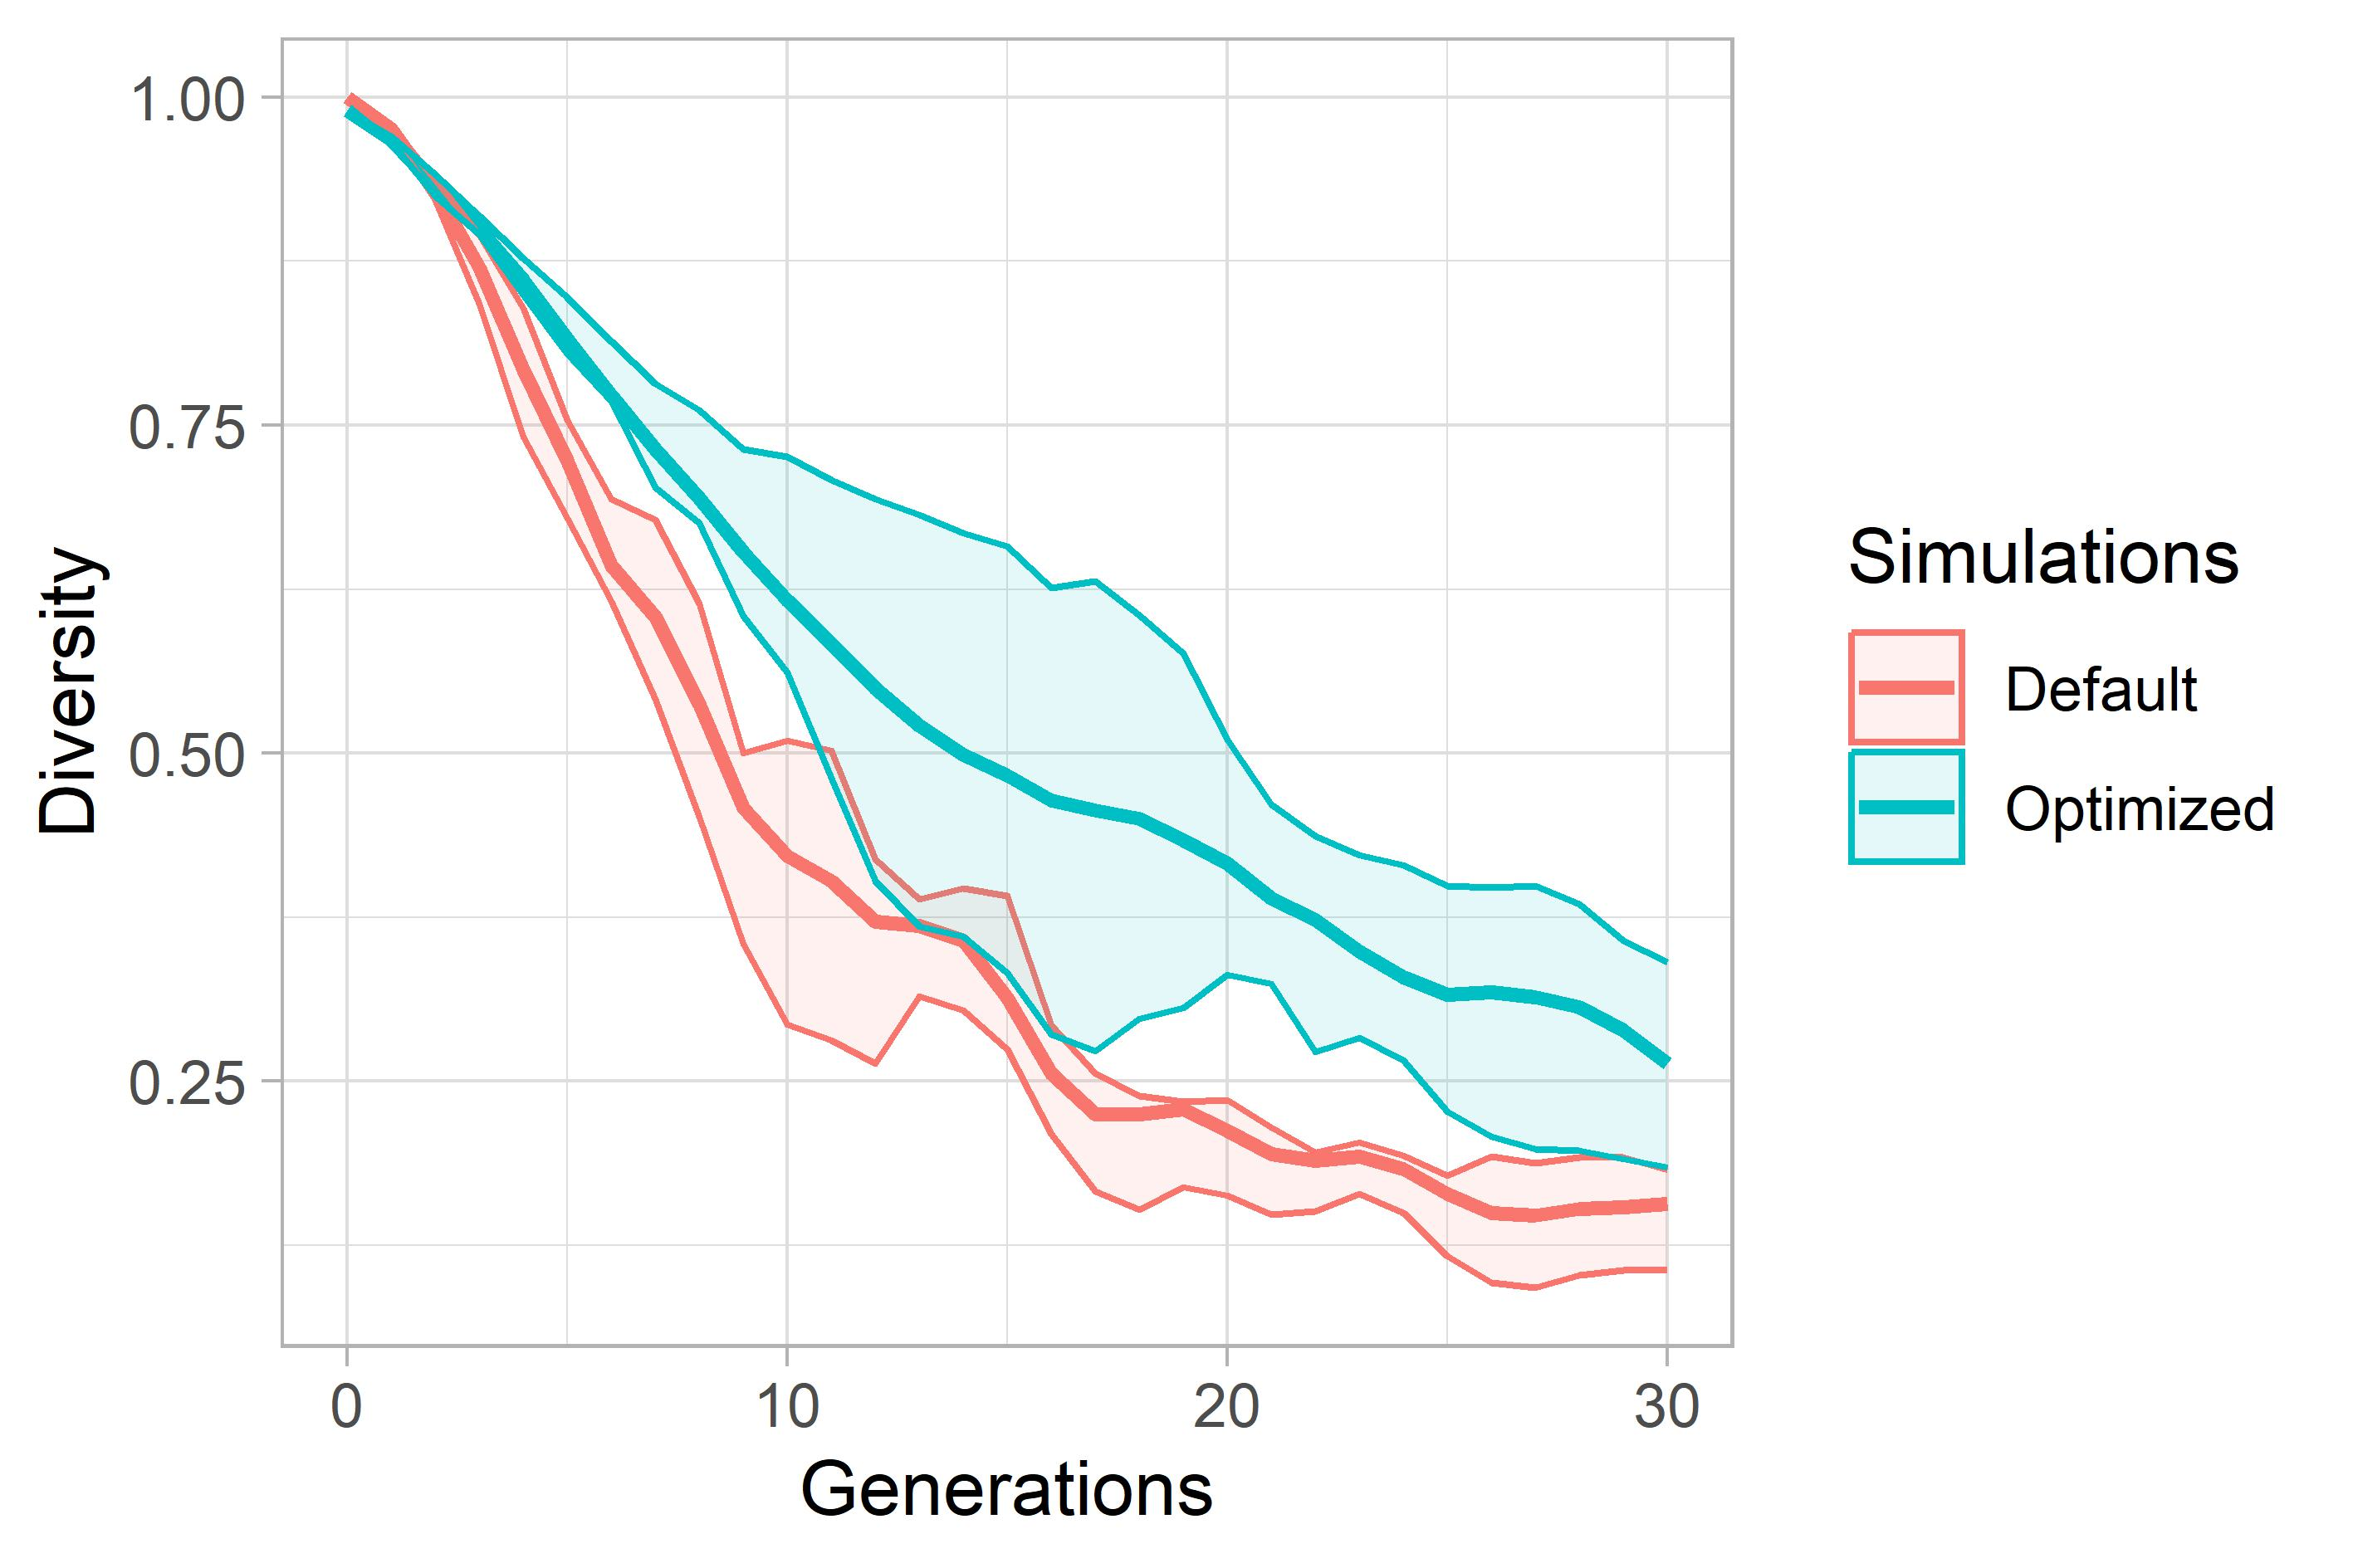
\includegraphics[width=1\linewidth]{simulations/evaluation/plots/sim_3_ga_diversity} 
	\end{minipage} 
	\caption{Start Scenario 3: Comparison of GAs}
\end{figure}


The rate of improved fitness of the Default GA now drops very similar to the Optimized GA. The early decline in the diversity is also not as pronounced as in the previous comparisons. While the optimized GA shows to still hold the diversity in the population longer, this only has a minimal impact on its average fitness. The similarity in performance might be explained by the smaller search space due to the smaller number of NPCs. Here, high mutation and crossover rates might not have the previous pronounced advantage.

\section{Start Scenario 4}
Start scenario 4 can be seen in Appendix at \ref{fig:appendix:start_scenarios_3_4}. 18 vehicles with 10 pedestrians are initialized, resulting in the simulation with the most NPCs.

\begin{figure}[ht] 
	\label{fig:evaluation:sim_4_comparison}
	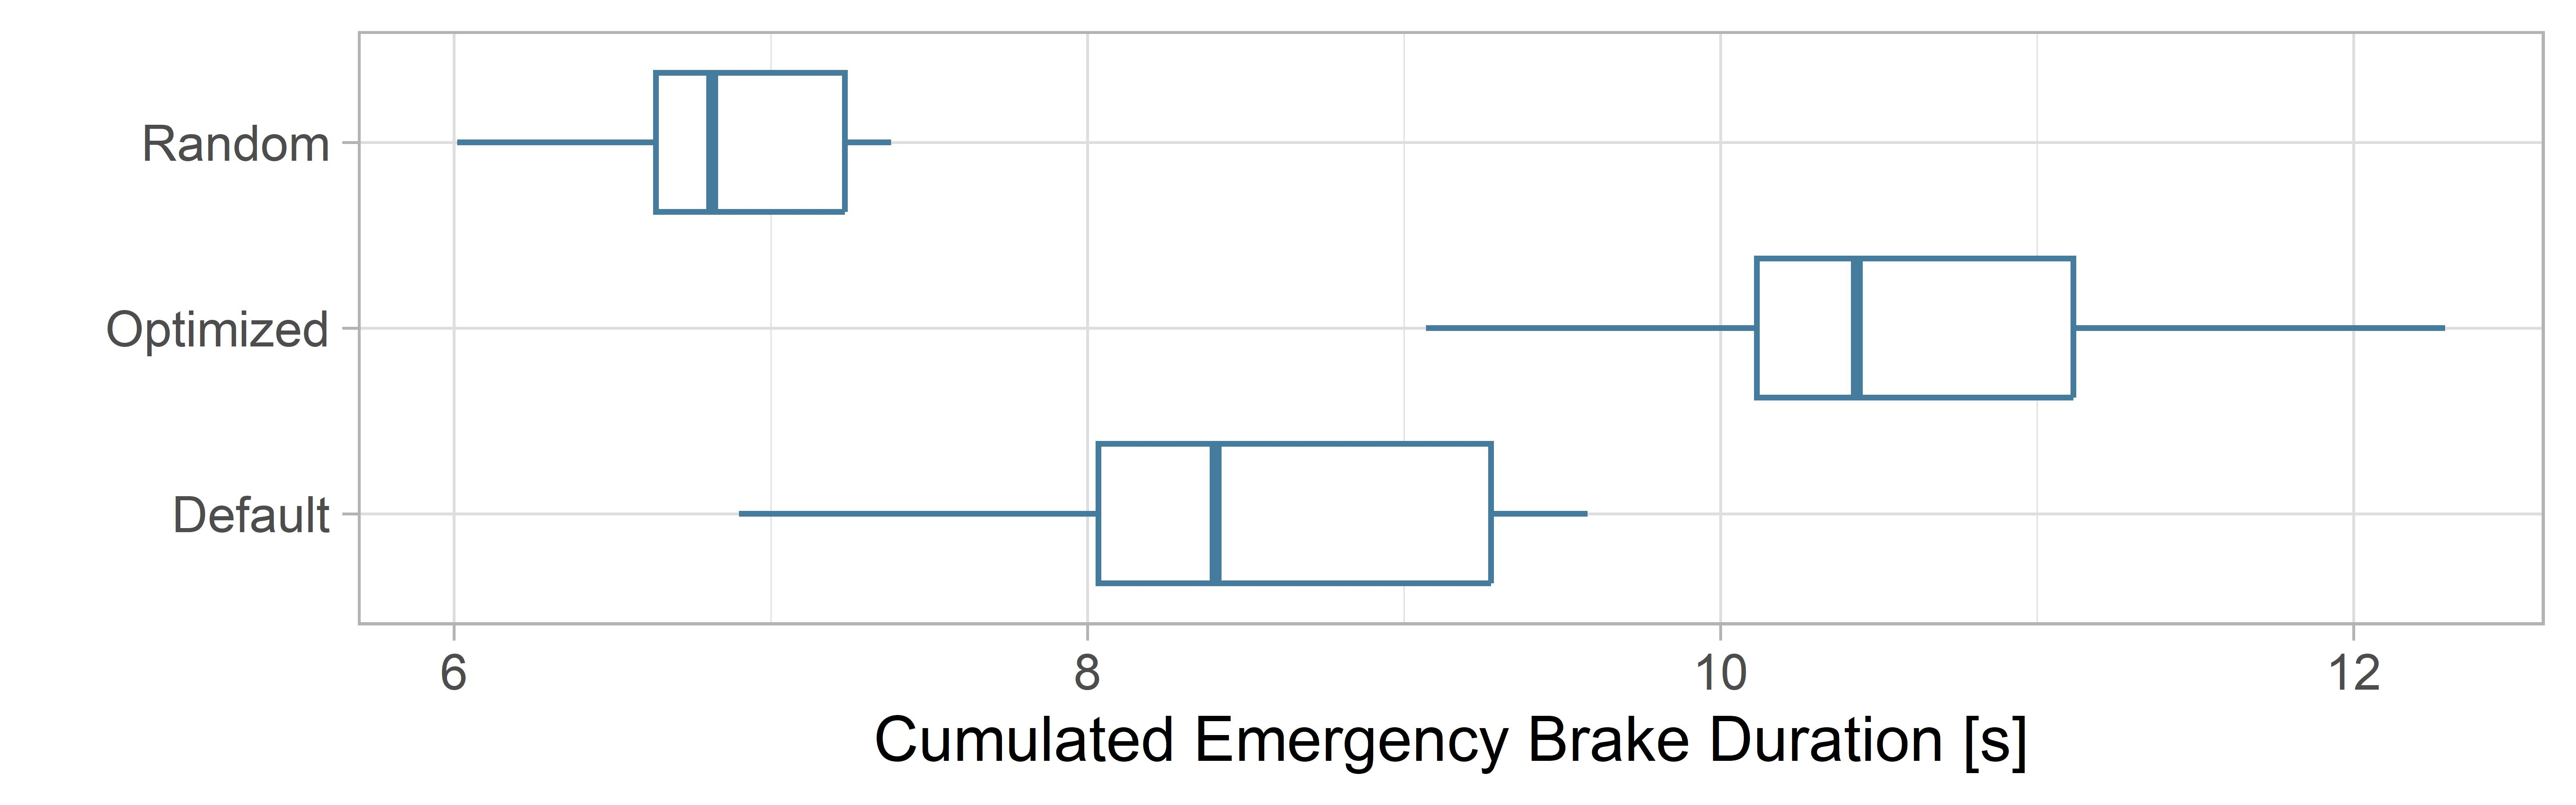
\includegraphics[width=1\linewidth]{simulations/evaluation/plots/sim_4_comparison}
	\caption{Start Scenario 4: Default GA vs Optimized GA vs Random Search}
\end{figure}

Figure \ref{fig:evaluation:sim_4_comparison} shows the Optimized GA clearly outperforming the Default GA as well as Random Search.
The Optimized GA (M = 10.60, SE = 0.29) has significantly greater fitness then the Default GA (M = 8.46, SE = 0.28) with \textit{t}(17.98) = 5.30, p < .001 and a large effect r = 0.78.
Compared to Random Search (M = 6.86, SE = 0.14), the greater fitness of the Optimized GAs is significant with \textit{t}(11.71) = 12.7, p < .001 and a large effect r = 0.96. Both genetic algorithms performance over the generations next to their diversity chart is compared in Figure \ref{fig:evaluation:sim_4_ga_comparison}.

\begin{figure}[ht] 
	\label{fig:evaluation:sim_4_ga_comparison}
	\begin{minipage}[b]{0.5\linewidth}
		\centering
		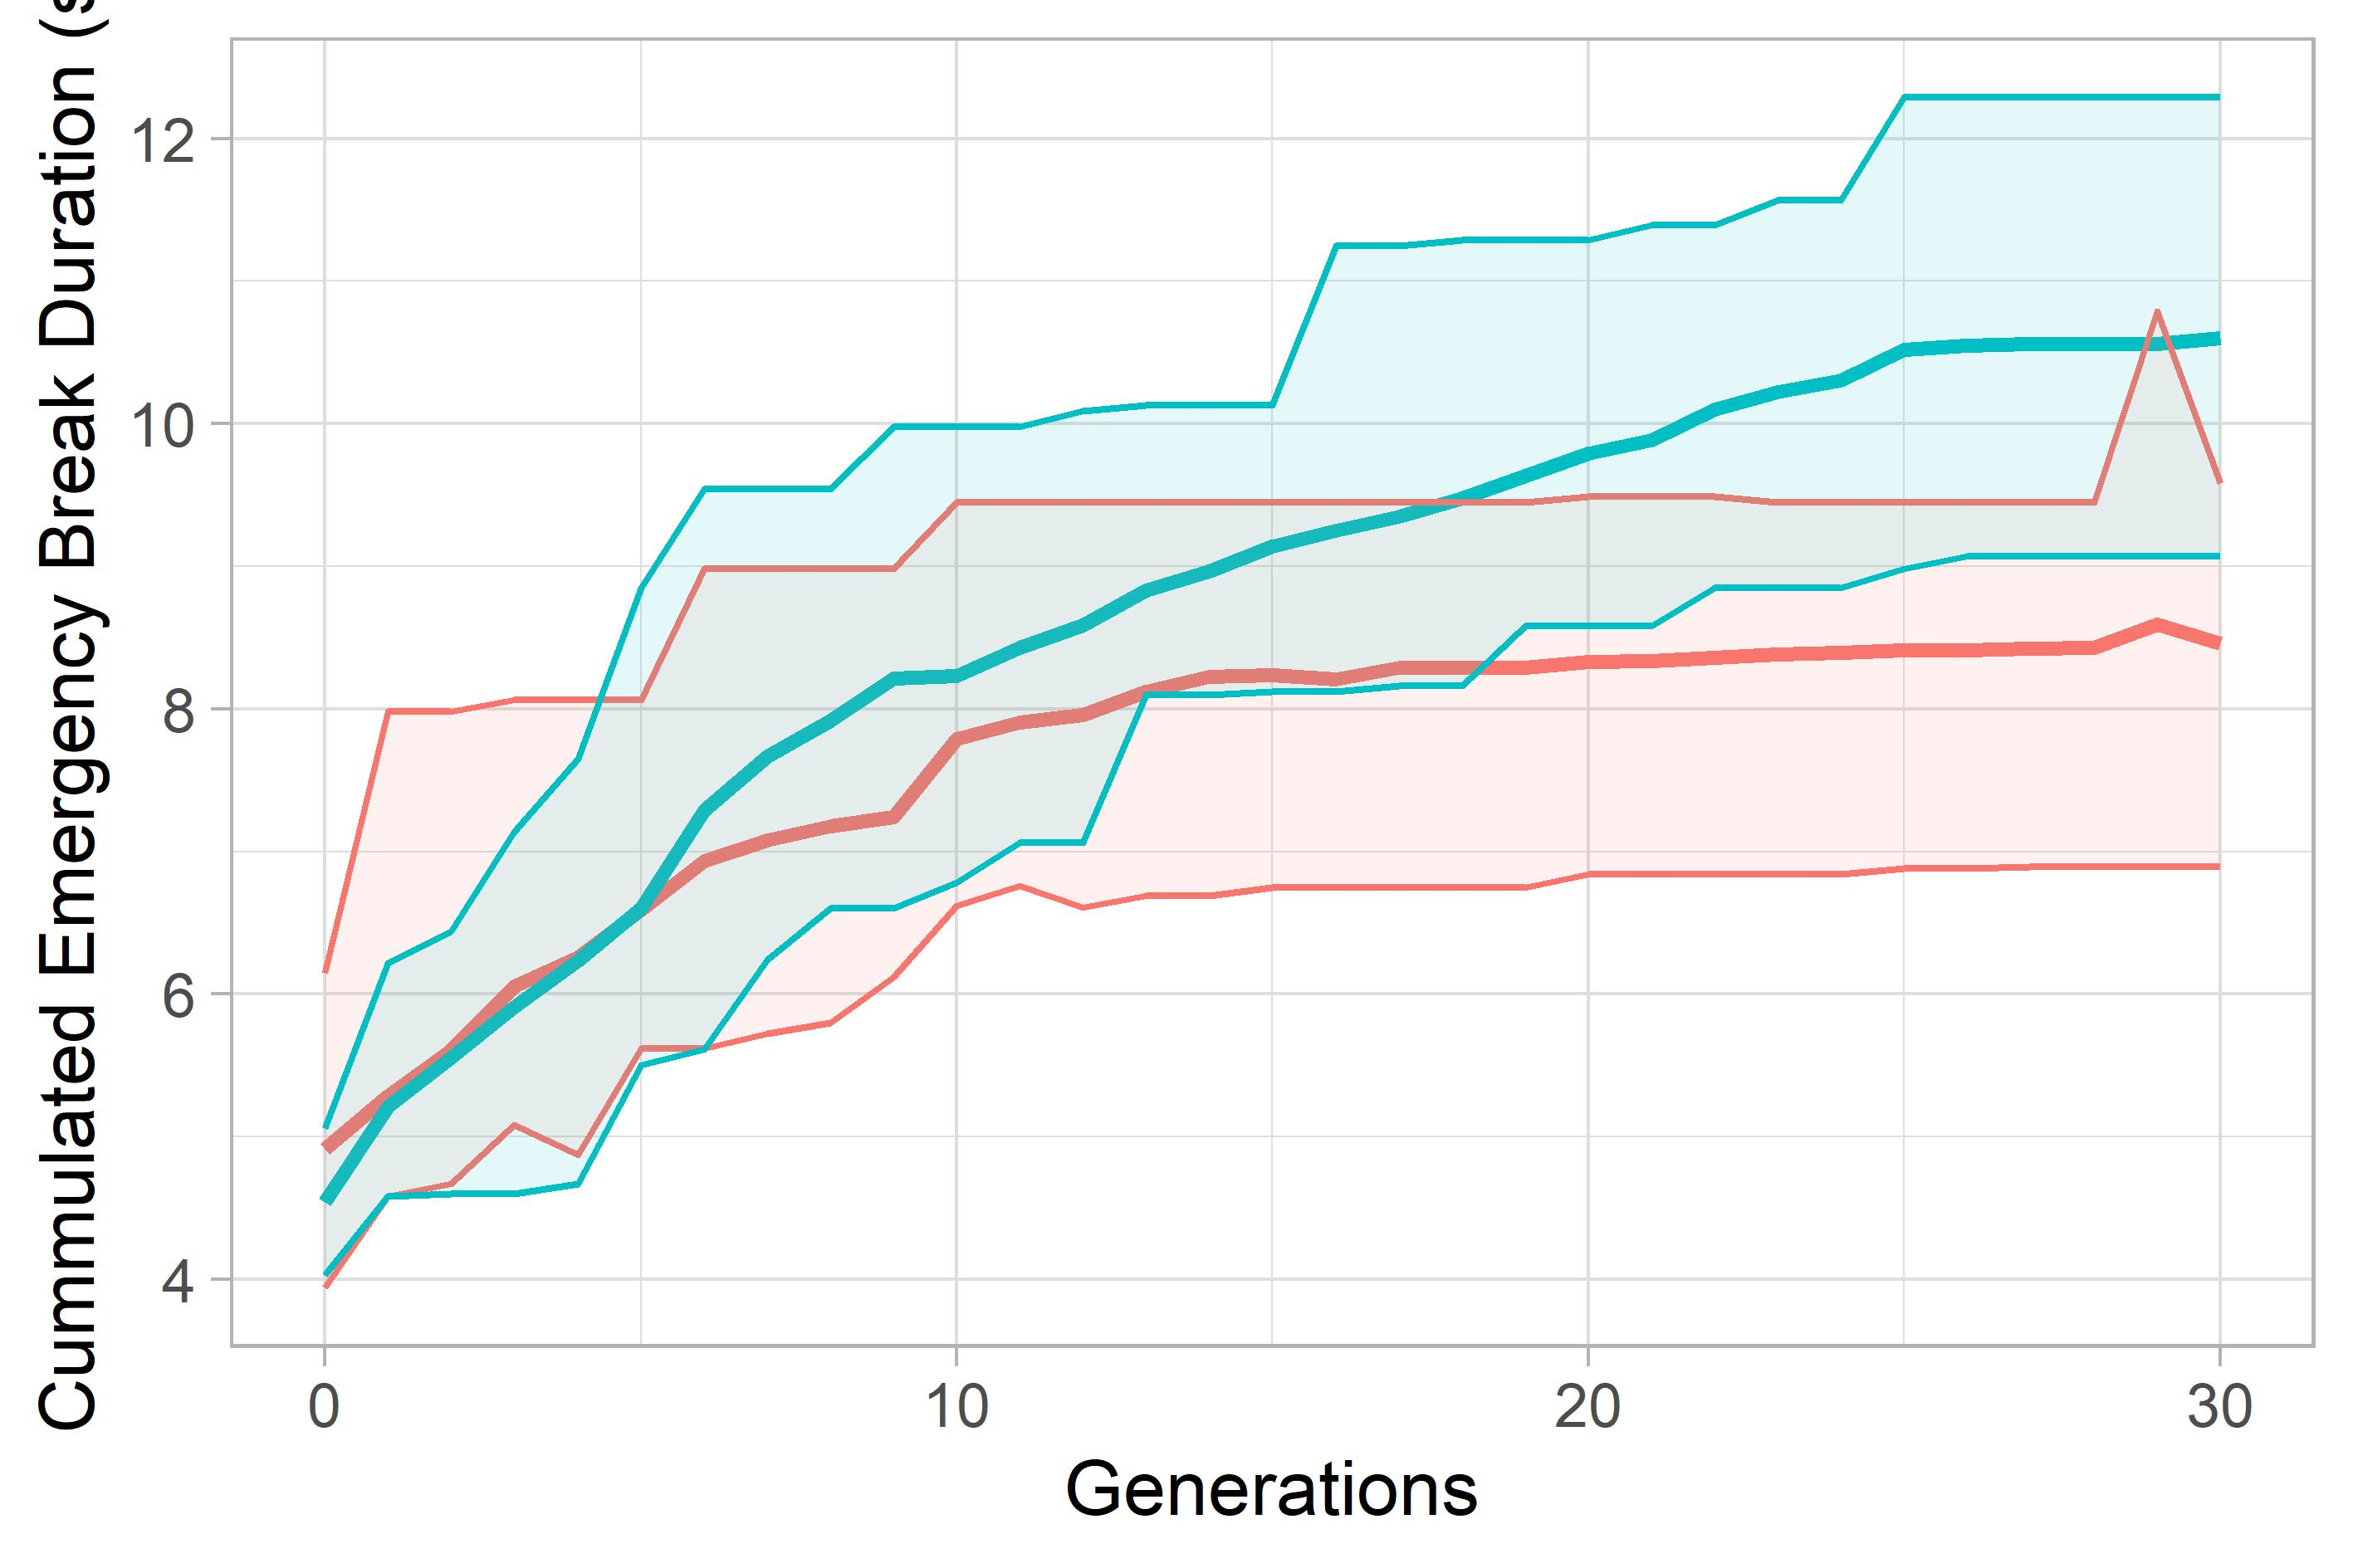
\includegraphics[width=1\linewidth]{simulations/evaluation/plots/sim_4_ga_generations} 
	\end{minipage}%%
	\begin{minipage}[b]{0.5\linewidth}
		\centering
		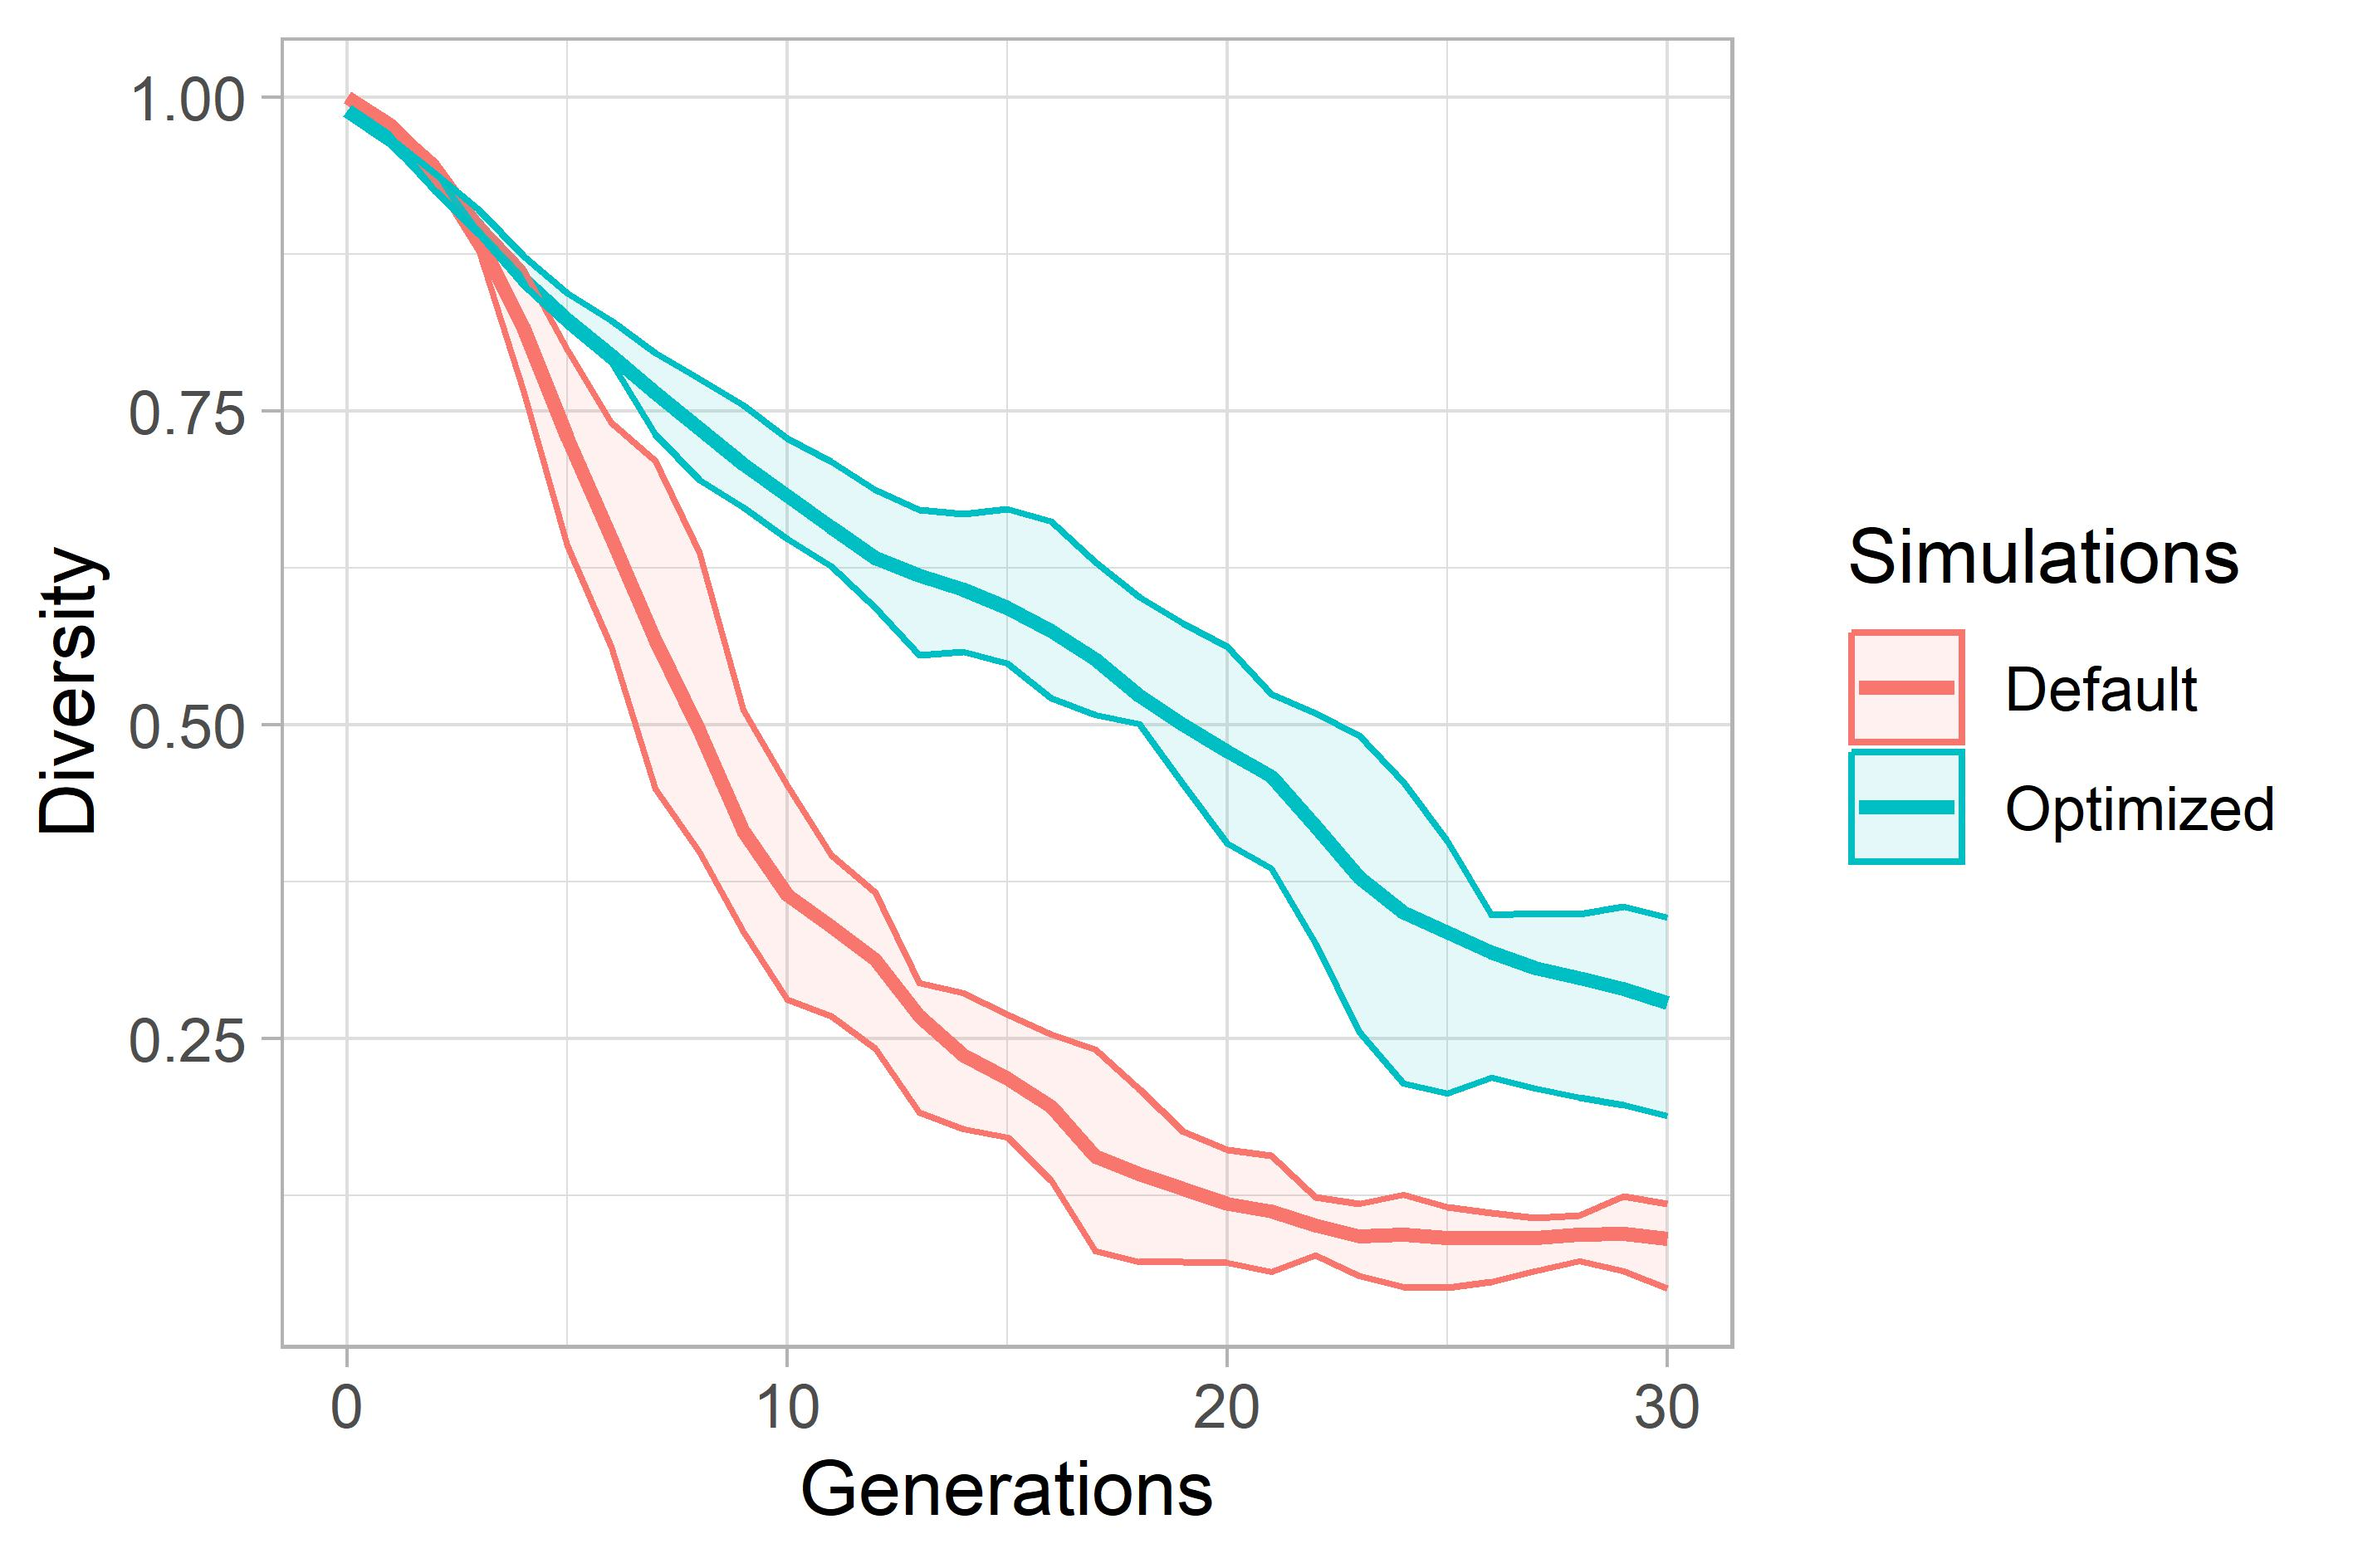
\includegraphics[width=1\linewidth]{simulations/evaluation/plots/sim_4_ga_diversity} 
	\end{minipage} 
	\caption{Start Scenario 4: Comparison of GAs}
\end{figure}

Already at generation 5, the average rate of improved fitness of the Default GA drops compared to the Optimized GA. This is accompanied by an early sharp decline in the diversity. The optimized GA again shows be able to hold the diversity much longer at a high level, its rate of diversity drop is linear.
The results underline the statement made in Section \ref{sect:evaluation:scenario_3}, which claims, that the Optimized GA excels at scenarios with lots of NPCs, where a vast search space is given.




\chapter{Conclusion}
\section{Test}
Altough lots of shortcommings
Results look very vielversprechend. This thesis hopes to have emphasised that this approach has lots of advanatages

\backmatter
\appendix                       %% closes main document, appendix follows until end; only available in book-classes
\addpart*{Appendix}             %% adding Appendix to tableofcontents
\chapter{Appendix A.}

\begin{figure}[ht] 
	\centering
	\begin{minipage}[b]{0.5\linewidth}
		\centering
		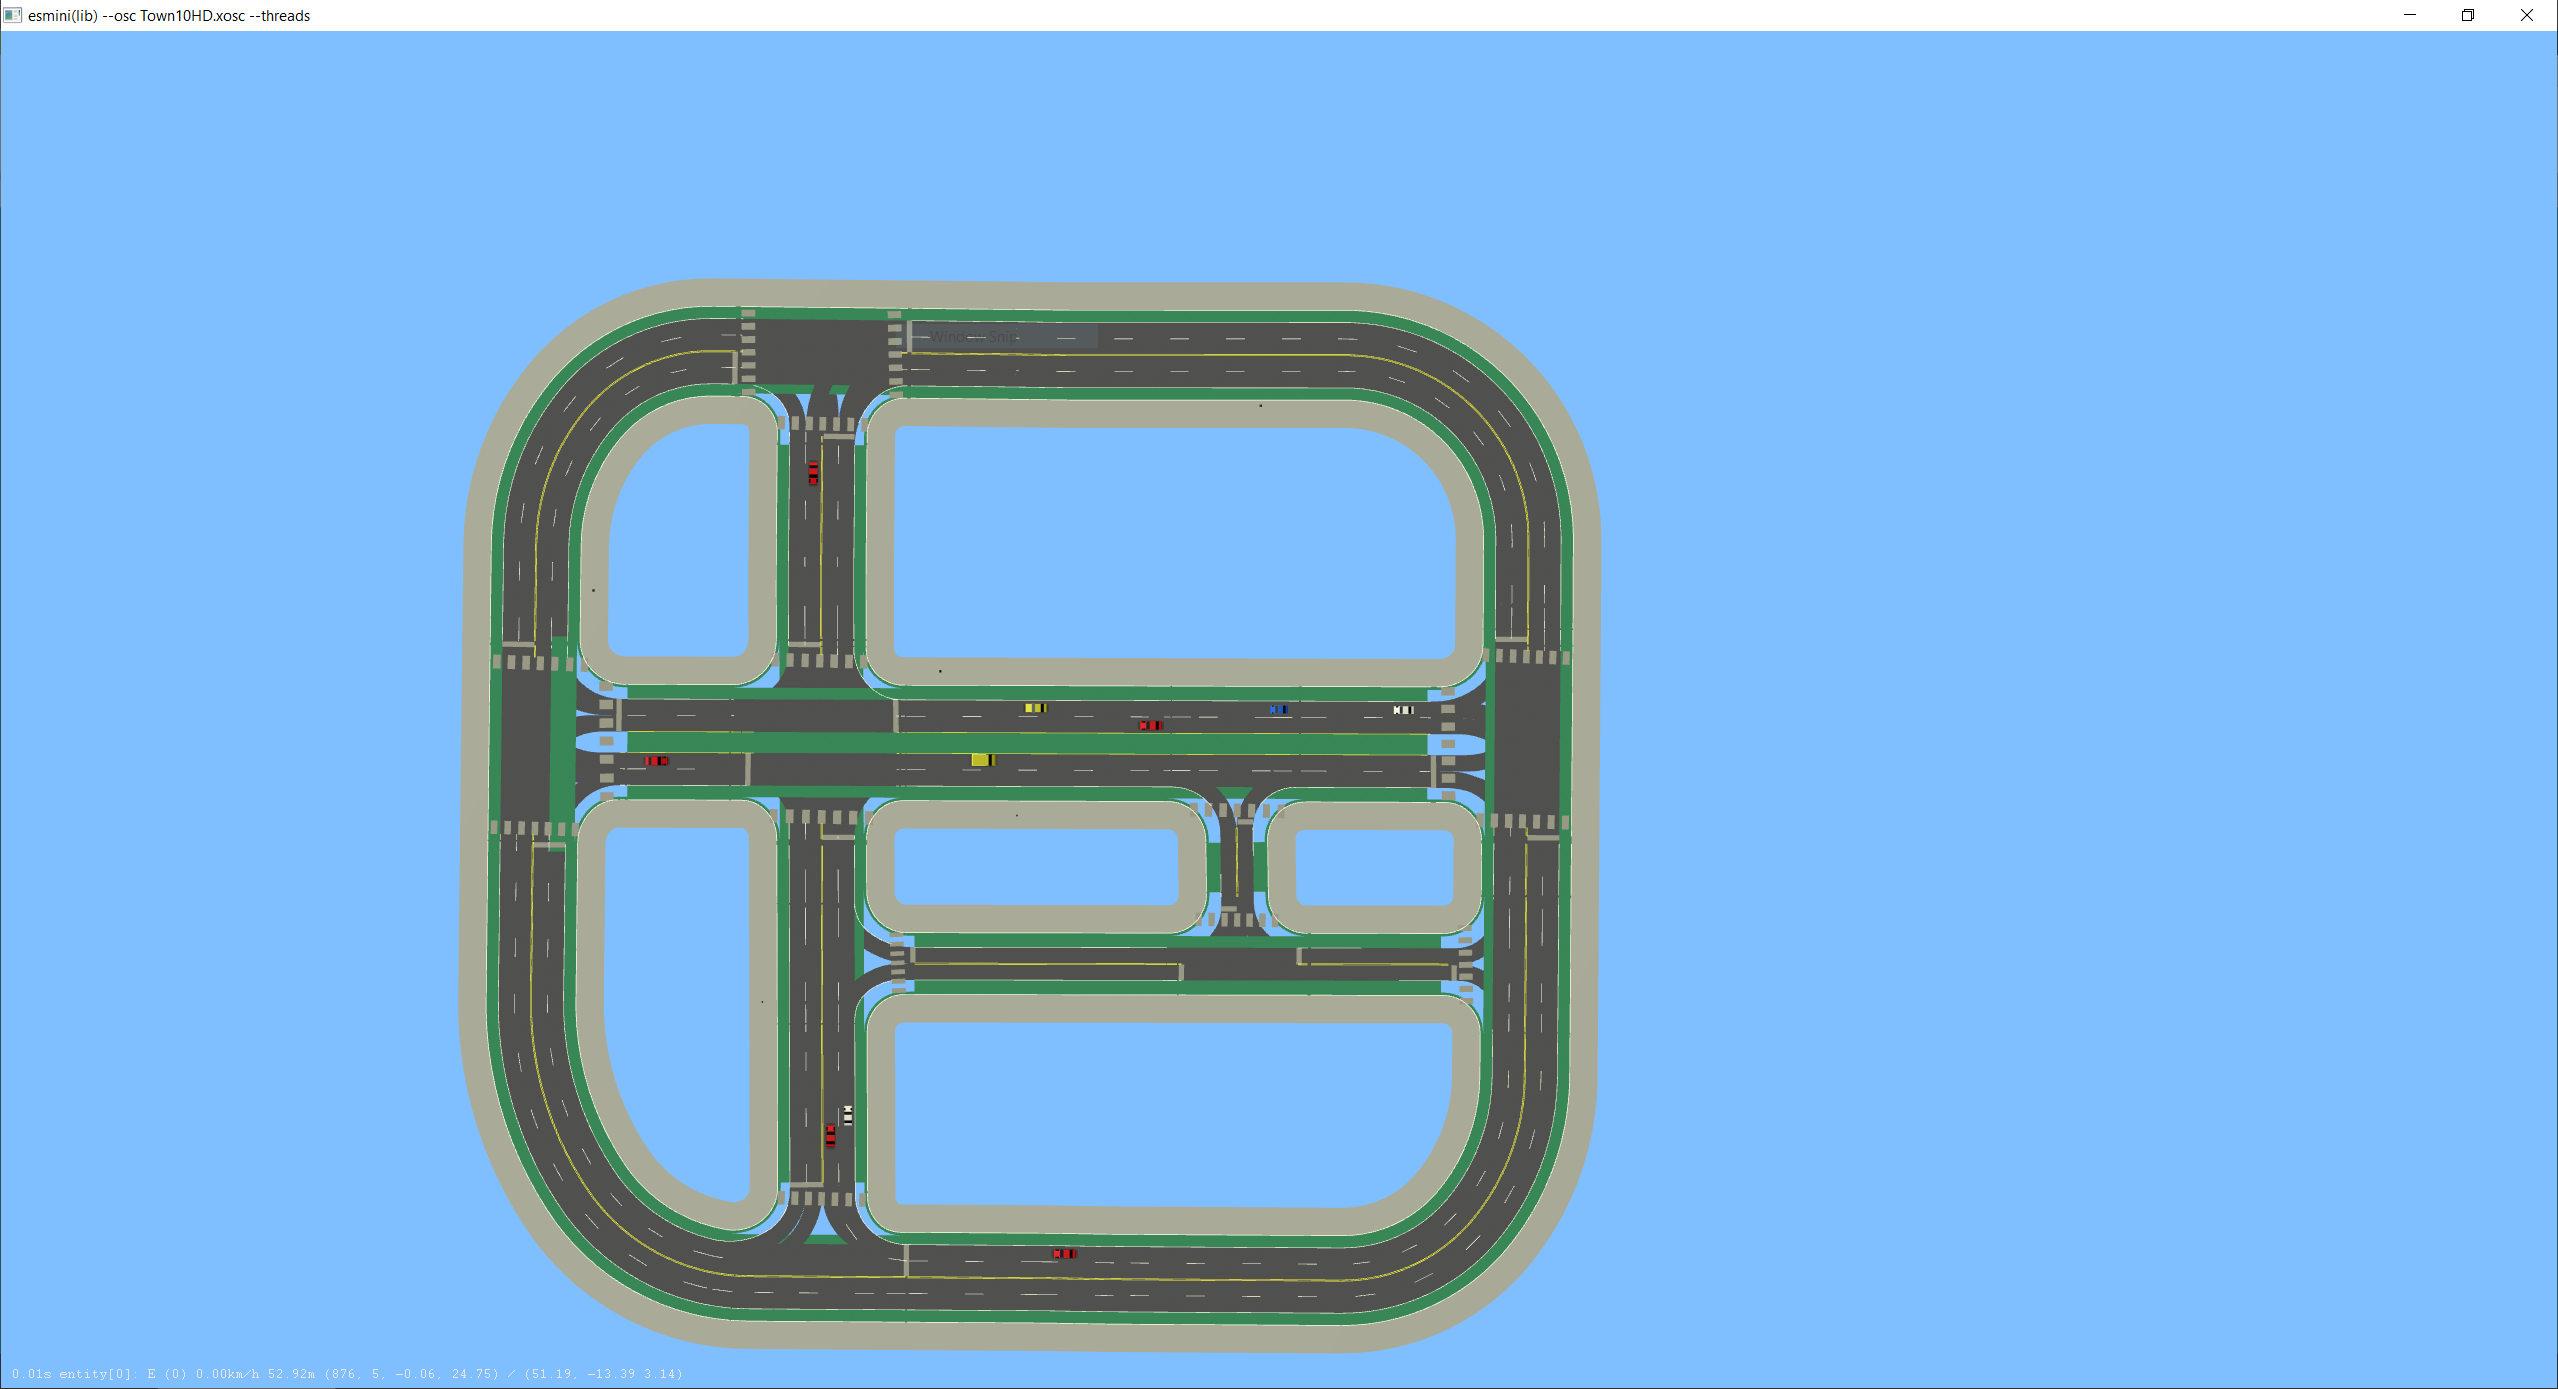
\includegraphics[width=1\linewidth]{figures/start_scenarios/scenario_1} 
		Start Scenario 1
	\end{minipage}%%
	\begin{minipage}[b]{0.5\linewidth}
		\centering
		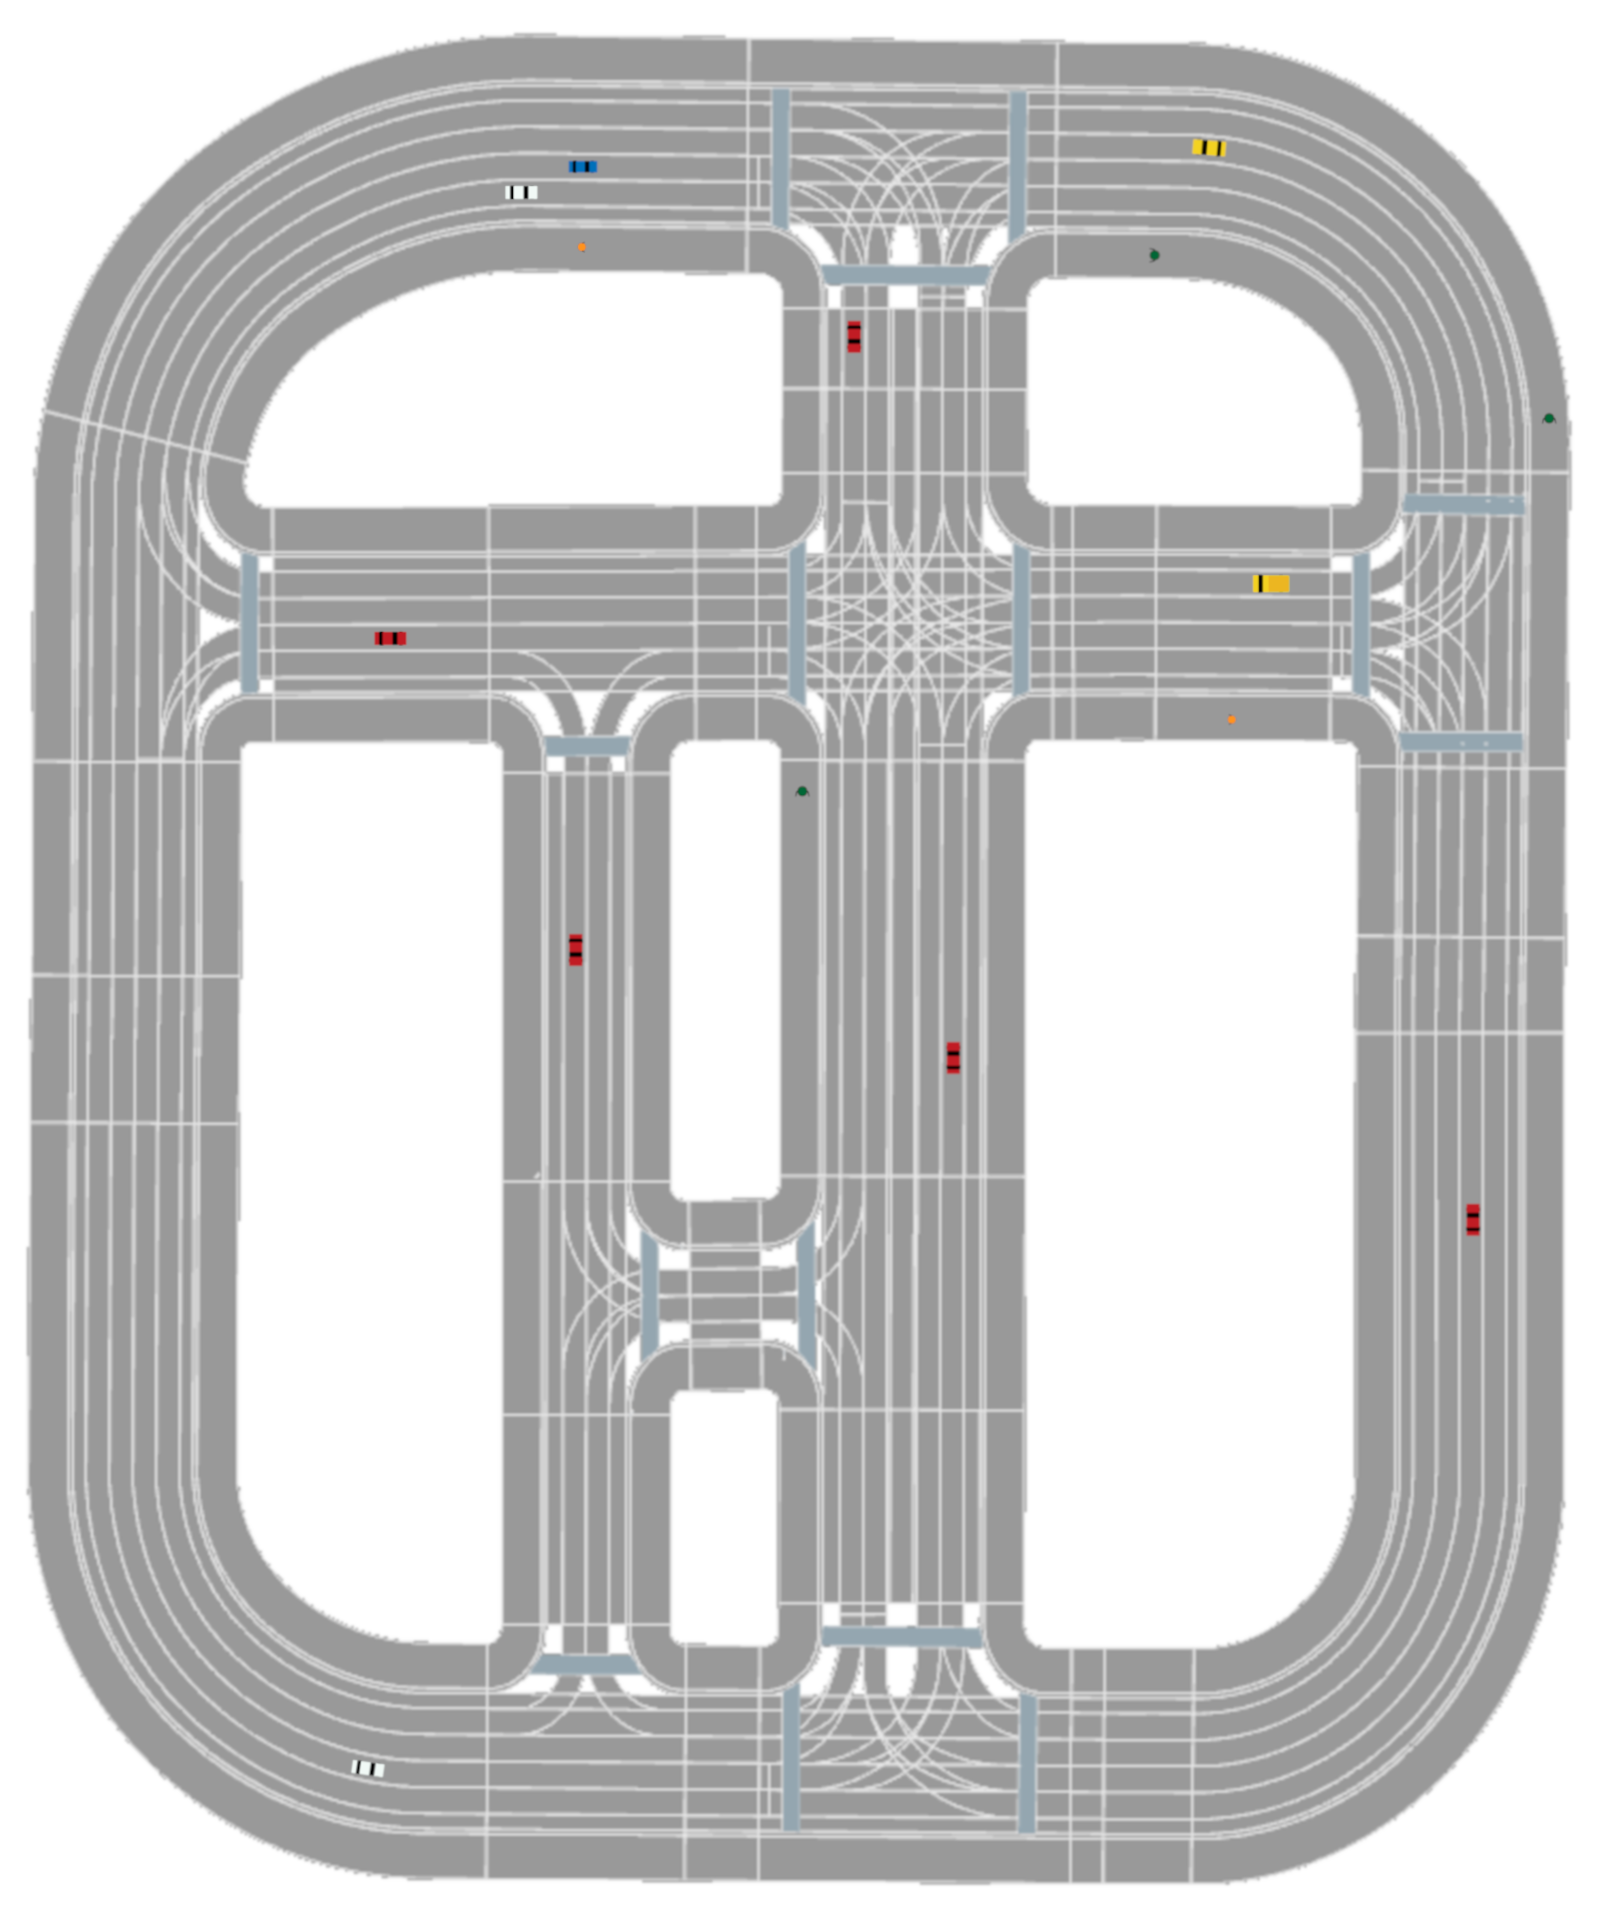
\includegraphics[width=1\linewidth]{figures/start_scenarios/scenario_2} 
		Start Scenario 2
	\end{minipage} 
	\caption{Visualization of Positions in Start Scenarios 1 and 2: Positions of all vehicles and pedestrians are depicted with the EGO vehicle drawn in blue.}
	\label{fig:appendix:start_scenarios_1_2} 
\end{figure}

\begin{figure}[ht] 
	\centering
	\begin{minipage}[b]{0.5\linewidth}
		\centering
		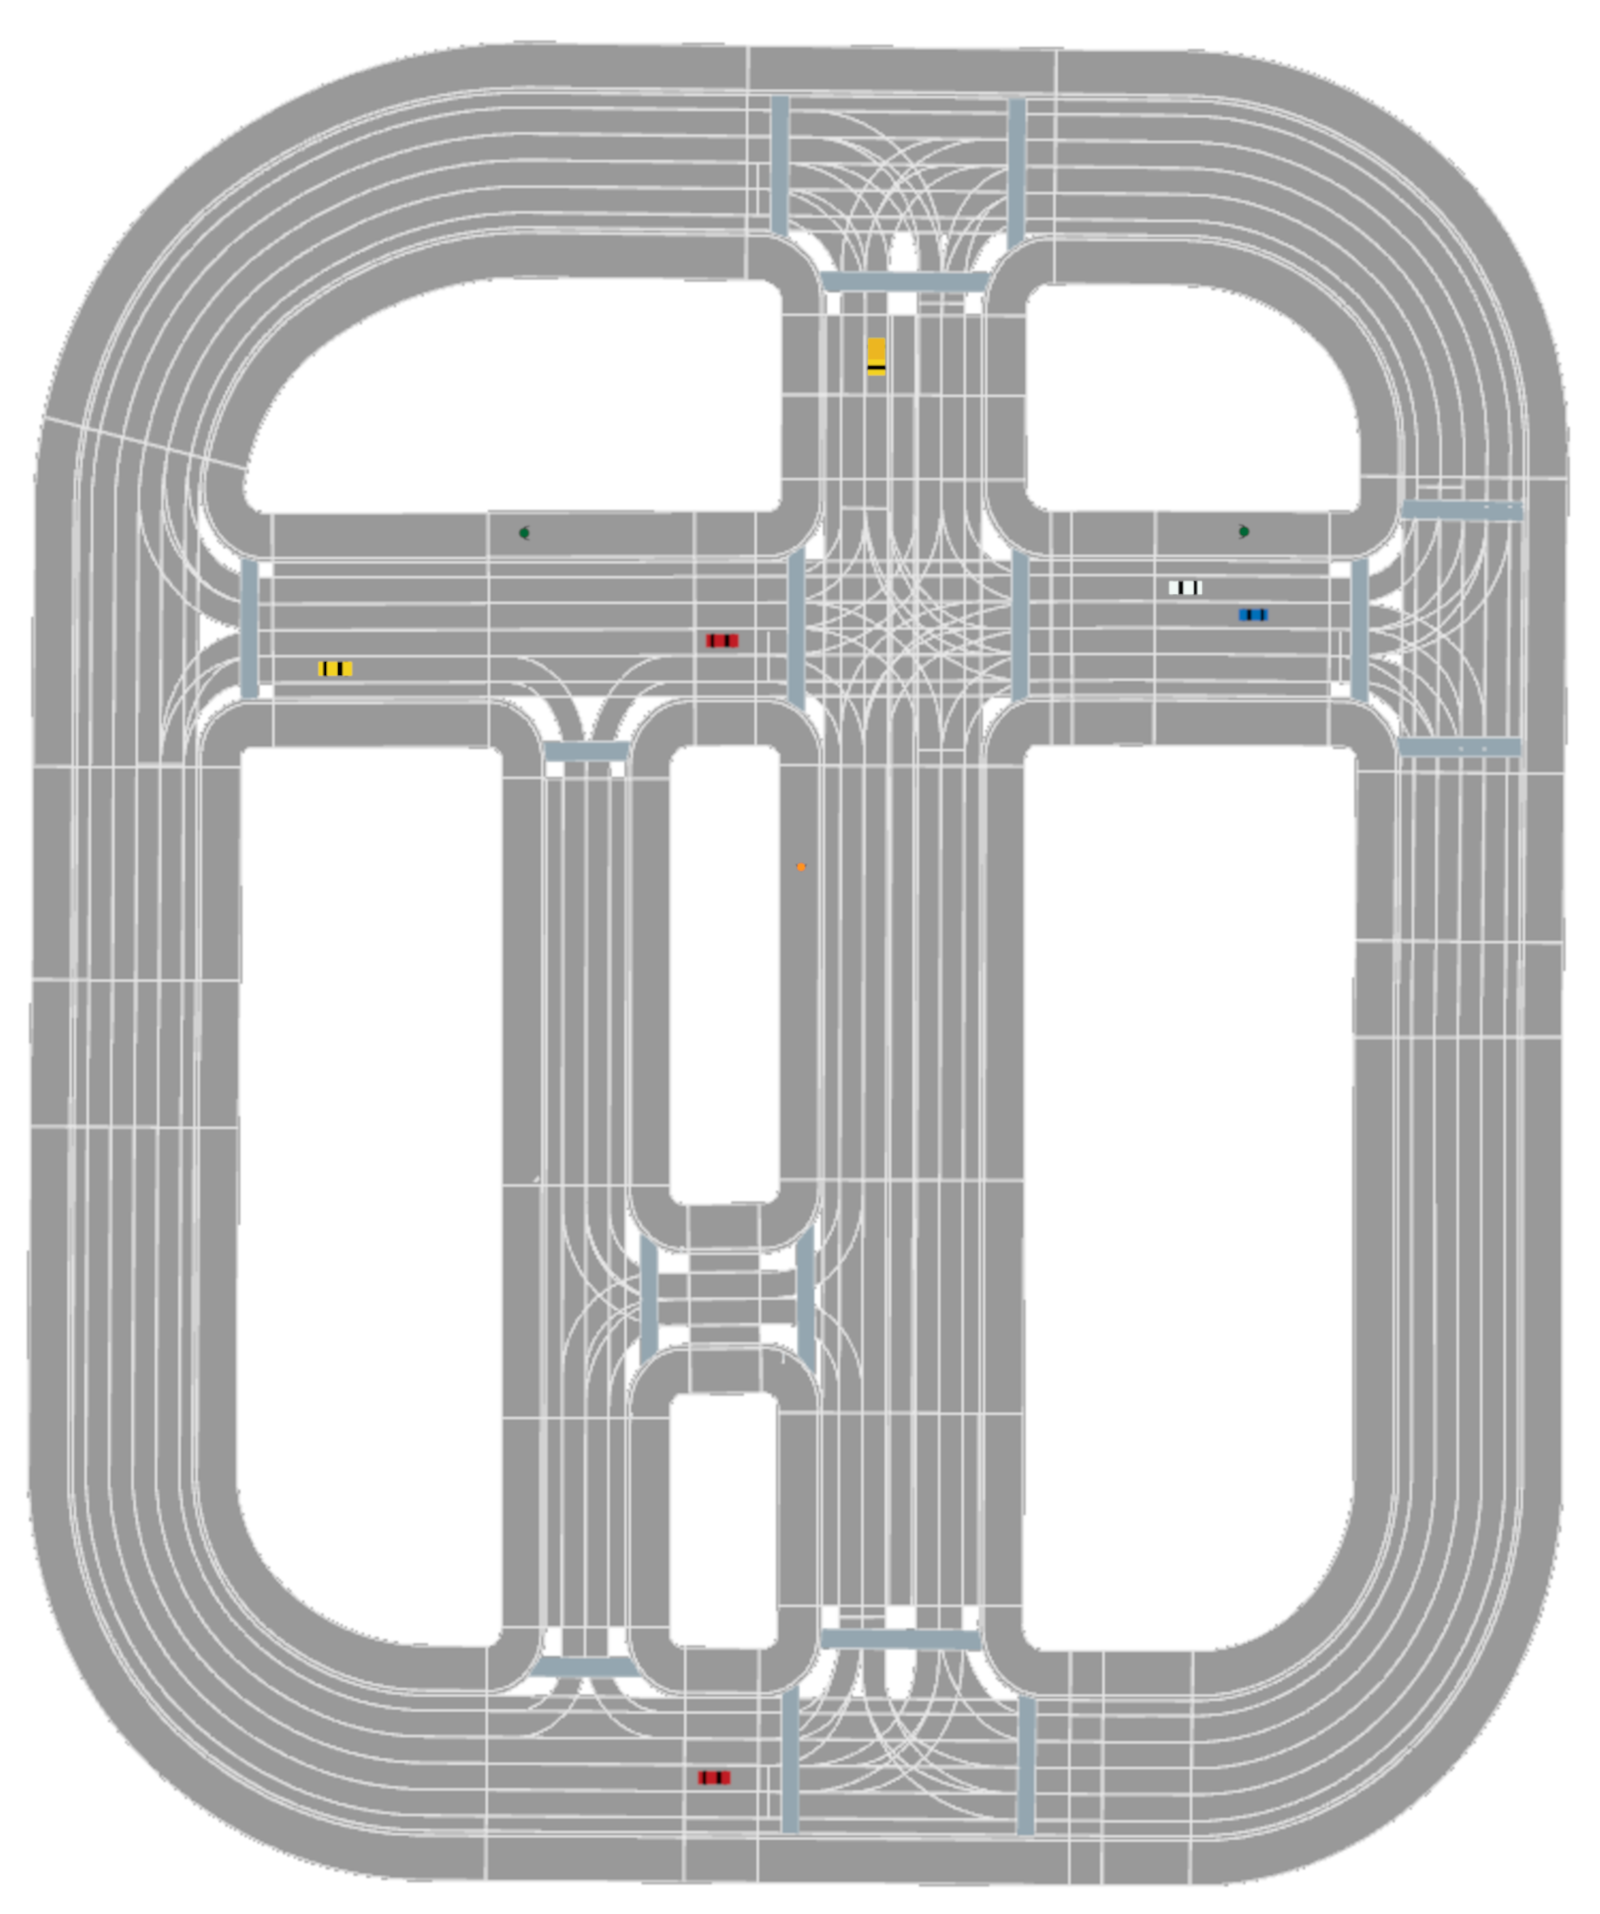
\includegraphics[width=1\linewidth]{figures/start_scenarios/scenario_3} 
		Start Scenario 3
	\end{minipage}%% 
	\begin{minipage}[b]{0.5\linewidth}
		\centering
		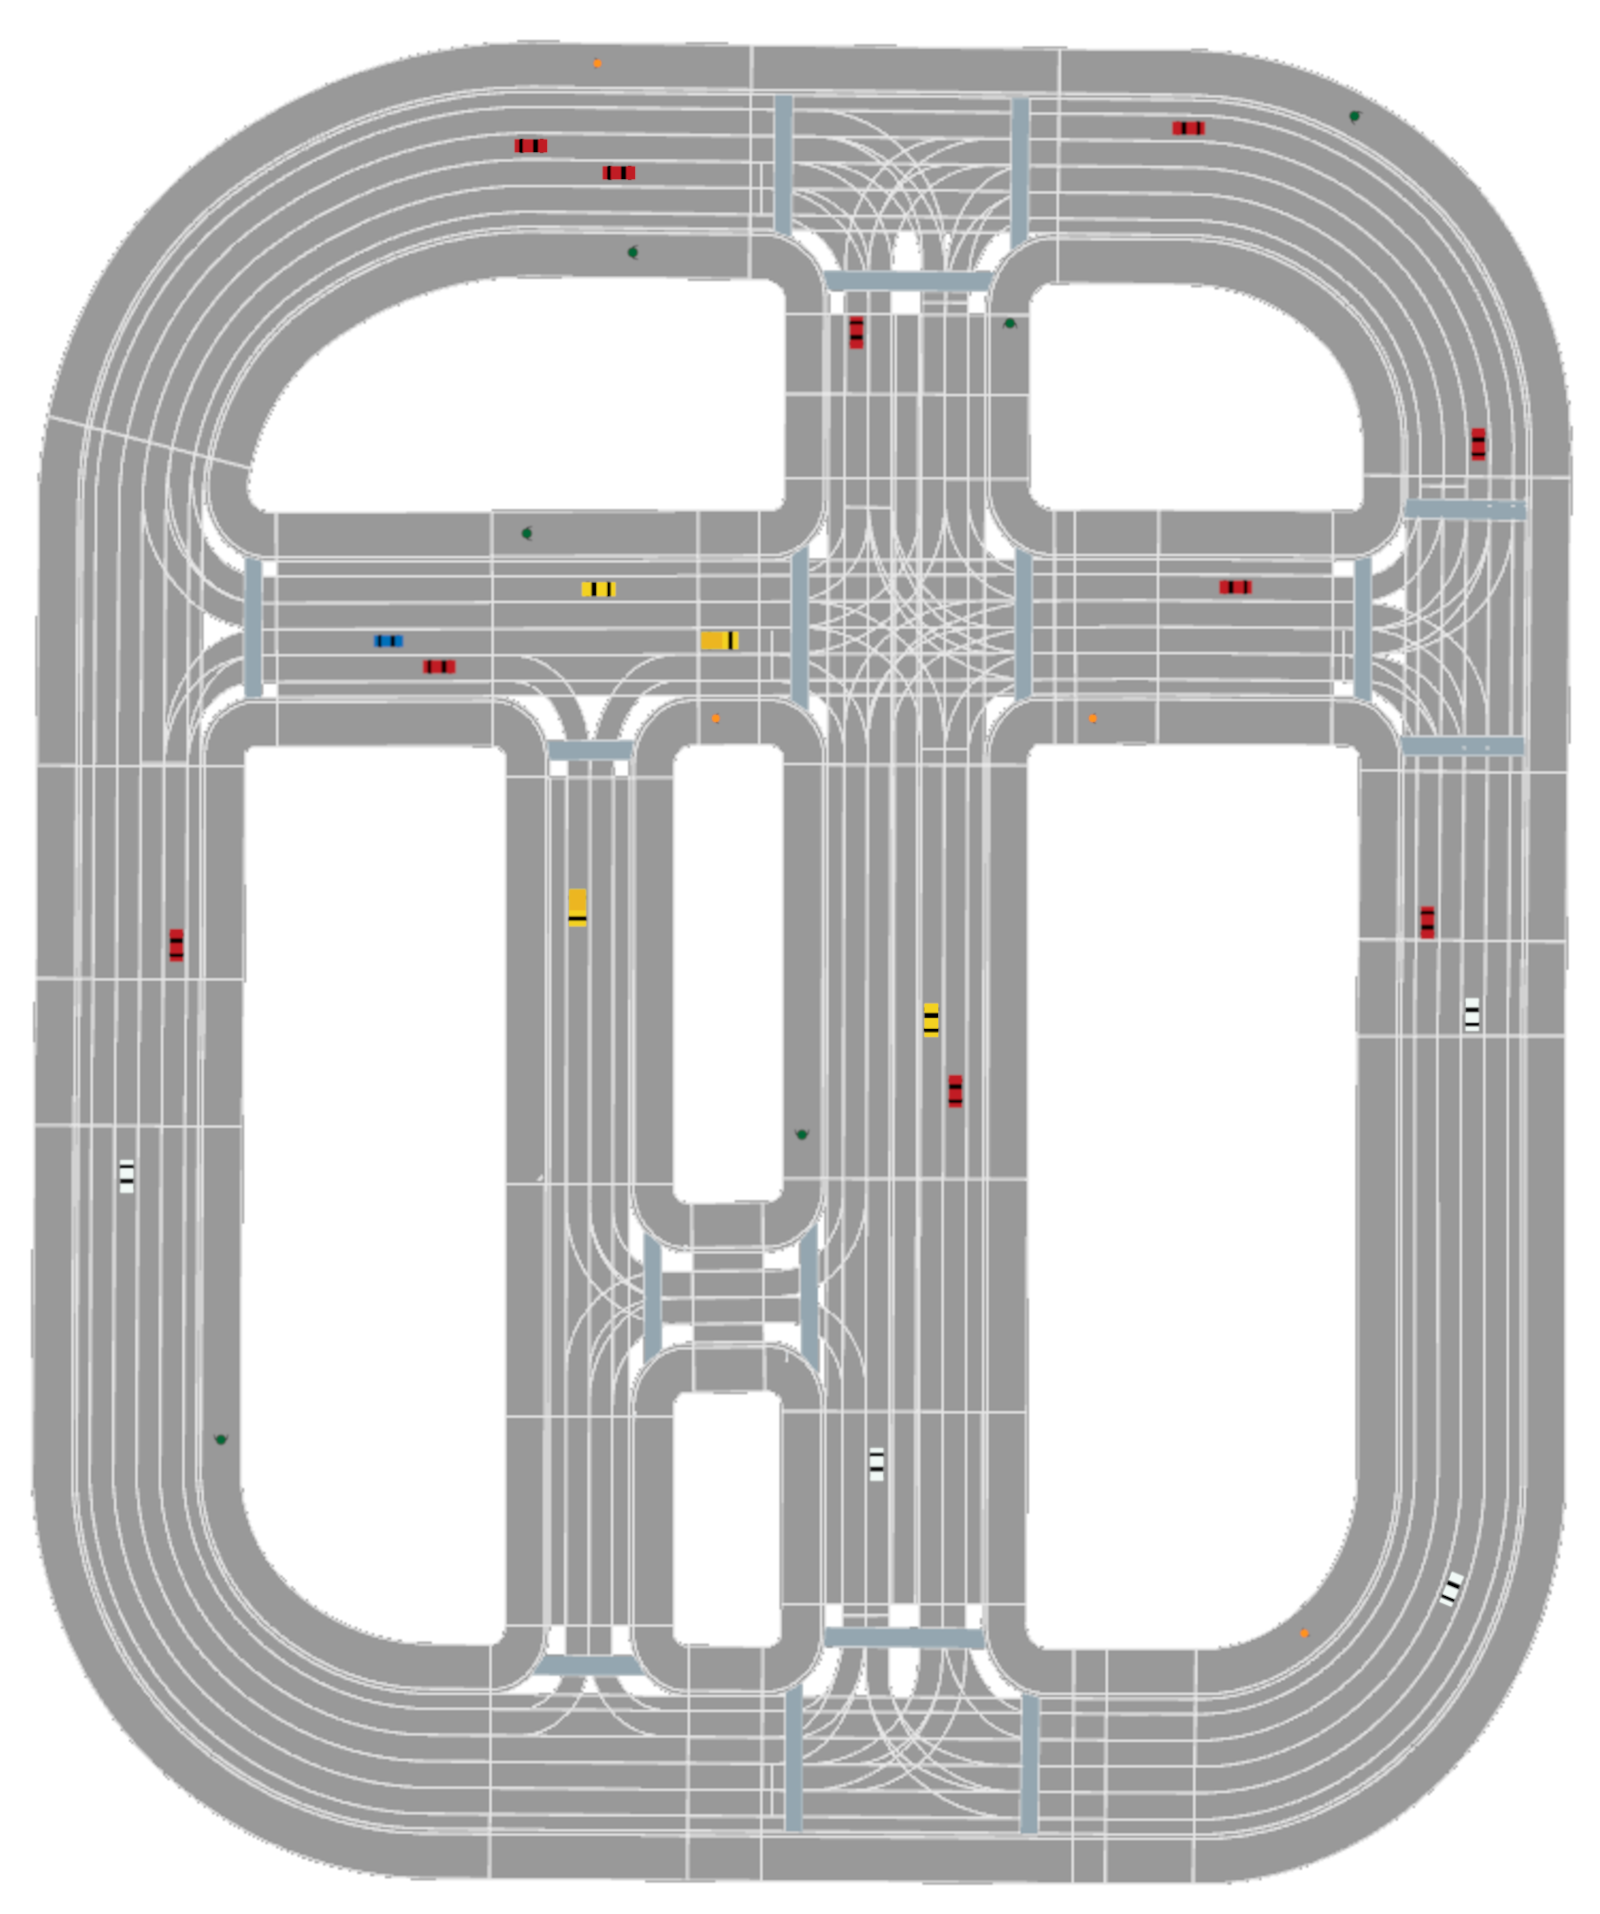
\includegraphics[width=1\linewidth]{figures/start_scenarios/scenario_4} 
		Start Scenario 4
	\end{minipage} 
	\caption{Visualization of Positions in Start Scenarios 3 and 4: Positions of all vehicles and pedestrians are depicted with the EGO vehicle drawn in blue.}
	\label{fig:appendix:start_scenarios_3_4} 
\end{figure}


\chapter{Appendix B.}

\begin{table}[ht]
	\centering
	\begin{tabular}{ rrrrrrrrr }
		\hline
		NO.& rep1 & rep2 & rep3 & rep4 & rep5 & rep6 & rep7 & rep8\\
  		\hline
		1 & 3.76 & 3.90 & 4.75 & 4.23 & 4.32 & 5.75 & 3.94 & 3.95 \\ 
		2 & 8.06 & 5.20 & 4.75 & 5.04 & 4.63 & 5.79 & 4.32 & 6.00 \\ 
		3 & 8.62 & 7.89 & 8.76 & 6.44 & 8.77 & 6.68 & 5.96 & 7.22 \\ 
		4 & 7.65 & 6.95 & 6.49 & 5.35 & 6.24 & 7.97 & 6.52 & 6.42 \\ 
		5 & 4.26 & 5.45 & 4.55 & 4.20 & 3.80 & 5.29 & 6.05 & 7.02 \\ 
		6 & 5.26 & 5.21 & 5.71 & 5.59 & 5.48 & 5.64 & 3.61 & 5.47 \\ 
		7 & 3.92 & 4.01 & 4.51 & 4.80 & 4.08 & 4.43 & 4.10 & 6.05 \\ 
		8 & 6.60 & 5.69 & 5.79 & 5.79 & 5.43 & 5.03 & 6.11 & 6.05 \\ 
		9 & 4.93 & 5.05 & 5.17 & 4.91 & 6.53 & 5.04 & 7.66 & 5.73 \\ 
		10 & 5.84 & 6.72 & 4.87 & 7.13 & 6.82 & 5.74 & 4.66 & 6.78 \\ 
		11 & 4.93 & 6.21 & 4.10 & 4.67 & 5.94 & 5.19 & 3.91 & 3.96 \\ 
		12 & 5.54 & 4.84 & 7.10 & 5.83 & 5.96 & 5.17 & 6.02 & 8.94 \\ 
		13 & 11.22 & 7.88 & 5.94 & 7.00 & 5.88 & 7.05 & 6.40 & 6.66 \\ 
		14 & 6.05 & 7.40 & 7.50 & 6.51 & 9.58 & 5.03 & 5.35 & 5.09 \\ 
		15 & 6.58 & 4.35 & 4.50 & 7.21 & 6.38 & 5.77 & 5.45 & 6.08 \\ 
		16 & 4.35 & 6.66 & 8.57 & 4.44 & 4.49 & 4.89 & 6.72 & 5.37 \\ 
		\hline
	\end{tabular}
	\caption{Table of Taguchi Experiment Results: A row corresponds to an experiment, each repeated eight times. The cumulated emergency break duration (in seconds) is shown.}
	\label{tab:appendix:hyperparameter_tuning_final_taguchi}
\end{table}

\begin{sidewaystable}
	\centering
	\begin{tabular}{ rrrrrrrrrrr }
		\hline
		scenario & rep1 & rep2 & rep3 & rep4 & rep5 & rep6 & rep7 & rep8 & rep9 & rep10\\
		\hline
		1 & 7.28 & 7.31 & 9.09 & 9.38 & 8.16 & 8.05 & 7.69 & 10.20 & 9.22 & 8.83 \\ 
		2 & 7.76 & 9.42 & 8.28 & 9.51 & 9.96 & 10.27 & 10.38 & 8.87 & 9.82 & 8.12 \\ 
		3 & 7.67 & 7.34 & 6.86 & 4.86 & 5.00 & 7.14 & 8.33 & 5.51 & 6.18 & 7.66 \\ 
		4 & 10.19 & 11.57 & 10.67 & 10.71 & 9.07 & 11.25 & 10.19 & 10.09 & 12.29 & 9.97 \\ 
		\hline
	\end{tabular}
	\caption{Optimized Genetic Algorithm Evaluation: The results of the optimized genetic algorithm over ten repetitions across four different start scenarios. The cumulated emergency break duration (in seconds) is shown.}
	\label{tab:appendix:evaluation_optimized}
	
	\vspace{2em}
	\begin{tabular}{ rrrrrrrrrrr }
		\hline
		scenario & rep1 & rep2 & rep3 & rep4 & rep5 & rep6 & rep7 & rep8 & rep9 & rep10\\
		\hline
		1 & 6.66 & 6.10 & 6.32 & 7.32 & 7.37 & 9.23 & 6.44 & 8.57 & 6.14 & 6.70 \\
		2 & 7.09 & 6.78 & 7.00 & 7.10 & 6.01 & 8.04 & 6.75 & 8.59 & 9.13 & 8.12 \\ 
		3 & 8.31 & 6.14 & 6.94 & 8.99 & 5.27 & 4.94 & 6.56 & 6.03 & 6.61 & 5.11 \\ 
		4 & 8.78 & 9.44 & 8.22 & 7.47 & 7.99 & 9.58 & 9.45 & 8.59 & 6.90 & 8.17 \\ 
		\hline
	\end{tabular}
	\caption{Default Genetic Algorithm Evaluation: The results of the default genetic algorithm over ten repetitions across four different start scenarios. The cumulated emergency break duration (in seconds) is shown.}
	\label{tab:appendix:evaluation_default}
	
	\vspace{2em}
	\begin{tabular}{ rrrrrrrrrrr }
		\hline
		scenario & rep1 & rep2 & rep3 & rep4 & rep5 & rep6 & rep7 & rep8 & rep9 & rep10\\
		\hline
		1 & 3.92 & 4.41 & 4.19 & 4.33 & 4.38 & 4.88 & 8.27 & 4.76 & 5.65 & 4.64 \\ 
		2 & 5.16 & 4.91 & 4.82 & 4.89 & 4.91 & 5.47 & 4.97 & 6.21 & 4.93 & 4.99 \\ 
		3 & 4.53 & 4.63 & 4.35 & 4.62 & 4.13 & 4.14 & 4.91 & 5.98 & 4.56 & 4.34 \\ 
		4 & 7.01 & 6.01 & 6.63 & 7.31 & 6.85 & 6.66 & 7.35 & 6.78 & 7.38 & 6.57 \\
		\hline
	\end{tabular}
	\caption{Random Search Evaluation: The results of the random search over ten repetitions across four different start scenarios. The cumulated emergency break duration (in seconds) is shown.}
	\label{tab:appendix:evaluation_random}
\end{sidewaystable}






\printbibliography              %% remove, if using BibTeX instead of biblatex
% \include{further_ressources}  %% this is a suggestion: you have to create this file on demand






%%%% end{document}
\end{document}
%% vim:foldmethod=expr
%% vim:fde=getline(v\:lnum)=~'^%%%%\ .\\+'?'>1'\:'='
%%% Local Variables:
%%% mode: latex
%%% mode: auto-fill
%%% mode: flyspell
%%% eval: (ispell-change-dictionary "en_US")
%%% TeX-master: "main"
%%% End:
